\documentclass{article} %definicion del tipo de documento

%Paquetes
\usepackage[utf8]{inputenc} %encoding
\usepackage{amsmath} %funciones matematicas avanzadas
\usepackage{amsfonts} %letras matematicas avanzadas
\usepackage{listings} %listas
\usepackage[a4paper, total={6in, 8in}]{geometry} %dimensiones del documento
\usepackage{graphicx} %importar imagenes
\usepackage{enumerate} %listas y enumerables
\usepackage{float} %posicion de objetos
\usepackage{pdfpages} %paginas de otros pdfs

%Configuraciones
\graphicspath{ {./images/} } %ruta de las imagenes
\setlength{\parindent}{0px} %0px de sangria en parrafos nuevos
\setlength{\parskip}{1em} %1em de espacio entre parrafos
\setlength{\jot}{12px} %12px de espacio vertical entre ecuaciones

\title{Tarea 2 - Cómputo Numérico}
\author{Daniel Uriel Orozco Lomeli}

\begin{document}
\maketitle

\section*{Ejercicio 1}
\textbf{1.} Considere el metodo de la secante para encontrar la raiz $x=\alpha$ de la funcion $f(x)$, en donde el proceso iterativo esta dado por,

\begin{equation}
\label{seceq}
    x_{i+1} = x_i - \frac{x_i - x_{i-1}}{f(x_i)-f(x_{i-1})}f(x_i)
\end{equation}

si $\epsilon_i=x_i-\alpha$ es el error asociado al proceso iterativo en el paso iésimo, demostrar que 

\begin{equation*}
    |\epsilon_{i+1}| = C|\epsilon_i|^\phi
\end{equation*}

en donde $C$ es una constante y $\phi = \frac{1 + \sqrt{5}}{2}$ es el cociente dorado.

\textbf{Demostración:}

Si $\epsilon_i=x_i-\alpha$ entonces sabemos que:

\begin{gather*}
    \epsilon_{i+1}=x_{i+1}-\alpha\\
    \epsilon_{i}=x_i-\alpha\\
    \epsilon_{i-1}=x_{i-1}-\alpha
\end{gather*}

por lo que, al despejar las $x_i$ obtenemos:

\begin{gather*}
    x_{i+1}=\epsilon_{i+1}+\alpha\\
    x_i=\epsilon_{i}+\alpha\\
    x_{i-1}=\epsilon_{i-1}+\alpha
\end{gather*}

al sustituir lo anterior en la ecuación \ref{seceq} obtenemos:

\begin{equation}
    \epsilon_{i+1} = \frac{\epsilon_{i-1}f(x_i) - \epsilon_{i}f(x_i)}{f(x_i)-f(x_{i-1})}
\end{equation}

Por el teorema del valor medio sabemos que existe un valor $a_i$ en el intervalo $[x_i,\alpha]$ tal que:

\begin{equation}
    f'(a_i) = \frac{f(x_i)-f(\alpha)}{x_i-\alpha}
\end{equation}

donde $\alpha$ al ser una raíz sabemos que $f(\alpha)=0$ y donde $x_i-\alpha=\epsilon_i$, por lo que al simplificar la ecuación anterior y despejar $f(x_i)$ obtenemos:

\begin{equation}
    f'(a_i) = \frac{f(x_i)}{\epsilon_i}, f(x_i) = \epsilon_i f'(a_i)
\end{equation}

y dado lo anterior, similarmente para el punto $x_{i-1}$ tenemos:

\begin{equation}
    f(x_{i-1}) = \epsilon_{i-1} f'(a_{i-1})
\end{equation}

Usando 2, 4 y 5 entonces:

\begin{equation}
    \epsilon_{i+1} = \epsilon_{i}\epsilon_{i-1}\frac{f'(a_{i}) - f'(a_{i-1})}{f(x_{i}) - f(x_{i-1})}
\end{equation}

donde 
\begin{equation*}
    \frac{f'(a_{i}) - f'(a_{i-1})}{f(x_{i}) - f(x_{i-1})}
\end{equation*}
no es mas que una constante $C$.

Al tener la ecuación 6 de la forma $\epsilon_{i+1} = C\epsilon_{i}\epsilon_{i-1}$, decimos que esta ecuación es de orden $p$ si:

\begin{gather*}
    \epsilon_i = C \epsilon_{i-i}^p\\
    \epsilon_{i+1} = C \epsilon_{i}^p\\
\end{gather*}

por lo que:

\begin{equation}
    \epsilon_{i+1}^p = C \epsilon_{i}^{(p+1)/{p}}
\end{equation}

de 7 entonces:

\begin{gather*}
    p = (p+1)/p\\
    p^2 = p + 1\\
    p^2 -p -1 = 0\\
    p = \frac{1 \pm \sqrt{1 + 4}}{2}\\
    \text{tomando la parte positiva, entonces}\\
    p = \frac{1 + \sqrt{5}}{2} = \phi
\end{gather*}

por lo que se demuestra que $|\epsilon_{i+1}| = C|\epsilon_i|^\phi$

\newpage
\section*{Ejercicio 2}
\textbf{2.} Considere la función $f(x) = \cos{(x)}-x$, y los tres puntos $\alpha_1 = -0.75$, $\alpha_2 = 1.25$ y $\alpha_3 = 3.15$

\textbf{a)} Grafique la función y cerciórese de que existe un cambio de signo entre $\alpha_1$ y $\alpha_2$.

\begin{center}
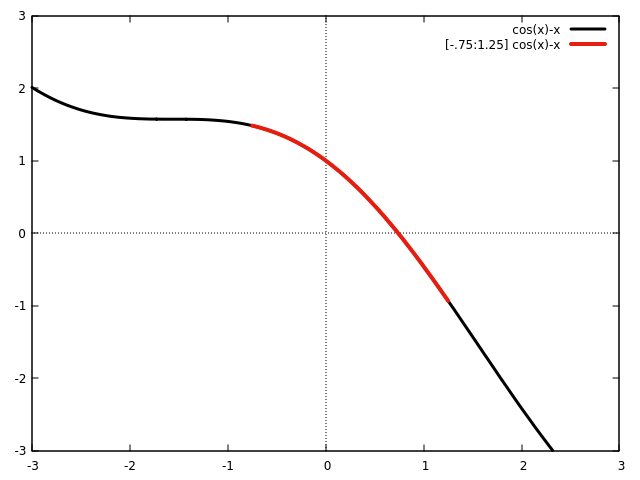
\includegraphics[scale=0.5]{images/grafica1.png}    
\end{center}

Se puede observar en el segmento rojo que cruza el 0 del eje y, por lo que si existe el cambio de signo.

\textbf{b)} Encuentre el cero de la función usando el método de bisección, correcto hasta 11
cifras significativas, tabulando los extremos del intervalo $[a, b]$ el punto medio $c$ y
$f(c)$ en cada paso del método para cuando los intervalos iniciales son: $[\alpha_1,\alpha_2]$ y $[\alpha_1,\alpha_3]$.

\begin{table}[H]
    \centering
    \begin{tabular}{|c|c|c|c|c|}
    \hline
it & $a$ & $b$ & $c$ & $f(c)$\\
\hline
0 & -0.75 & 1.25 & 0.25 & 0.71891242171\\
1 & 0.25 & 1.25 & 0.75 & -0.018311131126\\
2 & 0.25 & 0.75 & 0.5 & 0.37758256189\\
3 & 0.5 & 0.75 & 0.625 & 0.18596311951\\
4 & 0.625 & 0.75 & 0.6875 & 0.085334946152\\
5 & 0.6875 & 0.75 & 0.71875 & 0.033879372418\\
6 & 0.71875 & 0.75 & 0.734375 & 0.0078747254585\\
7 & 0.734375 & 0.75 & 0.7421875 & -0.0051957117438\\
8 & 0.734375 & 0.7421875 & 0.73828125 & 0.0013451497518\\
9 & 0.73828125 & 0.7421875 & 0.740234375 & -0.0019238727809\\
10 & 0.73828125 & 0.740234375 & 0.7392578125 & -0.00028900914679\\
11 & 0.73828125 & 0.7392578125 & 0.73876953125 & 0.00052815843366\\
12 & 0.73876953125 & 0.7392578125 & 0.73901367188 & 0.00011959667132\\
13 & 0.73901367188 & 0.7392578125 & 0.73913574219 & -8.4700731375e-05\\
14 & 0.73901367188 & 0.73913574219 & 0.73907470703 & 1.744934664e-05\\
$\vdots$ & $\vdots$ & $\vdots$ & $\vdots$ & $\vdots$\\
34 & 0.73908513319 & 0.7390851333 & 0.73908513325 & -5.1078363761e-11\\
35 & 0.73908513319 & 0.73908513325 & 0.73908513322 & -2.3698820684e-12\\
\hline
\end{tabular}
    \caption{Tabla método Bisección, intervalos $[\alpha_1,\alpha_2]$}
    \label{tab1}
\end{table}

\begin{table}[H]
    \centering
    \begin{tabular}{|c|c|c|c|c|}
    \hline
it & $a$ & $b$ & $c$ & $f(c)$\\
\hline
0 & -0.75 & 3.15 & 1.2 & -0.83764224552\\
1 & -0.75 & 1.2 & 0.225 & 0.74979410707\\
2 & 0.225 & 1.2 & 0.7125 & 0.044229923381\\
3 & 0.7125 & 1.2 & 0.95625 & -0.3796620853\\
4 & 0.7125 & 0.95625 & 0.834375 & -0.16273413814\\
5 & 0.7125 & 0.834375 & 0.7734375 & -0.057924032117\\
6 & 0.7125 & 0.7734375 & 0.74296875 & -0.0065052348029\\
7 & 0.7125 & 0.74296875 & 0.727734375 & 0.018948990059\\
8 & 0.727734375 & 0.74296875 & 0.7353515625 & 0.0062433917666\\
9 & 0.7353515625 & 0.74296875 & 0.73916015625 & -0.00012556153348\\
10 & 0.7353515625 & 0.73916015625 & 0.73725585938 & 0.0030602574375\\
11 & 0.73725585938 & 0.73916015625 & 0.73820800781 & 0.0014676832421\\
$\vdots$ & $\vdots$ & $\vdots$ & $\vdots$ & $\vdots$\\
35 & 0.73908513312 & 0.73908513323 & 0.73908513317 & 6.8257510755e-11\\
36 & 0.73908513317 & 0.73908513323 & 0.7390851332 & 2.0766610653e-11\\
37 & 0.7390851332 & 0.73908513323 & 0.73908513322 & -2.9787283751e-12\\
\hline
\end{tabular}
    \caption{Tabla método Bisección, intervalos $[\alpha_1,\alpha_3]$}
    \label{tab2}
\end{table}

\textbf{c)} Encuentre el cero de la función usando el método de punto fijo, correcto hasta 11 cifras significativas, tabulando $x_i$ y $f(x_i)$ en cada paso del método para cuando los puntos iniciales son: $x_1 =\alpha_1, x_1 =\alpha_2$ y $x_1 = \alpha_3$.

\begin{table}[H]
    \centering
    \begin{tabular}{|c|c|c|}
\hline
it & $x_i$ & $f(x_i)$\\
\hline
0 & -0.75 & 1.4816888689\\
1 & 0.73168886887 & 0.012358215915\\
2 & 0.74404708479 & -0.0083134666015\\
3 & 0.73573361819 & 0.0056049807007\\
4 & 0.74133859889 & -0.0037733025487\\
5 & 0.73756529634 & 0.002542763276\\
6 & 0.74010805962 & -0.0017123684894\\
7 & 0.73839569113 & 0.0011536828824\\
8 & 0.73954937401 & -0.00077703860825\\
9 & 0.7387723354 & 0.00052346602566\\
10 & 0.73929580143 & -0.00035259325102\\
11 & 0.73894320817 & 0.00023752001104\\
12 & 0.73918072819 & -0.00015999226962\\
13 & 0.73902073592 & 0.0001077745618\\
14 & 0.73912851048 & -7.2597404055e-05\\
15 & 0.73905591307 & 4.8902864452e-05\\
16 & 0.73910481594 & -3.2941385395e-05\\
17 & 0.73907187455 & 2.2189791661e-05\\
18 & 0.73909406434 & -1.4947275101e-05\\
$\vdots$ & $\vdots$ & $\vdots$\\
52 & 0.73908513323 & -2.1902590852e-11\\
53 & 0.73908513321 & 1.4753864797e-11\\
54 & 0.73908513322 & -9.9383834495e-12\\
\hline
\end{tabular}
    \caption{Tabla método Punto Fijo, con $x_1 = \alpha_1$}
    \label{tab3}
\end{table}


\begin{table}[H]
    \centering
    \begin{tabular}{|c|c|c|}
    \hline
it & $x_i$ & $f(x_i)$\\
\hline
0 & 1.25 & -0.9346776376\\
1 & 0.3153223624 & 0.63537409394\\
2 & 0.95069645633 & -0.36958001628\\
3 & 0.58111644006 & 0.25473385281\\
4 & 0.83585029287 & -0.1653031719\\
5 & 0.67054712097 & 0.11293467316\\
6 & 0.78348179413 & -0.075021234479\\
7 & 0.70846055965 & 0.050903876543\\
8 & 0.75936443619 & -0.034090718339\\
9 & 0.72527371785 & 0.023044164066\\
10 & 0.74831788192 & -0.015483451868\\
11 & 0.73283443005 & 0.010446786129\\
12 & 0.74328121618 & -0.0070291132001\\
13 & 0.73625210298 & 0.0047384249578\\
14 & 0.74099052794 & -0.0031902323872\\
15 & 0.73780029555 & 0.0021497094881\\
16 & 0.73995000504 & -0.001447736235\\
17 & 0.7385022688 & 0.00097536332215\\
18 & 0.73947763213 & -0.0006569478226\\
$\vdots$ & $\vdots$ & $\vdots$\\
63 & 0.73908513321 & 1.2473577726e-11\\
64 & 0.73908513322 & -8.4022788727e-12\\
\hline
\end{tabular}
    \caption{Tabla método Punto Fijo, con $x_1 = \alpha_2$}
    \label{tab4}
\end{table}

\begin{table}[H]
    \centering
    \begin{tabular}{|c|c|c|}
    \hline
it & $x_i$ & $f(x_i)$\\
\hline
0 & 3.15 & -4.1499646585\\
1 & -0.99996465847 & 1.5402967029\\
2 & 0.5403320444 & 0.3172058737\\
3 & 0.85753791811 & -0.20323655886\\
4 & 0.65430135924 & 0.13917195875\\
5 & 0.793473318 & -0.09209952576\\
6 & 0.70137379224 & 0.062582652321\\
7 & 0.76395644456 & -0.041851779297\\
8 & 0.72210466526 & 0.028311615784\\
9 & 0.75041628105 & -0.019011228859\\
10 & 0.73140505219 & 0.012831628274\\
11 & 0.74423668046 & -0.0086314831543\\
12 & 0.73560519731 & 0.0058195827248\\
13 & 0.74142478003 & -0.0039176824758\\
14 & 0.73750709756 & 0.0026400987854\\
15 & 0.74014719634 & -0.0017778983268\\
16 & 0.73836929802 & 0.0011978409988\\
17 & 0.73956713901 & -0.00080677654677\\
62 & 0.73908513321 & 1.5318524227e-11\\
63 & 0.73908513322 & -1.0318745858e-11\\
64 & 0.73908513321 & 6.9508843126e-12\\
\hline
\end{tabular}
    \caption{Tabla método Punto Fijo, con $x_1 = \alpha_3$}
    \label{tab5}
\end{table}
\begin{center}
\end{center}

\textbf{d)} Encuentre el cero de la función con el método de Newton, correcto hasta 13 cifras significativas, tabulando $x_i$ y $f(x_i)$ en cada paso del método para cuando los puntos iniciales son: $x_1 =\alpha_1, x_1 =\alpha_2$ y $x_1 = \alpha_3$. En cada caso, utilice la derivada:

\textbf{i)} Exacta, con $f'(x) = -\sin{(x)} -1$.

\textbf{ii)} Numérica, calculando la derivada hacia adelante con

\begin{equation*}
    f'(x) \approx \frac{f(x+\epsilon) - f(x)}{\epsilon}
\end{equation*}
con $\epsilon = 0.1$

\textbf{iii)} Numérica, calculando la derivada hacia atrás con

\begin{equation*}
    f'(x) \approx \frac{f(x) - f(x-\epsilon)}{\epsilon}
\end{equation*}
con $\epsilon = 0.1$

\textbf{iv)} Numérica, calculando la derivada con diferencias centrales con

\begin{equation*}
    f'(x) \approx \frac{f(x+\epsilon) - f(x-\epsilon)}{2\epsilon}
\end{equation*}
con $\epsilon = 0.1$

\textbf{v)} Repita los incisos \textbf{ii)},\textbf{iii)} y \textbf{iv)} pero con $\epsilon = 10^{-2}$ y $\epsilon = 10^{-4}$.

%%%%%%%%%%%%%%%%%%%%%%%%%%%%%%%%%%%%%%%%%%%%%%%%%%%%%%%%%%%%%%%%%%%%%%%%%%%%%%%%%%%%%%%
\begin{table}[H]
    \centering
    \begin{tabular}{|c|c|c|}
\hline
it & $x_i$ & $f(x_i)$\\
\hline
0 & -0.75 & 1.481688868874\\
1 & 3.904112004911 & -4.627210082022\\
2 & -11.05834832415 & 11.12108114118\\
3 & -5.492326215563 & 6.195561013016\\
4 & -1.871219105005 & 1.575295029316\\
5 & 33.30061678569 & -33.60938141361\\
6 & 16.0750934358 & -17.00845471628\\
7 & -10.45660443426 & 9.943352281013\\
8 & -5.105646687587 & 5.488846162885\\
9 & -2.252320137659 & 1.622342970371\\
10 & 5.010178240778 & -4.716770754768\\
11 & -102.158643887 & 102.101791912\\
12 & 63025.6761147 & -63025.09907882\\
13 & -280845.3779643 & 280846.2831857\\
14 & -83752.01839899 & 83751.06301727\\
15 & -19098.05385909 & 19097.10217375\\
16 & -4487.489534782 & 4487.761631095\\
17 & 114456.7014808 & -114457.2883032\\
18 & 51210.69540897 & -51211.61394414\\
19 & 14508.78741367 & -14508.17567477\\
20 & 6408.456989775 & -6407.532851938\\
21 & -3960.713005189 & 3960.042072903\\
22 & 11359.70237679 & -11358.74605818\\
$\vdots$ & $\vdots$ & $\vdots$\\
\hline
\end{tabular}
    \caption{Tabla método de Newton, con derivada exacta y con $x_1 = \alpha_1$}
    \label{tab6}
\end{table}

\begin{table}[H]
    \centering
    \begin{tabular}{|c|c|c|}
    \hline
it & $x_i$ & $f(x_i)$\\
\hline
0 & 1.25 & -0.9346776376047\\
1 & 0.7704284177913 & -0.05281605077596\\
2 & 0.7392950057892 & -0.000351261540583\\
3 & 0.7390851429387 & -1.627347179234e-08\\
4 & 0.7390851332152 & 0\\
\hline
\end{tabular}
    \caption{Tabla método de Newton, con derivada exacta y con $x_1 = \alpha_2$}
    \label{tab:newtonalhpa2extacta}
\end{table}

\begin{table}[H]
    \centering
    \begin{tabular}{|c|c|c|}
    \hline
it & $x_i$ & $f(x_i)$\\
\hline
0 & 3.15 & -4.149964658471\\
1 & -1.035150251908 & 1.545546982848\\
2 & 9.999667303452 & -10.83891978003\\
3 & -13.75644872841 & 14.12803608088\\
4 & 183.5569691319 & -183.3326921028\\
5 & 90.70797904375 & -91.62973643093\\
6 & 24.68123952276 & -23.7814466258\\
7 & -17.50817752624 & 17.73558827065\\
8 & -8.522668407894 & 7.90271229108\\
9 & 28.17209060215 & -29.16686830971\\
10 & 1.706444704833 & -1.841677466166\\
11 & 0.7813569779191 & -0.07139842879085\\
12 & 0.7394624773729 & -0.000631580334195\\
13 & 0.7390851646429 & -5.259782454026e-08\\
14 & 0.7390851332152 & -4.440892098501e-16\\
\hline
\end{tabular}
    \caption{Tabla método de Newton, con derivada exacta y con $x_1 = \alpha_3$}
    \label{tab:newtalp3ex}
\end{table}

%%%%%%%%%%%%%%%%%%%%%%%%%%%%%%%%%%%%%%%%%%%%%%%%%%%%%%%%%%%%%%%%%%%%%%%%%%%%%%%%%%%%%%%

\begin{table}[H]
\centering
\begin{tabular}{|c|c|c|}
\hline
it & $x_i$ & $f(x_i)$\\
\hline
0 & -0.75 & 1.481688868874\\
1 & 3.411454689905 & -4.37526237635\\
2 & -2.969312004647 & 1.984115646138\\
3 & -0.4243899932319 & 1.335680075135\\
4 & 1.680874899265 & -1.790731297349\\
5 & 0.7795621521449 & -0.0683407529021\\
6 & 0.7402254619365 & -0.001908948233189\\
7 & 0.7391092588921 & -4.037723825379e-05\\
8 & 0.7390856386037 & -8.458244158405e-07\\
9 & 0.7390851437999 & -1.771472413203e-08\\
10 & 0.7390851334368 & -3.710108886779e-10\\
11 & 0.7390851332198 & -7.770228904747e-12\\
12 & 0.7390851332153 & -1.626476731076e-13\\
13 & 0.7390851332152 & -3.441691376338e-15\\
\hline
\end{tabular}
\caption{Tabla método de Newton, con derivada numérica hacia adelante con $x_1 = \alpha_1$ y $\epsilon = 0.1$}
\end{table}

\begin{table}[H]
\centering
\begin{tabular}{|c|c|c|}
\hline
it & $x_i$ & $f(x_i)$\\
\hline
0 & -0.75 & 1.481688868874\\
1 & 4.486708710703 & -4.710478144037\\
2 & -118.9514449484 & 119.8607955452\\
3 & -31.45593421431 & 32.45513401389\\
4 & 4.203121316501 & -4.690659290209\\
5 & -26.51315346272 & 26.70238952451\\
6 & 2578.549628849 & -2579.315796663\\
7 & 1043.1023136 & -1042.106686454\\
8 & 44.45735657936 & -43.56809103852\\
9 & 13.60620608599 & -13.09984394566\\
10 & 6.469611153492 & -5.486938181433\\
11 & 1.639331969828 & -1.70781397194\\
12 & 0.7851737233301 & -0.07790825686091\\
13 & 0.7385342654868 & 0.000921826698313\\
14 & 0.7390980251308 & -2.157612644971e-05\\
15 & 0.7390848333736 & 5.018184585648e-07\\
16 & 0.7390851401899 & -1.167304919392e-08\\
17 & 0.7390851330529 & 2.71531797047e-10\\
18 & 0.7390851332189 & -6.316280831697e-12\\
19 & 0.7390851332151 & 1.468825061579e-13\\
20 & 0.7390851332152 & -3.441691376338e-15\\
\hline
\end{tabular}
\caption{Tabla método de Newton, con derivada numérica hacia atrás con $x_1 = \alpha_1$ y $\epsilon = 0.1$}
\end{table}

\begin{table}[H]
\centering
\begin{tabular}{|c|c|c|}
\hline
it & $x_i$ & $f(x_i)$\\
\hline
0 & -0.75 & 1.481688868874\\
1 & 3.887571213629 & -4.621995328042\\
2 & -10.44687422941 & 9.925295674093\\
3 & -5.087012304405 & 5.452934307645\\
4 & -2.260332601386 & 1.624153133966\\
5 & 4.809066747335 & -4.712539511272\\
6 & -739.9372393618 & 740.0292783589\\
7 & -368.8272021941 & 368.5222058383\\
8 & -179.915766145 & 179.252023561\\
9 & -77.29340770838 & 76.97467923321\\
10 & 1355.249642433 & -1355.590273094\\
11 & -20733.91187052 & 20734.73740757\\
12 & -7471.385547336 & 7472.164239894\\
13 & 12526.94165479 & -12527.10003644\\
14 & -865530.2418153 & 865529.3766906\\
15 & 868028.9328087 & -868028.107155\\
$\vdots$ & $\vdots$ & $\vdots$\\
44 & -2.560141836269 & 1.724475149017\\
45 & 1.257788327674 & -0.9498664571031\\
46 & 0.770634043085 & -0.05316489748262\\
47 & 0.7392762747323 & -0.000319910242898\\
48 & 0.7390850130272 & 2.011479619535e-07\\
49 & 0.7390851332958 & -1.349617084756e-10\\
50 & 0.7390851332151 & 9.059419880941e-14\\
\hline
\end{tabular}
\caption{Tabla método de Newton, con derivada numérica central con $x_1 = \alpha_1$ y $\epsilon = 0.1$}
\end{table}

%%%%%%%%%%%%%%%%%%%%%%%%%%%%%%%%%%%%%%%%%%%%%%%%%%%%%%%%%%%%%%%%%%%%%%%%%%%%%%%%%%%%%%%

\begin{table}[H]
\centering
\begin{tabular}{|c|c|c|}
\hline
it & $x_i$ & $f(x_i)$\\
\hline
0 & -0.75 & 1.481688868874\\
1 & 3.851075059578 & -4.609774219226\\
2 & -9.519261345977 & 8.523721581452\\
3 & -1.694765226469 & 1.571113614516\\
4 & 220.4463119306 & -219.5859546934\\
5 & 75.40789328121 & -74.40794003138\\
6 & 2.075664288928 & -2.559356168863\\
7 & 0.7090747454961 & 0.04988991792561\\
8 & 0.7392212455868 & -0.0002278061486305\\
9 & 0.7390854362109 & -5.070974210541e-07\\
10 & 0.7390851338807 & -1.113868886016e-09\\
11 & 0.7390851332166 & -2.446598479366e-12\\
12 & 0.7390851332152 & -5.440092820663e-15\\
\hline
\end{tabular}
\caption{Tabla método de Newton, con derivada numérica hacia adelante con $x_1 = \alpha_1$ y $\epsilon = 10^{-2}$}
\end{table}

\begin{table}
\centering
\begin{tabular}{|c|c|c|}
\hline
it & $x_i$ & $f(x_i)$\\
\hline
0 & -0.75 & 1.481688868874\\
1 & 3.958046003171 & -4.642856032952\\
2 & -12.94261091292 & 13.87266353194\\
3 & 9.150096208054 & -10.11260777602\\
4 & 1.22515704063 & -0.8863588160151\\
5 & 0.7680706413295 & -0.04881821417724\\
6 & 0.7392036140125 & -0.0001982960749334\\
7 & 0.7390848733763 & 4.348694726541e-07\\
8 & 0.7390851337919 & -9.652877386301e-10\\
9 & 0.7390851332139 & 2.142730437527e-12\\
10 & 0.7390851332152 & -4.884981308351e-15\\
\hline
\end{tabular}
\caption{Tabla método de Newton, con derivada numérica hacia atrás con $x_1 = \alpha_1$ y $\epsilon = 10^{-2}$}
\end{table}

\begin{table}
\centering
\begin{tabular}{|c|c|c|}
\hline
it & $x_i$ & $f(x_i)$\\
\hline
0 & -0.75 & 1.481688868874\\
1 & 3.903945930775 & -4.627158712855\\
2 & -11.05198357989 & 11.10836296117\\
3 & -5.493335107229 & 6.197286825938\\
4 & -1.86969085075 & 1.575226926051\\
5 & 33.64572280106 & -34.25804930566\\
6 & 14.51347332243 & -14.88096113635\\
7 & 6.803182044416 & -5.93536124354\\
8 & 2.837997954162 & -3.7922659669\\
9 & -0.08149347904222 & 1.078174722796\\
10 & 1.09222414733 & -0.6317119116314\\
11 & 0.757566907151 & -0.03105683371433\\
12 & 0.739158978098 & -0.0001235896992847\\
13 & 0.7390851339238 & -1.185909370705e-09\\
14 & 0.7390851332152 & 7.993605777301e-15\\
\hline
\end{tabular}
\caption{Tabla método de Newton, con derivada numérica central con $x_1 = \alpha_1$ y $\epsilon = 10^{-2}$}
\end{table}
%%%%%%%%%%%%%%%%%%%%%%%%%%%%%%%%%%%%%%%%%%%%%%%%%%%%%%%%%%%%%%%%%%%%%%%%%%%%%%%%%%%%%%%

\begin{table}
\centering
\begin{tabular}{|c|c|c|}
\hline
it & $x_i$ & $f(x_i)$\\
\hline
0 & -0.75 & 1.481688868874\\
1 & 3.903577223009 & -4.627044594827\\
2 & -11.04140368885 & 11.08721704898\\
3 & -5.494889639004 & 6.199944609512\\
4 & -1.867468344657 & 1.575129111409\\
5 & 34.20085775123 & -35.13792544626\\
6 & 8.155418036917 & -8.452310186383\\
7 & 3.831756090103 & -4.602898061382\\
8 & -8.837995100088 & 8.005268833262\\
9 & 9.100039320984 & -10.04777346964\\
10 & 1.482397899159 & -1.394114554923\\
11 & 0.7839786395834 & -0.07586881624594\\
12 & 0.7395104730202 & -0.0007119206609268\\
13 & 0.7390851825291 & -8.253234795585e-08\\
14 & 0.7390851332163 & -1.823208251039e-12\\
15 & 0.7390851332152 & 0\\
\hline
\end{tabular}
\caption{Tabla método de Newton, con derivada numérica hacia adelante con $x_1 = \alpha_1$ y $\epsilon = 10^{-4}$}
\end{table}

\begin{table}
\centering
\begin{tabular}{|c|c|c|}
\hline
it & $x_i$ & $f(x_i)$\\
\hline
0 & -0.75 & 1.481688868874\\
1 & 3.90464687648 & -4.627375390112\\
2 & -11.0753272129 & 11.15499561999\\
3 & -5.488939884478 & 6.189763116371\\
4 & -1.876167263419 & 1.575520292109\\
5 & 32.16739504507 & -31.43670795756\\
6 & 13.48482733025 & -12.87778005621\\
7 & 6.309118940922 & -5.309455198755\\
8 & 1.133609768334 & -0.7102174515726\\
9 & 0.7609731994119 & -0.03680798976261\\
10 & 0.7391880427727 & -0.0001722345868066\\
11 & 0.7390851332813 & -1.106427172104e-10\\
12 & 0.7390851332152 & 2.331468351713e-15\\
\hline
\end{tabular}
\caption{Tabla método de Newton, con derivada numérica hacia atrás con $x_1 = \alpha_1$ y $\epsilon = 10^{-4}$}
\end{table}

\begin{table}
\centering
\begin{tabular}{|c|c|c|}
\hline
it & $x_i$ & $f(x_i)$\\
\hline
0 & -0.75 & 1.481688868874\\
1 & 3.904111988285 & -4.62721007688\\
2 & -11.05834768688 & 11.12107986789\\
3 & -5.492326322269 & 6.195561195586\\
4 & -1.871218943667 & 1.57529502209\\
5 & 33.30065302844 & -33.60945212803\\
6 & 16.07499462156 & -17.0083913657\\
7 & -10.45278778456 & 9.936263784217\\
8 & -5.099983895122 & 5.477946727653\\
9 & -2.255510090066 & 1.623058771639\\
10 & 4.945286501259 & -4.714488719974\\
11 & -169.6766434648 & 170.6761740915\\
12 & 6.393506011222 & -5.399585170724\\
13 & 1.529440190601 & -1.488095842172\\
14 & 0.7850740363143 & -0.07773809981705\\
15 & 0.7395299960881 & -0.0007446009791902\\
16 & 0.7390851768925 & -7.309894500818e-08\\
17 & 0.7390851332152 & -5.551115123126e-16\\
\hline
\end{tabular}
\caption{Tabla método de Newton, con derivada numérica central con $x_1 = \alpha_1$ y $\epsilon = 10^{-4}$}
\end{table}

%%%%%%%%%%%%%%%%%%%%%%%%%%%%%%%%%%%%%%%%%%%%%%%%%%%%%%%%%%%%%%%%%%%%%%%%%%%%%%%%%%%%%%%

\begin{table}[H]
\centering
\begin{tabular}{|c|c|c|}
\hline
it & $x_i$ & $f(x_i)$\\
\hline
0 & 1.25 & -0.9346776376047\\
1 & 0.7738904707096 & -0.05869352107821\\
2 & 0.740031859657 & -0.001584783883836\\
3 & 0.7391051286728 & -3.346478611543e-05\\
4 & 0.7390855520677 & -7.009967817329e-07\\
5 & 0.7390851419875 & -1.468148114192e-08\\
6 & 0.7390851333989 & -3.074837051642e-10\\
7 & 0.739085133219 & -6.439848654338e-12\\
8 & 0.7390851332152 & -1.347810751895e-13\\
9 & 0.7390851332152 & -2.886579864025e-15\\
\hline
\end{tabular}
\caption{Tabla método de Newton, con derivada numérica hacia adelante con $x_1 = \alpha_2$ y $\epsilon = 0.1$}
\end{table}

\begin{table}[H]
\centering
\begin{tabular}{|c|c|c|}
\hline
it & $x_i$ & $f(x_i)$\\
\hline
0 & 1.25 & -0.9346776376047\\
1 & 0.7661249409486 & -0.04552210302764\\
2 & 0.7386389507405 & 0.0007466627787649\\
3 & 0.7390955631862 & -1.745576513446e-05\\
4 & 0.7390848906272 & 4.059981804083e-07\\
5 & 0.7390851388581 & -9.444119819513e-09\\
6 & 0.7390851330839 & 2.196836046409e-10\\
7 & 0.7390851332182 & -5.110134537745e-12\\
8 & 0.7390851332151 & 1.189048859374e-13\\
9 & 0.7390851332152 & -2.886579864025e-15\\
\hline
\end{tabular}
\caption{Tabla método de Newton, con derivada numérica hacia atrás con $x_1 = \alpha_2$ y $\epsilon = 0.1$}
\end{table}

\begin{table}[H]
\centering
\begin{tabular}{|c|c|c|}
\hline
it & $x_i$ & $f(x_i)$\\
\hline
0 & 1.25 & -0.9346776376047\\
1 & 0.7700391143815 & -0.05215567421902\\
2 & 0.739268870942 & -0.0003075181447841\\
3 & 0.7390850173828 & 1.938584230921e-07\\
4 & 0.7390851332929 & -1.300705099183e-10\\
5 & 0.7390851332151 & 8.726352973554e-14\\
\hline
\end{tabular}
\caption{Tabla método de Newton, con derivada numérica central con $x_1 = \alpha_2$ y $\epsilon = 0.1$}
\end{table}


%%%%%%%%%%%%%%%%%%%%%%%%%%%%%%%%%%%%%%%%%%%%%%%%%%%%%%%%%%%%%%%%%%%%%%%%%%%%%%%%%%%%%%%
\begin{table}[H]
\centering
\begin{tabular}{|c|c|c|}
\hline
it & $x_i$ & $f(x_i)$\\
\hline
0 & 1.25 & -0.9346776376047\\
1 & 0.7708121601317 & -0.05346710051403\\
2 & 0.7393663471048 & -0.0004706721698918\\
3 & 0.7390857680818 & -1.062520624373e-06\\
4 & 0.7390851346097 & -2.333964577161e-09\\
5 & 0.7390851332182 & -5.126454816207e-12\\
6 & 0.7390851332152 & -1.143529715364e-14\\
\hline
\end{tabular}
\caption{Tabla método de Newton, con derivada numérica hacia adelante con $x_1 = \alpha_2$ y $\epsilon = 10^{-2}$}
\end{table}

\begin{table}[H]
\centering
\begin{tabular}{|c|c|c|}
\hline
it & $x_i$ & $f(x_i)$\\
\hline
0 & 1.25 & -0.9346776376047\\
1 & 0.7700362641298 & -0.05215083972952\\
2 & 0.739224457561 & -0.0002331820741358\\
3 & 0.7390848283157 & 5.10283388655e-07\\
4 & 0.739085133892 & -1.13269038593e-09\\
5 & 0.7390851332137 & 2.514100039264e-12\\
6 & 0.7390851332152 & -5.662137425588e-15\\
\hline
\end{tabular}
\caption{Tabla método de Newton, con derivada numérica hacia atrás con $x_1 = \alpha_2$ y $\epsilon = 10^{-2}$}
\end{table}

\begin{table}[H]
\centering
\begin{tabular}{|c|c|c|}
\hline
it & $x_i$ & $f(x_i)$\\
\hline
0 & 1.25 & -0.9346776376047\\
1 & 0.7704245259574 & -0.05280944850791\\
2 & 0.7392947415435 & -0.000350819254853\\
3 & 0.739085141508 & -1.387905956829e-08\\
4 & 0.7390851332151 & 9.303668946359e-14\\
\hline
\end{tabular}
\caption{Tabla método de Newton, con derivada numérica central con $x_1 = \alpha_2$ y $\epsilon = 10^{-2}$}
\end{table}
%%%%%%%%%%%%%%%%%%%%%%%%%%%%%%%%%%%%%%%%%%%%%%%%%%%%%%%%%%%%%%%%%%%%%%%%%%%%%%%%%%%%%%%

\begin{table}[H]
\centering
\begin{tabular}{|c|c|c|}
\hline
it & $x_i$ & $f(x_i)$\\
\hline
0 & 1.25 & -0.9346776376047\\
1 & 0.7704322968175 & -0.05282263132721\\
2 & 0.7392957154076 & -0.0003524492765886\\
3 & 0.7390851476526 & -2.416261435378e-08\\
4 & 0.7390851332155 & -5.334621633324e-13\\
5 & 0.7390851332152 & 0\\
\hline
\end{tabular}
\caption{Tabla método de Newton, con derivada numérica hacia adelante con $x_1 = \alpha_2$ y $\epsilon = 10^{-4}$}
\end{table}

\begin{table}[H]
\centering
\begin{tabular}{|c|c|c|}
\hline
it & $x_i$ & $f(x_i)$\\
\hline
0 & 1.25 & -0.9346776376047\\
1 & 0.770424537924 & -0.05280946880857\\
2 & 0.7392942962502 & -0.0003500739376863\\
3 & 0.7390851382559 & -8.436308873705e-09\\
4 & 0.739085133215 & 1.862954235321e-13\\
5 & 0.7390851332152 & 0\\
\hline
\end{tabular}
\caption{Tabla método de Newton, con derivada numérica hacia atrás con $x_1 = \alpha_2$ y $\epsilon = 10^{-4}$}
\end{table}

\begin{table}[H]
\centering
\begin{tabular}{|c|c|c|}
\hline
it & $x_i$ & $f(x_i)$\\
\hline
0 & 1.25 & -0.9346776376047\\
1 & 0.7704284174021 & -0.05281605011573\\
2 & 0.7392950057628 & -0.000351261496335\\
3 & 0.7390851429386 & -1.627323198417e-08\\
4 & 0.7390851332152 & 0\\
\hline
\end{tabular}
\caption{Tabla método de Newton, con derivada numérica central con $x_1 = \alpha_2$ y $\epsilon = 10^{-4}$}
\end{table}

%%%%%%%%%%%%%%%%%%%%%%%%%%%%%%%%%%%%%%%%%%%%%%%%%%%%%%%%%%%%%%%%%%%%%%%%%%%%%%%%%%%%%%%

\begin{table}[H]
\centering
\begin{tabular}{|c|c|c|}
\hline
it & $x_i$ & $f(x_i)$\\
\hline
0 & 3.15 & -4.149964658471\\
1 & -1.257119293169 & 1.565677621999\\
2 & 22.53947444582 & -23.39287281879\\
3 & -30.99422652457 & 31.90662094839\\
4 & -9.053394629514 & 8.121568409731\\
5 & 4.685261135334 & -4.712385653187\\
6 & -6945.1010271 & 6944.527777468\\
7 & 38341.6834777 & -38341.7991551\\
8 & 19034.21379316 & -19034.98114522\\
9 & 7150.884295541 & -7150.070077882\\
10 & 2737.99514241 & -2737.898150326\\
11 & -241316.454188 & 241316.1844619\\
12 & -117428.4738275 & 117428.0363197\\
13 & 1342644.279136 & -1342645.265657\\
14 & 137484.1659894 & -137484.3817655\\
15 & 67483.23386388 & -67483.48404609\\
16 & 32948.7037712 & -32947.75452938\\
17 & -11976.01184202 & 11976.97806559\\
18 & 3165.650560765 & -3165.174682563\\
19 & -18554.08997212 & 18555.07779146\\
20 & -3151.795692372 & 3151.083556782\\
21 & -1259.588667885 & 1258.606661045\\
$\vdots$ & $\vdots$ & $\vdots$\\
65 & -inf & -nan\\
\hline
\end{tabular}
\caption{Tabla método de Newton, con derivada numérica hacia adelante con $x_1 = \alpha_3$ y $\epsilon = 0.1$}
\end{table}

\begin{table}[H]
\centering
\begin{tabular}{|c|c|c|}
\hline
it & $x_i$ & $f(x_i)$\\
\hline
0 & 3.15 & -4.149964658471\\
1 & -0.8343612978636 & 1.506012311257\\
2 & 5.805555948664 & -4.917468806468\\
3 & -4.094260238874 & 3.514749071697\\
4 & -2.186722545912 & 1.609007760035\\
5 & 5.332613631039 & -4.751395646837\\
6 & -24.63122888277 & 25.50808538407\\
7 & -6.86973223019 & 7.702589108963\\
8 & 12.11032182552 & -11.21252219445\\
9 & -9.641423551418 & 8.664799562396\\
10 & -2.783036042682 & 1.846631725305\\
11 & -0.1315164094572 & 1.122880584761\\
12 & 1.238595479976 & -0.9124711437675\\
13 & 0.7651893478627 & -0.04393813375748\\
14 & 0.7386484393829 & 0.0007307855689962\\
15 & 0.7390953403147 & -1.708276309453e-05\\
16 & 0.7390848958103 & 3.97323639989e-07\\
17 & 0.7390851387375 & -9.242336673765e-09\\
18 & 0.7390851330867 & 2.149898037374e-10\\
19 & 0.7390851332181 & -5.001110636726e-12\\
20 & 0.7390851332151 & 1.164623952832e-13\\
21 & 0.7390851332152 & -2.6645352591e-15\\
\hline
\end{tabular}
\caption{Tabla método de Newton, con derivada numérica atrás con $x_1 = \alpha_3$ y $\epsilon = 0.1$}
\end{table}

\begin{table}[H]
    \centering
    \begin{center}
\begin{tabular}{|c|c|c|}
\hline
it & $x_i$ & $f(x_i)$\\
\hline
0 & 3.15 & -4.149964658471\\
1 & -1.035091142446 & 1.54553870303\\
2 & 9.885623878347 & -10.78130051181\\
3 & -9.503988293682 & 8.507123792172\\
4 & -1.619690257031 & 1.570815805572\\
5 & 547.8254631633 & -547.4522640462\\
6 & 263.6127032067 & -262.6519467083\\
7 & -99.63335263972 & 100.2568312034\\
8 & -43.32630971243 & 44.11875574712\\
9 & -15.90506313331 & 14.92442451003\\
10 & -3.421227914911 & 2.460071742935\\
11 & -1.492584761996 & 1.570716613852\\
12 & 331.4481177706 & -331.4380251251\\
13 & -192737.6642774 & 192738.2419028\\
14 & 848765.2556329 & -848764.86402\\
15 & 406377.0242111 & -406376.172682\\
16 & -446340.113319 & 446340.2053321\\
$\vdots$ & $\vdots$ & $\vdots$\\
99 & 6.960374602119 & -6.181037605396\\
$\vdots$ & $\vdots$ & $\vdots$\\
\hline
\end{tabular}
\end{center}
    \caption{Tabla método de Newton, con derivada numérica central con $x_1 = \alpha_3$ y $\epsilon = 0.1$}
\end{table}

%%%%%%%%%%%%%%%%%%%%%%%%%%%%%%%%%%%%%%%%%%%%%%%%%%%%%%%%%%%%%%%%%
\begin{table}[H]
\centering
\begin{tabular}{|c|c|c|}
\hline
it & $x_i$ & $f(x_i)$\\
\hline
0 & 3.15 & -4.149964658471\\
1 & -1.056358844059 & 1.548404060515\\
2 & 10.68241699027 & -10.99048090143\\
3 & -222.6121629659 & 221.7078016033\\
4 & 167.2258143979 & -167.9766937703\\
5 & -332.9768565497 & 333.9763457212\\
6 & -10.90311918378 & 10.81079574058\\
7 & -5.48485527123 & 6.182758967422\\
8 & -1.889536427883 & 1.576166057284\\
9 & 30.39703828165 & -29.87272532655\\
10 & -167.2914513142 & 166.5855069167\\
11 & -69.57162399436 & 70.46918707543\\
12 & 55.46040791678 & -54.99638038517\\
13 & -416.5543809464 & 416.2652160548\\
14 & 9664.742886196 & -9664.384150975\\
15 & 4670.79035934 & -4671.516629111\\
16 & 1896.346752595 & -1895.961403455\\
17 & -22051.24996061 & 22050.33328883\\
18 & -6245.136297137 & 6246.075704752\\
19 & -1609.807163116 & 1610.063346601\\
20 & 44831.40865389 & -44830.77264966\\
21 & 19572.53928723 & -19571.62500155\\
22 & 5688.356276725 & -5688.83813781\\
23 & 2652.404688095 & -2651.783460829\\
24 & 1168.244738722 & -1167.33482836\\
25 & -811.1225760521 & 811.9525856547\\
26 & 1007.726031428 & -1008.474391326\\
27 & 400.0429694271 & -400.5312286274\\
28 & -2807.424384338 & 2807.824229908\\
29 & -1343.923227363 & 1344.70178735\\
30 & -519.6872867417 & 519.4434719387\\
$\vdots$ & $\vdots$ & $\vdots$\\
93 & inf & -nan\\
\hline
\end{tabular}
\caption{Tabla método de Newton, con derivada numérica hacia adelante con $x_1 = \alpha_3$ y $\epsilon = 10^{-2}$}
\end{table}

\begin{table}[H]
\centering
\begin{tabular}{|c|c|c|}
\hline
it & $x_i$ & $f(x_i)$\\
\hline
0 & 3.15 & -4.149964658471\\
1 & -1.014153284643 & 1.542492295202\\
2 & 9.384275754316 & -10.38345565207\\
3 & -0.5474234793362 & 1.401291884629\\
4 & 2.401110238508 & -3.139253424662\\
5 & 0.5306404618357 & 0.3318426569314\\
6 & 0.7516088909379 & -0.02101765101399\\
7 & 0.7390920572636 & -1.158818846125e-05\\
8 & 0.7390851178569 & 2.570379864508e-08\\
9 & 0.7390851332493 & -5.705380612397e-11\\
10 & 0.7390851332151 & 1.266764471097e-13\\
11 & 0.7390851332152 & -2.22044604925e-16\\
\hline
\end{tabular}
\caption{Tabla método de Newton, con derivada numérica hacia atrás con $x_1 = \alpha_3$ y $\epsilon = 10^{-2}$}
\end{table}

\begin{table}[H]
\centering
\begin{center}
\begin{tabular}{|c|c|c|}
\hline
it & $x_i$ & $f(x_i)$\\
\hline
0 & 3.15 & -4.149964658471\\
1 & -1.035149660512 & 1.545546900017\\
2 & 9.998514465275 & -10.83839323047\\
3 & -13.70569258731 & 14.12390307332\\
4 & 140.3760646546 & -140.9200601993\\
5 & 63.75051777062 & -63.14363578661\\
6 & 28.56866757421 & -29.52566322644\\
7 & -13.02248069192 & 13.92025332949\\
8 & 11.85518732086 & -11.09759728628\\
9 & -20.10055705418 & 20.41492919924\\
10 & 382.4337490403 & -381.7666993689\\
$\vdots$ & $\vdots$ & $\vdots$\\
54 & 116.3716728418 & -117.3628751996\\
55 & -18.894014304 & 19.89302619288\\
56 & 1.924237397102 & -2.270365615609\\
57 & 0.7528418215372 & -0.02309300030416\\
58 & 0.739126227143 & -6.877591600563e-05\\
59 & 0.7390851333124 & -1.626584422709e-10\\
60 & 0.7390851332152 & 1.110223024625e-15\\
\hline
\end{tabular}
\end{center}
\caption{Tabla método de Newton, con derivada numérica central con $x_1 = \alpha_3$ y $\epsilon = 10^{-2}$}
\end{table}

%%%%%%%%%%%%%%%%%%%%%%%%%%%%%%%%%%%%%%%%%%%%%%%%%%%%%%%%%%%%%%%%%%%%%%%%%%%%%%%%%%%%%%%
\begin{table}[H]
\centering
\begin{tabular}{|c|c|c|}
\hline
it & $x_i$ & $f(x_i)$\\
\hline
0 & 3.15 & -4.149964658471\\
1 & -1.035361286759 & 1.545576529225\\
2 & 10.0061457787 & -10.8418580494\\
3 & -14.04461423333 & 14.13703486326\\
4 & 3285.479306393 & -3284.669285898\\
5 & -4655.430020119 & 4656.347024309\\
6 & -1326.908259818 & 1327.311116916\\
7 & 14333.23924786 & -14332.96555141\\
8 & 7027.322259978 & -7028.235142433\\
9 & 2036.304967864 & -2035.4539776\\
10 & 701.7770801636 & -702.1376492164\\
11 & -9739.016634058 & 9740.013482904\\
12 & 839.614393437 & -840.3045036981\\
13 & -2202.08793577 & 2201.102100753\\
14 & 442.7276382103 & -443.6997023053\\
15 & 83.3597137787 & -83.46701525857\\
16 & 41.50527114773 & -42.29245526088\\
17 & -68.84900012679 & 69.81382017969\\
18 & -13.5710383298 & 14.1074070169\\
19 & 76.83611856622 & -76.70360800928\\
20 & 38.31459291787 & -37.49809712567\\
21 & 14.54238400061 & -14.93660225156\\
22 & 6.758838127016 & -5.869844154478\\
23 & 2.732780703552 & -3.650374446813\\
24 & 0.1206565848145 & 0.8720732358259\\
25 & 0.8990059130749 & -0.2766175570338\\
26 & 0.7438416139727 & -0.007968851886693\\
27 & 0.7390902080926 & -8.493385376007e-06\\
28 & 0.7390851333329 & -1.970442697896e-10\\
29 & 0.7390851332152 & -4.329869796038e-15\\
\hline
\end{tabular}
\caption{Tabla método de Newton, con derivada numérica hacia adelante con $x_1 = \alpha_3$ y $\epsilon = 10^{-4}$}
\end{table}

\begin{table}
\centering
\begin{tabular}{|c|c|c|}
\hline
it & $x_i$ & $f(x_i)$\\
\hline
0 & 3.15 & -4.149964658471\\
1 & -1.034939238226 & 1.545517416708\\
2 & 9.993195550611 & -10.83594939058\\
3 & -13.4742949092 & 14.08967811232\\
4 & 53.067698814 & -54.01066129304\\
5 & 12.54793720142 & -11.54810709196\\
6 & 0.7823747424196 & -0.07313331486973\\
7 & 0.7394795467498 & -0.0006601527159749\\
8 & 0.739085158846 & -4.289603039442e-08\\
9 & 0.7390851332146 & 9.470202400053e-13\\
10 & 0.7390851332152 & 0\\
\hline
\end{tabular}
\caption{Tabla método de Newton, con derivada numérica hacia atrás con $x_1 = \alpha_3$ y $\epsilon = 10^{-4}$}
\end{table}

\begin{table}[H]
\centering
\begin{tabular}{|c|c|c|}
\hline
it & $x_i$ & $f(x_i)$\\
\hline
0 & 3.15 & -4.149964658471\\
1 & -1.035150251852 & 1.54554698284\\
2 & 9.999667188239 & -10.83891972747\\
3 & -13.75644364682 & 14.12803571702\\
4 & 183.5517615309 & -183.3224126262\\
5 & 90.65240535123 & -91.55120115217\\
6 & 27.00302641323 & -27.29805826843\\
7 & 13.04330565468 & -12.15489956577\\
8 & 4.712659319653 & -4.712388980388\\
9 & -123344835.7854 & 123344835.359\\
10 & 1169009852.928 & -1169009853.671\\
11 & -2358459719.225 & 2358459718.424\\
12 & 3529693275.314 & -3529693275.973\\
13 & 1518197809.8 & -1518197808.808\\
14 & 174783644.7626 & -174783643.7875\\
15 & 31688222.28658 & -31688222.06662\\
16 & 15647939.16596 & -15647938.49311\\
17 & -44487515.44906 & 44487516.44693\\
18 & -2729256.956377 & 2729256.865868\\
19 & -1361819.669341 & 1361819.176748\\
20 & 9134687.746267 & -9134688.004564\\
21 & -260102110.4885 & 260102109.654\\
$\vdots$ & $\vdots$ & $\vdots$\\
65 & 0.7390872908645 & -3.611069561371e-06\\
66 & 0.7390851332162 & -1.717848086003e-12\\
67 & 0.7390851332152 & 0\\
\hline
\end{tabular}
\caption{Tabla método de Newton, con derivada numérica central con $x_1 = \alpha_3$ y $\epsilon = 10^{-4}$}
\end{table}
%%%%%%%%%%%%%%%%%%%%%%%%%%%%%%%%%%%%%%%%%%%%%%%%%%%%%%%%%%%%%%%%%%%%%%%%%%%%%%%%%%%%%%%%

\newpage

\textbf{e)} Encuentre el cero de la función usando el método de la secante, correcto hasta
13 cifras significativas, tabulando $x_i$, $x_{i-1}$ y $f(x_i)$ en cada paso del método para cuando cada par de puntos iniciales son: $x_0 = \alpha_1$, $x_1 = \alpha_2$; $x_0 = \alpha_1$ $x_1 = \alpha_3$; y $x_0 = \alpha_2$, $x_1 = \alpha_3$. 

\begin{table}[H]
\centering
\begin{tabular}{|c|c|c|c|}
\hline
it & $x_i$ & $x_{i-1}$ & $f(x_i)$\\
\hline
1 & 1.25 & -0.75 & -0.9346776376047\\
2 & 0.4763775920592 & 1.25 & 0.4122842601182\\
3 & 0.7131714780688 & 0.4763775920592 & 0.04311931097567\\
4 & 0.74082954591 & 0.7131714780688 & -0.002920593982821\\
5 & 0.7390750247705 & 0.74082954591 & 1.691757686395e-05\\
6 & 0.7390851293252 & 0.7390750247705 & 6.510327832387e-09\\
7 & 0.7390851332152 & 0.7390851293252 & -1.454392162259e-14\\
\hline
\end{tabular}
\caption{Tabla método Secante, con $x_0 = \alpha_1$, $x_1 = \alpha_2$}
\end{table}

\begin{table}[H]
\centering
\begin{tabular}{|c|c|c|c|}
\hline
it & $x_i$ & $x_{i-1}$ & $f(x_i)$\\
\hline
1 & 3.15 & -0.75 & -4.149964658471\\
2 & 0.2760905718985 & 3.15 & 0.6860379120011\\
3 & 0.6837849009655 & 0.2760905718985 & 0.09140233460119\\
4 & 0.7464522133442 & 0.6837849009655 & -0.01234964544888\\
5 & 0.7389928946041 & 0.7464522133442 & 0.0001543685049259\\
6 & 0.7390849837433 & 0.7389928946041 & 2.501579206005e-07\\
7 & 0.7390851332182 & 0.7390849837433 & -5.095146526912e-12\\
8 & 0.7390851332152 & 0.7390851332182 & 1.110223024625e-16\\
\hline
\end{tabular}
\caption{Tabla método Secante, con $x_0 = \alpha_1$, $x_1 = \alpha_3$}
\end{table}

\begin{table}[H]
\centering
\begin{tabular}{|c|c|c|c|}
\hline
it & $x_i$ & $x_{i-1}$ & $f(x_i)$\\
\hline
1 & 3.15 & 1.25 & -4.149964658471\\
2 & 0.6976737224628 & 3.15 & 0.06866502310845\\
3 & 0.7375893000855 & 0.6976737224628 & 0.002502617086188\\
4 & 0.7390991213355 & 0.7375893000855 & -2.341075875145e-05\\
5 & 0.7390851285915 & 0.7390991213355 & 7.738282126191e-09\\
6 & 0.7390851332151 & 0.7390851285915 & 2.386979502944e-14\\
\hline
\end{tabular}
\caption{Tabla método Secante, con $x_0 = \alpha_2$, $x_1 = \alpha_3$}
\end{table}

\textbf{f)} Comente los resultados obtenidos.

Para el método de bisección para $[\alpha_1,\alpha_2]$ convergió a la iteración 36, y para $[\alpha_1,\alpha_3]$ también convergió a la iteración 38. Ambas ejecuciones tardaron iteraciones similares y ambas garantizaron la convergencia debido a que se cumplía la condición del cambio de signo.

Para el método de punto fijo, con las 3 condiciones iniciales las 3 convergieron, tardando 56, 65 y 65 iteraciones respectivamente, fue mas lento en general que bisección.

Para el método de Newton con la derivada analítica, para $\alpha_1$ no logro converger, se encontró oscilando entre positivo y negativo ``incrementando" en magnitud de la raíz. Para $\alpha_2$ si converge, en tan solo 5 iteraciones, encontrando la raíz ``exacta", siendo una solución muy apropiada para este problema. Para $\alpha_3$ si converge, en 15 iteraciones.

Para el método de Newton con derivadas numéricas $\alpha_1$ y $\epsilon_1$ el mejor resultado lo dio la derivada hacia adelante con 14 iteraciones, seguido con la derivada hacia atrás con 21 y la derivada central con 51 iteraciones. Todas convergieron.

Para el método de Newton con $\alpha_2$ y $\epsilon_1$ el mejor resultado lo dio la derivada central con 6 iteraciones y en empate con 10 iteraciones las derivadas hacia adelante y hacia atrás. Todas convergieron.

Para Newton con derivadas numéricas con $\alpha_3$ y $\epsilon_1$ solo la derivada hacia atrás convergió con 22 iteraciones. La derivada hacia adelante divergió de modo oscilante en signo y de manera incremental en magnitud. Del mismo modo divergió la derivada numérica central.

Para las derivadas numéricas con $\alpha_1$ y $\epsilon_2$ todas las derivadas convergieron con iteraciones similares(11 en el mejor de los casos con la derivada hacia atrás y 15 en el peor de los casos con la derivada numérica central).

Para Newton con derivadas numéricas con $\alpha_2$ y $\epsilon_2$ obtuvo uno de los mejores resultados en general, con 7 iteraciones en el peor de los casos y 5 en el mejor. Todo convergió.

Para Newton con derivadas numéricas con $\alpha_3$ y $\epsilon_2$ divergió con la derivada hacia adelante(de manera oscilante en signo e incremental en magnitud). Convergió en los otros 2 casos, siendo el mejor la derivada hacia atrás.

Para las derivadas numéricas con $\alpha_1$ y $\epsilon_3$ todo convergió con iteraciones similares al rededor de las 15 iteraciones.

Para $\alpha_2$ y $\epsilon_3$ tuvo el mejor desempeño de las derivadas numéricas con 6 iteraciones con la derivada central y 7 iteraciones para los otros 2 casos.

Para $\alpha_3$ y $\epsilon_3$ logro converger en todos los casos, situación que no se dio con épsilon menos precisos, con un comportamiento inusual con la derivada central(parecía que iba a diverger por tener un comportamiento oscilante en signo y creciente , pero logró estabilizarse en la iteración 55).

En general de las derivadas numéricas con Newton, la derivada que se comporto mas estable fue la derivada hacia atrás, $\alpha_3$ fue el que tuvo peor desempeño en tema de convergencia y $\alpha_3$ fue el mejor desempeño en tema de convergencia y de menor cantidad de iteraciones.

Para el método de la secante en general fue el mas mejor en tema de convergencia(todos los casos convergieron) y en tema de iteraciones (con 6 iteraciones en el mejor de los casos $[\alpha_2,\alpha_3]$ y 8 iteraciones en el peor de los casos $[\alpha_1,\alpha_3]$).
%%%%%%%%%%%%%%%%%%%%%%%%%%%%%%%%%%%%%%%%%%%%%%%%%%%%%%%%%%%%%%%%%%%%%%%%%%%%%%%%%%%%%%%%
\newpage
\section*{Ejercicio 3}
\textbf{3.} Considere la función

\begin{equation*}
    f(x) = \frac{(\cos{(2\pi x)}-6)x^3 - (2\cos{(2\pi x)}+7)x^2 - 2(\cos{(2\pi x)}-10)x - 3\cos{(2\pi x)} + 19}{15x^2-x-40}
\end{equation*}

cuya gráfica se muestra a continuación:
\begin{center}
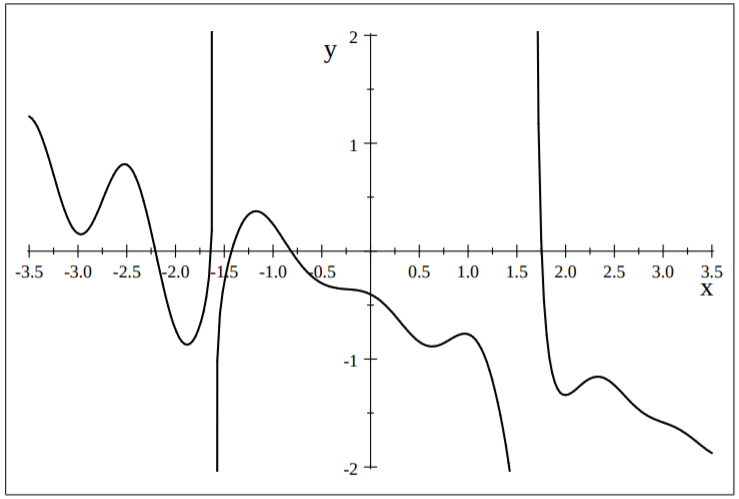
\includegraphics[scale=0.5]{images/grafica2.png}
\end{center}

\textbf{a)} A partir de esta gráfica estime (la estimación debe ser tan solo de la información de la gráfica y con dos cifras significativas) el valor de las raíces y ordénelas en forma ascendente: $\alpha_1 < \alpha_2 < \alpha_3 < \alpha_4 < \alpha_5$.

\begin{center}
$\alpha_i = $
\begin{tabular}{c c c c c}
    $\alpha_1$ & $\alpha_2$ & $\alpha_3$ & $\alpha_4$ & $\alpha_5$ \\
     %-2.24 & -1.62 & -1.48 & -0.76 & 1.75
     -2.2 & -1.6 & -1.4 & -0.76 & 1.7
\end{tabular}    
\end{center}

 Calcule $\beta_i = \lfloor \alpha \rfloor$ (la función Floor de
la estimación de la raíz iésima) y $\gamma_i = \lceil \alpha \rceil$ (la función Ceiling de la estimación
de la raíz iésima) para $i = 1, 2, 3, 4, 5$.


\begin{center}
$\beta_i = $
\begin{tabular}{c c c c c}
    $\lfloor \alpha_1 \rfloor$ & $\lfloor \alpha_2 \rfloor$ & $\lfloor \alpha_3 \rfloor$ & $\lfloor \alpha_4 \rfloor$ & $\lfloor \alpha_5 \rfloor$ \\
     %-2.24 & -1.62 & -1.48 & -0.76 & 1.75
     -3 & -2 & -2 & -1 & 1
\end{tabular}    
\end{center}

\begin{center}
$\gamma_i = $
\begin{tabular}{c c c c c}
    $\lceil \alpha_1 \rceil$ & $\lceil \alpha_2 \rceil$ & $\lceil \alpha_3 \rceil$ & $\lceil \alpha_4 \rceil$ & $\lceil \alpha_5 \rceil$ \\
     %-2.24 & -1.62 & -1.48 & -0.76 & 1.75
     -2 & -1 & -1 & 0 & 2
\end{tabular}    
\end{center}

En los casos en que se pueda, utilizar el método de bisección directamente para encontrar una aproximación de las raíces con 5 cifras significativas utilizando como intervalo inicial $[\beta_i,\gamma_i]$.

\begin{table}[H]
    \centering
    \begin{tabular}{|c|c|c|c|c|}
    \hline
it & $a$ & $b$ & $c$ & $f(c)$\\
\hline
0 & -3 & -2 & -2.5 & 0.80222222222\\
1 & -2.5 & -2 & -2.25 & 0.18085106383\\
2 & -2.25 & -2 & -2.125 & -0.32895925119\\
3 & -2.25 & -2.125 & -2.1875 & -0.076045641319\\
4 & -2.25 & -2.1875 & -2.21875 & 0.053498915288\\
5 & -2.21875 & -2.1875 & -2.203125 & -0.011198508772\\
6 & -2.21875 & -2.203125 & -2.2109375 & 0.021193949618\\
7 & -2.2109375 & -2.203125 & -2.20703125 & 0.0050055321585\\
8 & -2.20703125 & -2.203125 & -2.205078125 & -0.0030949264969\\
9 & -2.20703125 & -2.205078125 & -2.2060546875 & 0.00095574219219\\
10 & -2.2060546875 & -2.205078125 & -2.2055664062 & -0.0010694884246\\
11 & -2.2060546875 & -2.2055664062 & -2.2058105469 & -5.6846420121e-05\\
12 & -2.2060546875 & -2.2058105469 & -2.2059326172 & 0.00044945465556\\
13 & -2.2059326172 & -2.2058105469 & -2.205871582 & 0.00019630579817\\
14 & -2.205871582 & -2.2058105469 & -2.2058410645 & 6.9730107641e-05\\
\hline
\end{tabular}
    \caption{Tabla Método Bisección para $[\beta_1,\gamma_1]$}
    \label{tab:my_label}
\end{table}

\begin{table}[H]
\centering
\begin{tabular}{|c|c|c|c|c|}
\hline
it & $a$ & $b$ & $c$ & $f(c)$\\
\hline
0 & -2 & -1 & -1.5 & -0.28947368421\\
1 & -1.5 & -1 & -1.25 & 0.34081632653\\
2 & -1.5 & -1.25 & -1.375 & 0.14105260233\\
3 & -1.5 & -1.375 & -1.4375 & -0.037793666722\\
4 & -1.4375 & -1.375 & -1.40625 & 0.058854977196\\
5 & -1.4375 & -1.40625 & -1.421875 & 0.012445959988\\
6 & -1.4375 & -1.421875 & -1.4296875 & -0.012175377784\\
7 & -1.4296875 & -1.421875 & -1.42578125 & 0.00025709215321\\
8 & -1.4296875 & -1.42578125 & -1.427734375 & -0.0059283661149\\
9 & -1.427734375 & -1.42578125 & -1.4267578125 & -0.002827985111\\
10 & -1.4267578125 & -1.42578125 & -1.4262695312 & -0.0012835386646\\
11 & -1.4262695312 & -1.42578125 & -1.4260253906 & -0.000512746938\\
12 & -1.4260253906 & -1.42578125 & -1.4259033203 & -0.00012770839196\\
13 & -1.4259033203 & -1.42578125 & -1.4258422852 & 6.4721620897e-05\\
\hline
\end{tabular}
\caption{Tabla Método Bisección para $[\beta_2 ,\gamma_2]$}
\end{table}

Para el caso del intervalo $[\lfloor \alpha_2 \rfloor,\lceil \alpha_2 \rceil]$, los redondeos hacia arriba y hacia abajo son exactamente iguales que $[\lfloor \alpha_3 \rfloor,\lceil \alpha_3 \rceil]$, por lo que si bien el método ``funciona''(converge a una raíz) no le es posible tomar la raíz $\alpha_2$.

\begin{table}[H]
\centering
\begin{tabular}{|c|c|c|c|c|}
\hline
it & $a$ & $b$ & $c$ & $f(c)$\\
\hline
0 & -2 & -1 & -1.5 & -0.28947368421\\
1 & -1.5 & -1 & -1.25 & 0.34081632653\\
2 & -1.5 & -1.25 & -1.375 & 0.14105260233\\
3 & -1.5 & -1.375 & -1.4375 & -0.037793666722\\
4 & -1.4375 & -1.375 & -1.40625 & 0.058854977196\\
5 & -1.4375 & -1.40625 & -1.421875 & 0.012445959988\\
6 & -1.4375 & -1.421875 & -1.4296875 & -0.012175377784\\
7 & -1.4296875 & -1.421875 & -1.42578125 & 0.00025709215321\\
8 & -1.4296875 & -1.42578125 & -1.427734375 & -0.0059283661149\\
9 & -1.427734375 & -1.42578125 & -1.4267578125 & -0.002827985111\\
10 & -1.4267578125 & -1.42578125 & -1.4262695312 & -0.0012835386646\\
11 & -1.4262695312 & -1.42578125 & -1.4260253906 & -0.000512746938\\
12 & -1.4260253906 & -1.42578125 & -1.4259033203 & -0.00012770839196\\
13 & -1.4259033203 & -1.42578125 & -1.4258422852 & 6.4721620897e-05\\
\hline
\end{tabular}
\caption{Tabla Método Bisección para $[\beta_3 ,\gamma_3]$}
\end{table}

\begin{table}[H]
\centering
\begin{tabular}{|c|c|c|c|c|}
\hline
it & $a$ & $b$ & $c$ & $f(c)$\\
\hline
0 & -1 & 0 & -0.5 & -0.2972027972\\
1 & -1 & -0.5 & -0.75 & -0.084178498986\\
2 & -1 & -0.75 & -0.875 & 0.082494183321\\
3 & -0.875 & -0.75 & -0.8125 & -0.003771670383\\
4 & -0.875 & -0.8125 & -0.84375 & 0.038917494974\\
5 & -0.84375 & -0.8125 & -0.828125 & 0.017421756859\\
6 & -0.828125 & -0.8125 & -0.8203125 & 0.006782591065\\
7 & -0.8203125 & -0.8125 & -0.81640625 & 0.0014942871157\\
8 & -0.81640625 & -0.8125 & -0.814453125 & -0.0011415535443\\
9 & -0.81640625 & -0.814453125 & -0.8154296875 & 0.00017565982032\\
10 & -0.8154296875 & -0.814453125 & -0.81494140625 & -0.00048312467133\\
11 & -0.8154296875 & -0.81494140625 & -0.81518554688 & -0.00015377674459\\
12 & -0.8154296875 & -0.81518554688 & -0.81530761719 & 1.0930474775e-05\\
13 & -0.81530761719 & -0.81518554688 & -0.81524658203 & -7.1425902764e-05\\
14 & -0.81530761719 & -0.81524658203 & -0.81527709961 & -3.0248405699e-05\\
15 & -0.81530761719 & -0.81527709961 & -0.8152923584 & -9.6591383556e-06\\
\hline
\end{tabular}
\caption{Tabla Método Bisección para $[\beta_4,\gamma_4]$}
\end{table}

\begin{table}[H]
\centering
    \begin{tabular}{|c|c|c|c|c|}
    \hline
it & a & b & c & f(c) \\ 
\hline
\end{tabular}
\caption{Tabla Método Bisección para $[\beta_5,\gamma_5]$}
\end{table}

Para el caso del intervalo $[\lfloor \alpha_5 \rfloor,\lceil \alpha_5 \rceil]$ en la primera iteración de bisección, toma como punto central a 1.5, valor donde en la función se indetermina, por lo que no es posible aplicar el método de la bisección.

Notará que el método de bisección falla en algunos casos, explique el porqué de esta situación. En estos casos, alterar tan solo un extremo del intervalo inicial al intercambiar el valor de $\beta_i$ o de $\gamma_i$ por $\alpha_i \pm 0.05$ (i.e. según sea el caso se intercambia ya sea $\beta_i$ por $\alpha_i - 0.05$ o $\gamma_i$ por $\alpha_i + 0.05$). Después de este proceso se tendrán estimaciones a las raíces $b_1,b_2,b_3,b_4$ y $b_5$ correctas a 5 cifras.

\begin{table}[H]
\centering
\begin{tabular}{|c|c|c|c|c|}
\hline
it & $a$ & $b$ & $c$ & $f(c)$\\
\hline
0 & -2 & -1.6 & -1.8 & -0.79876990751\\
1 & -1.8 & -1.6 & -1.7 & -0.50916595582\\
2 & -1.7 & -1.6 & -1.65 & -0.17696082432\\
3 & -1.65 & -1.6 & -1.625 & 0.28642510539\\
4 & -1.65 & -1.625 & -1.6375 & -0.010308427494\\
5 & -1.6375 & -1.625 & -1.63125 & 0.11211302339\\
6 & -1.6375 & -1.63125 & -1.634375 & 0.046177460444\\
7 & -1.6375 & -1.634375 & -1.6359375 & 0.016906434128\\
8 & -1.6375 & -1.6359375 & -1.63671875 & 0.0030582700191\\
9 & -1.6375 & -1.63671875 & -1.637109375 & -0.0036833763396\\
10 & -1.637109375 & -1.63671875 & -1.6369140625 & -0.0003273570324\\
11 & -1.6369140625 & -1.63671875 & -1.6368164063 & 0.0013617263081\\
12 & -1.6369140625 & -1.6368164063 & -1.6368652344 & 0.0005162557679\\
13 & -1.6369140625 & -1.6368652344 & -1.6368896484 & 9.4217607685e-05\\
14 & -1.6369140625 & -1.6368896484 & -1.6369018555 & -0.00011662759533\\
15 & -1.6369018555 & -1.6368896484 & -1.636895752 & -1.1219471693e-05\\
16 & -1.636895752 & -1.6368896484 & -1.6368927002 & 4.1495447638e-05\\
17 & -1.636895752 & -1.6368927002 & -1.6368942261 & 1.5137082998e-05\\
18 & -1.636895752 & -1.6368942261 & -1.636894989 & 1.9585794183e-06\\
\hline
\end{tabular}
\caption{Tabla Método Bisección para $[\beta_2, \alpha_2 +0.05]$}
\end{table}

Tabla Método Bisección para $[\lfloor \alpha_5 \rfloor, \alpha_5 +0.05]$, no converge ya que el intervalo $[\lfloor \alpha_5 \rfloor, \alpha_5 +0.05]$ no es continuo.

Tabla Método Bisección para $[\alpha_5 - 0.05,\lceil \alpha_5 \rceil]$, no converge ya que el intervalo $[\alpha_5 - 0.05,\lceil \alpha_5 \rceil]$ no es continuo.
%%%%%%%%%%%%%%%%%%%%%%%%%%%%%%%%%%%%%%%%%%%%%%%%%%%%%%%%%%%%%%%%%%%%%%%%%%%%%%%%%%%%%%%%

\textbf{b)} En los casos en que se pueda, estime el valor de las raíces con 14 cifras significativas utilizando el método de Newton con la derivada analítica de $f(x)$. Mostrar en una sola tabla los resultados de cada iteración del método para las siguientes condiciones iniciales:

\begin{enumerate}[i]
    \item Los valores iniciales de $\beta_i$
    \item Los valores iniciales de $\gamma_i$
    \item Los valores iniciales de $\alpha_i$
    \item Los valores iniciales de $b_i$
\end{enumerate}

Al final para cada raíz se debe reportar una tabla de este tipo:

\begin{table}[H]
    \centering
    \begin{tabular}{|c|c|c|c|c|c|c|c|c|c|}
\hline
     &  \multicolumn{9}{|c|}{Condición Inicial}\\
     \hline
     & \multicolumn{3}{|c|}{$\beta_i$} & \multicolumn{2}{|c|}{$\gamma_i$} & \multicolumn{2}{|c|}{$\alpha_i$} & \multicolumn{2}{|c|}{$b_i$}\\
     \hline
     Iteración & $x_k$ & $f_k$ & $|x_{k+1}-x_k|$ & $x_k$ & $\ldots$ & $x_k$ & $\ldots$ & $x_k$ & $\ldots$ \\
     \hline
     0&$x_0=\beta_i$&$f_0$&$|x_1 - x_0|$&$x_0=\gamma_i$&\ldots&$x_0=\alpha_i$&\ldots&$x_0=b_i$&\ldots\\
     \hline
     1&$x_1=\beta_i$&$f_1$&$|x_2 - x_1|$&$x_1=\gamma_i$&\ldots&$x_1=\alpha_i$&\ldots&$x_1=b_i$&\ldots\\
     \hline
     2&$x_2=\beta_i$&$f_2$&$|x_2 - x_1|$&$x_2=\gamma_i$&\ldots&$x_2=\alpha_i$&\ldots&$x_2=b_i$&\ldots\\
     \hline
     $\vdots$ & $\vdots$ & $\vdots$ & $\vdots$ & $\vdots$ & $\ddots$ &$ \vdots$ &$ \ddots$ & $\vdots$ & $\ddots$ \\
     \hline
\end{tabular}
\end{table}

\subsection*{Tablas Ejercicio 3 Método de Newton}
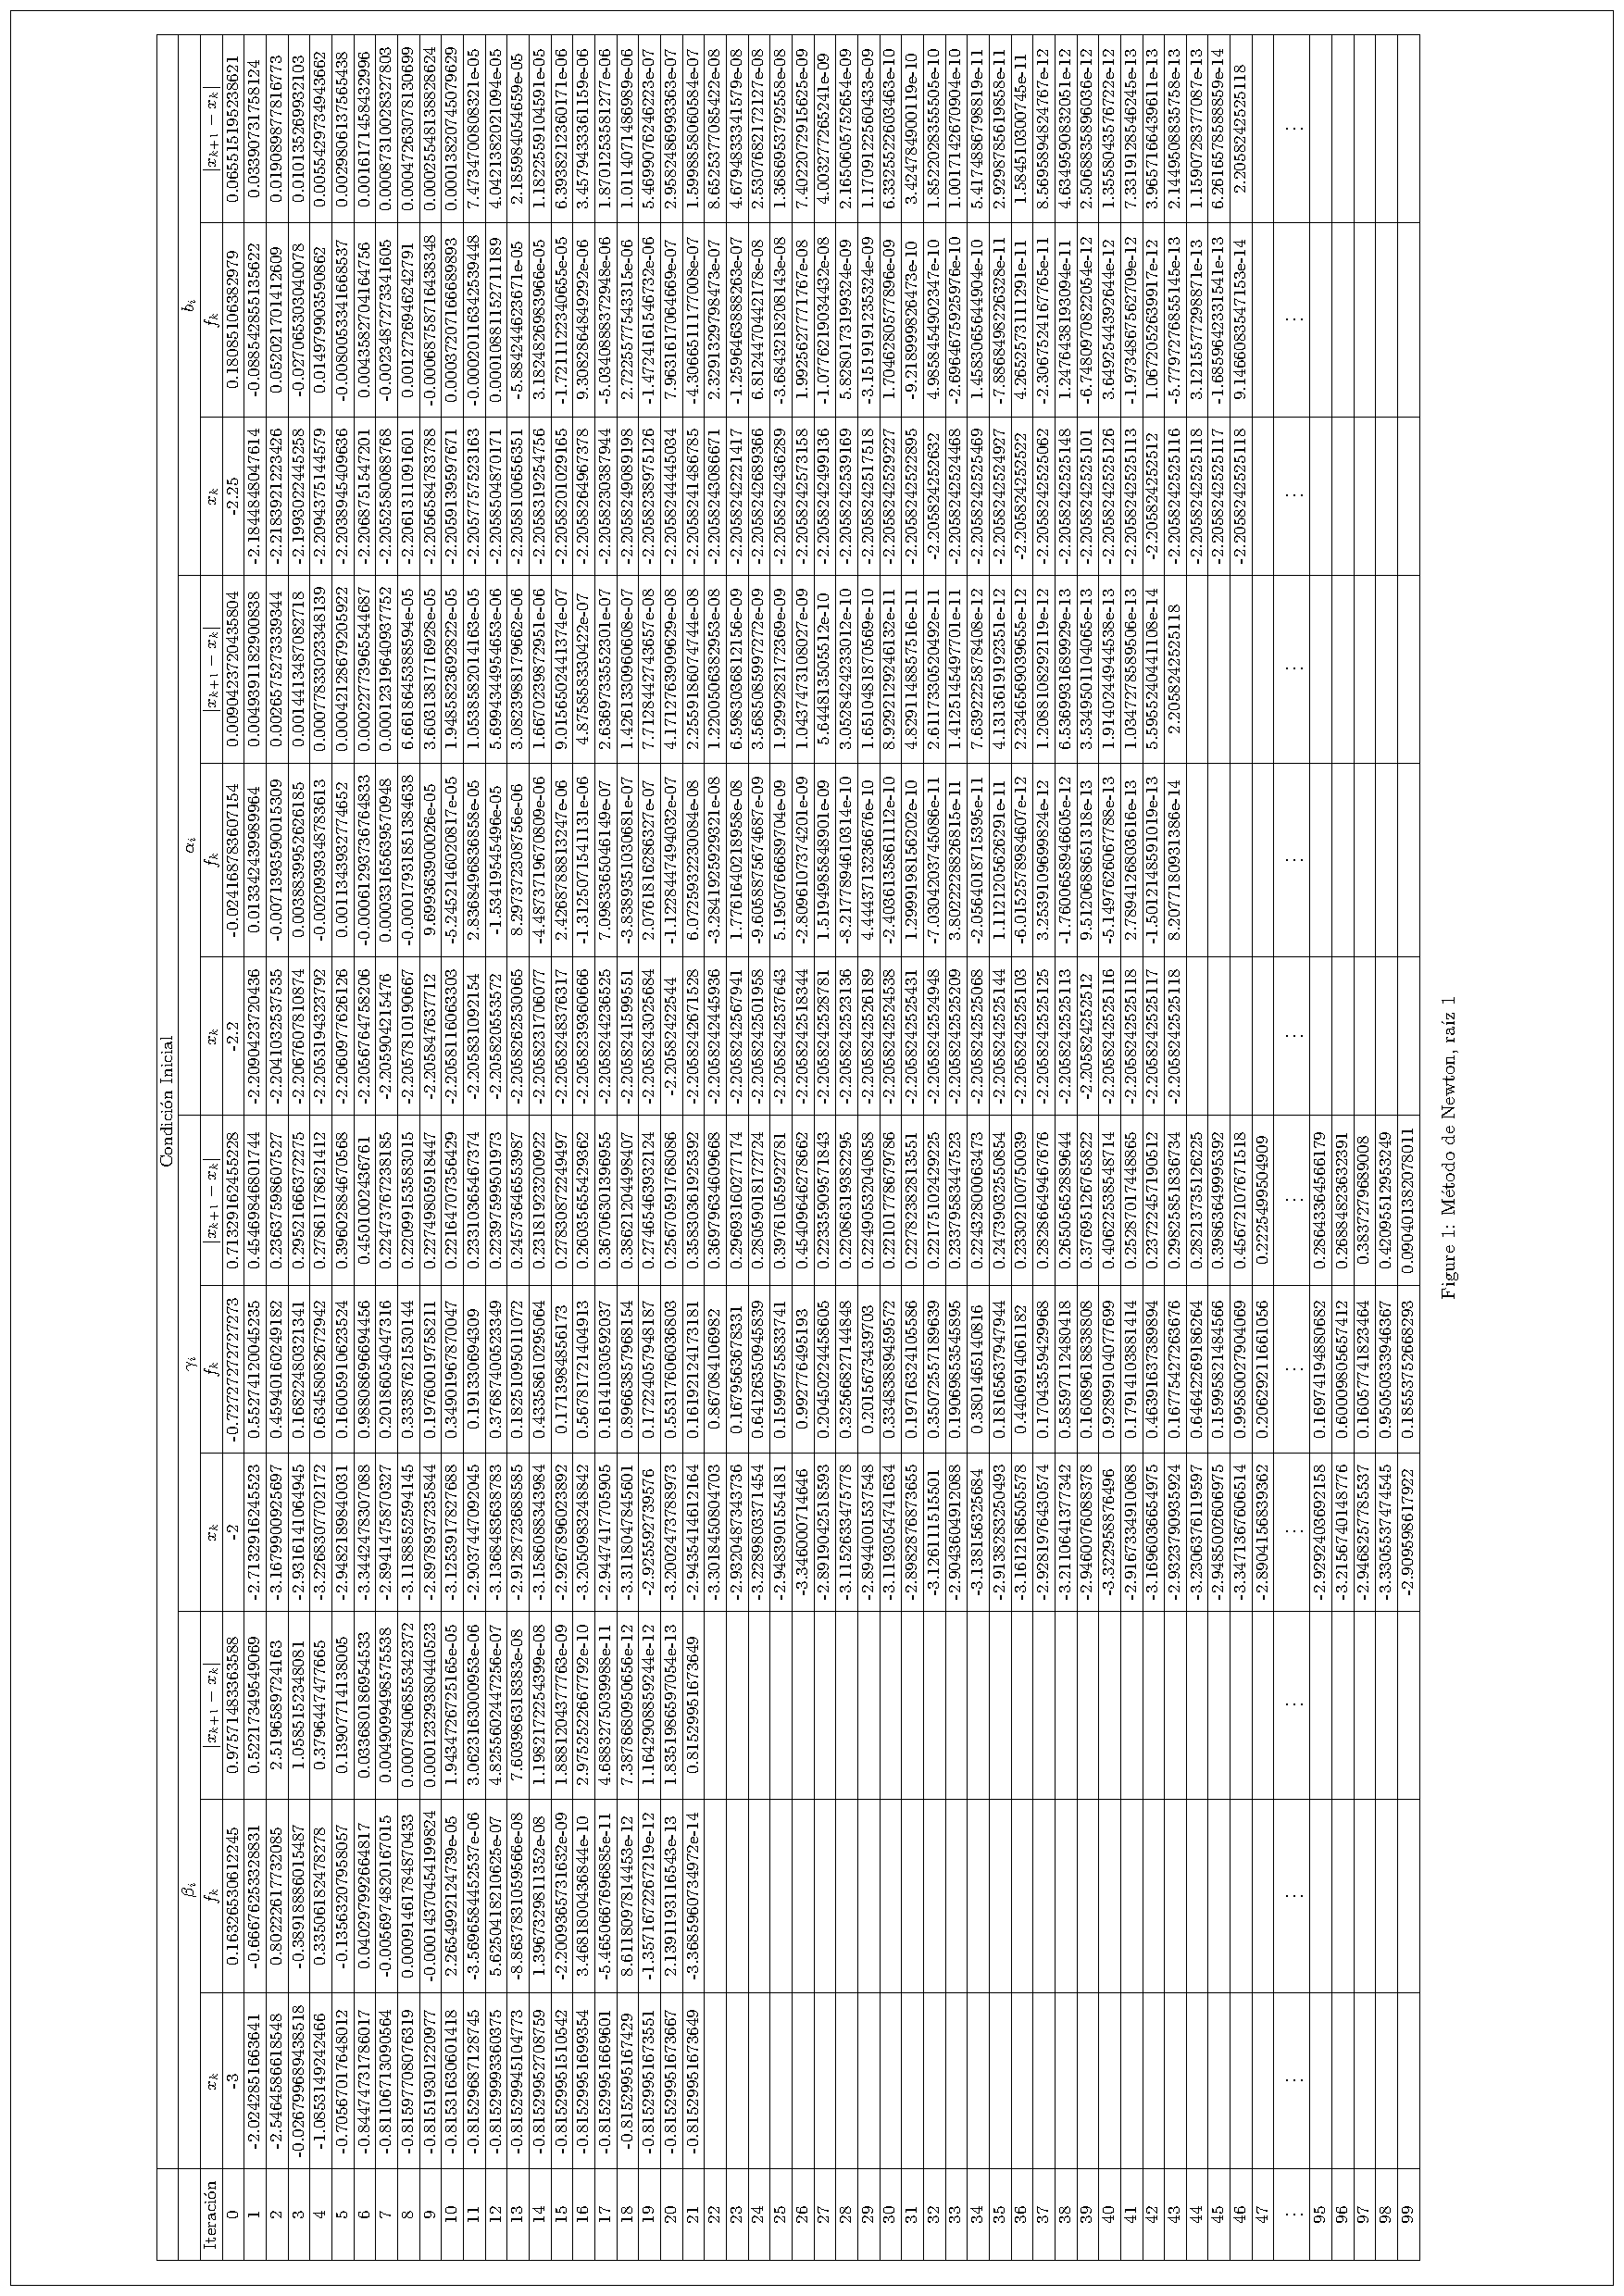
\includepdf[pages=-]{pdfs/newtons.pdf}

\textbf{c.} Repita el ejercicio anterior utilizando el método de la secante con los siguientes pares de condiciones iniciales:

\begin{enumerate}
    \item Los valores de $\beta_i$ y $\gamma_i$.
    \item Los valores de $\beta_i$ y $\alpha_i$.
    \item Los valores de $\alpha_i$ y $\gamma_i$.
    \item Los valores de $\beta_i$ y $b_i$.
    \item Los valores de $b_i$ y $\gamma_i$.
\end{enumerate}

\subsection*{Tablas Ejercicio 3 Método de la Secante}
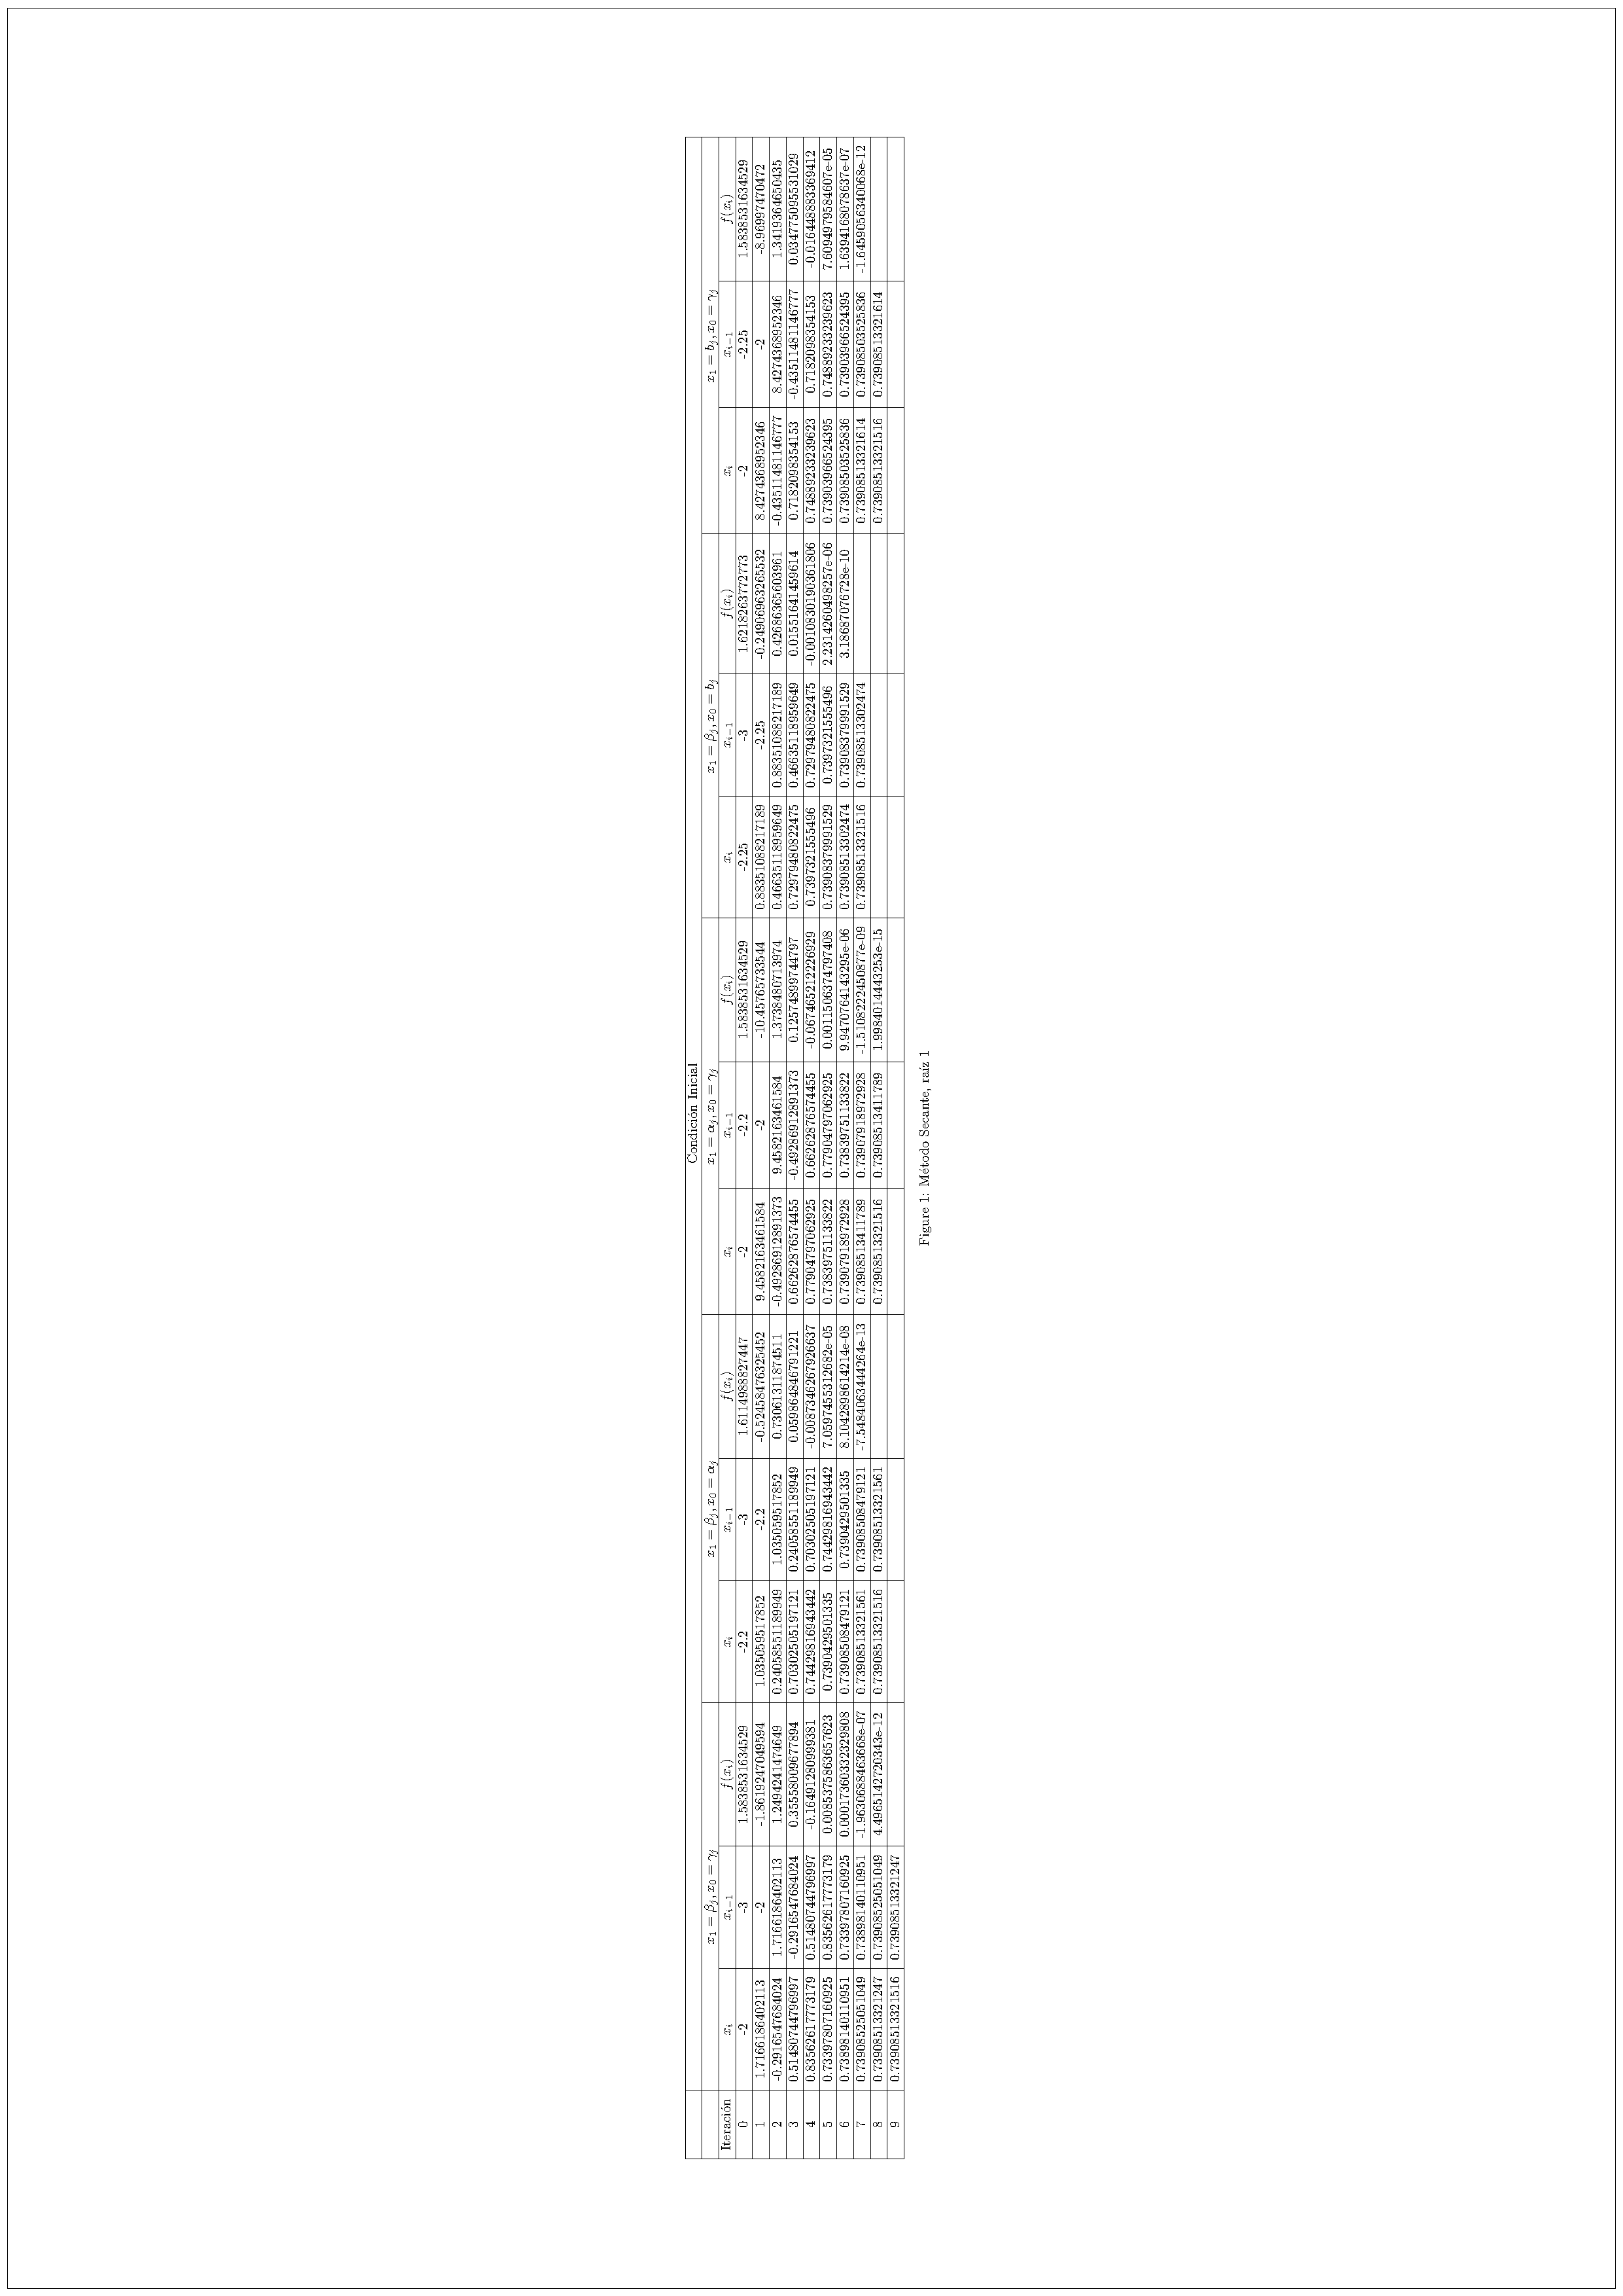
\includepdf[pages=-]{pdfs/secantes.pdf}

\textbf{d.} Repita el ejercicio anterior utilizando el método de Muller con las siguientes tercias de condiciones iniciales:

\begin{enumerate}
    \item Los valores de $\beta_i$, $\alpha_i$ $\gamma_i$.
    \item Los valores de $\beta_i$, $b_i$ $\gamma_i$.
    \item Los valores de $\beta_i$, $\alpha_i$ $b_i$.
    \item Los valores de $\alpha_i$, $b_i$ $\gamma_i$.
\end{enumerate}


\subsection*{Tablas Ejercicio 3 Método de Muller}
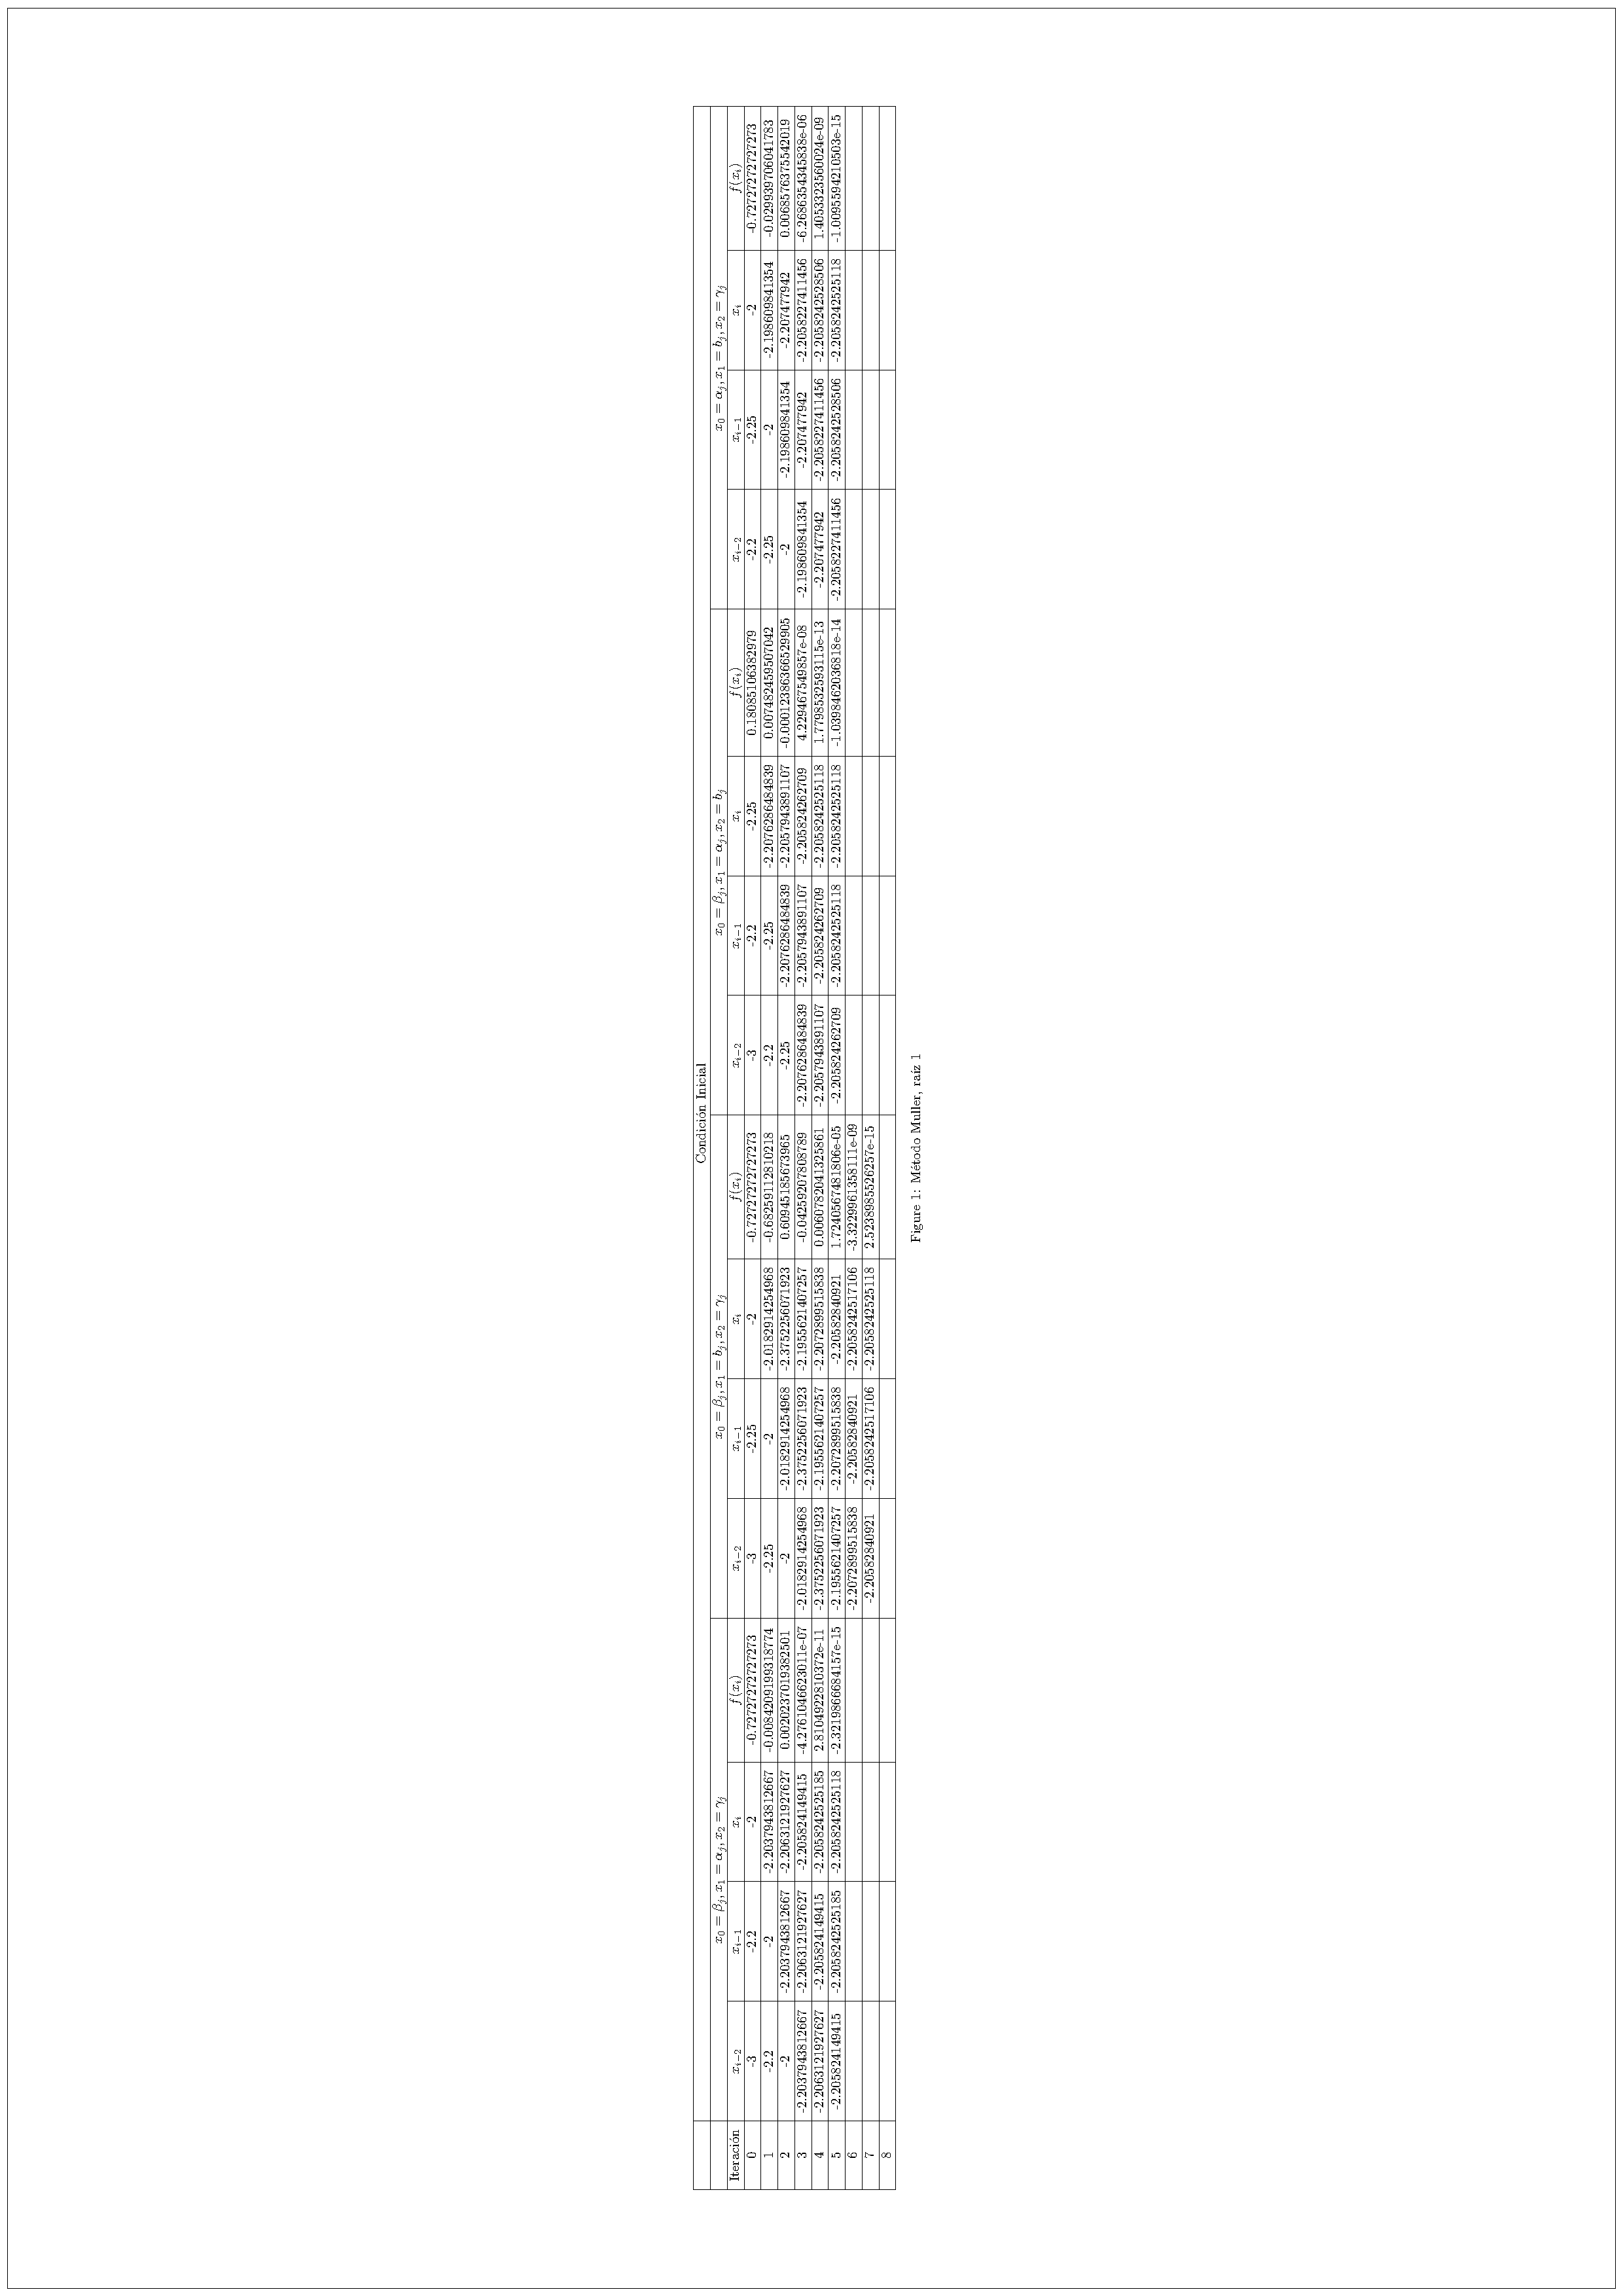
\includepdf[pages=-]{pdfs/mullers.pdf}

\subsection*{Derivada analítica de la función $f(x)$}

\begin{gather*}
    f'(x) = \frac{d}{dx} \frac{(\cos{(2\pi x)}-6)x^3}{15x^2-x-40} - \frac{d}{dx} \frac{(2\cos{(2\pi x)}+7)x^2}{15x^2-x-40} - \frac{d}{dx} \frac{2(\cos{(2\pi x)}-10)x}{15x^2-x-40} - \frac{d}{dx} \frac{3\cos{(2\pi x)}}{15x^2-x-40}\\
    + \frac{d}{dx} \frac{19}{15x^2-x-40}
\end{gather*}

\begin{gather*}
    \frac{d}{dx} \frac{(\cos{(2\pi x)}-6)x^3}{15x^2-x-40} = \frac{d}{dx} \frac{(\cos{(2\pi x)}-6)x^3}{15x^2-x-40} - \frac{d}{dx} \frac{-6x^3}{15x^2-x-40}\\
    \frac{d}{dx} \frac{(\cos{(2\pi x)}-6)x^3}{15x^2-x-40}
    = \frac{((-2\pi \sin{(2\pi x)}x^3 + 3\cos{(2\pi x)x^2})(15x^2-x-40))-(30x-1)(\cos{(2\pi x)}x^3)}{(15x^2 -x-40)^2}\\
    = \frac{-30\pi\sin{(2\pi x)}x^5 + 2\pi\sin{(2\pi x)}x^4 + 15\pi\cos{(2\pi x)x^4} + 80\pi\sin{(2\pi x)}x^3 -2\cos{(2\pi x)}x^3 - 120\cos{(2\pi x)}x^2}{(15x^2-x-40)^2}\\
    \frac{d}{dx} \frac{-6x^3}{15x^2-x-40} = \frac{-18x^2(15x^2-x-40) - (30x-1)(-6x^3)}{(15x^2-x-40)^2}\\
    = \frac{-270x^4 + 18x^3 + 720x^2 + 180x^4 - 6x^3}{(15x^2-x-40)^2}\\
    = \frac{-90x^4 + 12x^3 + 720x^2}{(15x^2-x-40)^2}\\
    \frac{d}{dx} \frac{(\cos{(2\pi x)}-6)x^3}{15x^2-x-40} = \frac{-30\pi\sin{(2\pi x)}x^5 + 2\pi\sin{(2\pi x)}x^4 + 15\pi\cos{(2\pi x)x^4} -90x^4 + 80\pi\sin{(2\pi x)}x^3 }{(15x^2-x-40)^2}\\
    + \frac{-2\cos{(2\pi x)}x^3 +12x^3 - 120\cos{(2\pi x)}x^2 + 720x^2}{(15x^2-x-40)^2}
\end{gather*}

\begin{gather*}
    \frac{d}{dx} - \frac{(2\cos{(2\pi x)}+7)x^2}{15x^2-x-40} = \frac{d}{dx} \frac{-2\cos{(2\pi x)}x^2}{15x^2-x-40} - \frac{d}{dx} \frac{7x^2}{15x^2-x-40}\\
    \frac{d}{dx} \frac{-2\cos{(2\pi x)}x^2}{15x^2-x-40} = \frac{(4\sin{(2\pi x)}x^2 - 4\cos{(2\pi x)}x)(15x^2-x-40) - (30x-1)(-2\cos{(2\pi x)}x^2)}{(15x^2-x-40)^2}\\
    = \frac{(60\sin{(2\pi x)}x^4 -4\sin{(2\pi x)}x^3 -160\sin{(2\pi x)}x^2 - 60\cos{(2\pi x)}x^3 + 4\cos{(2\pi x)}x^2 + 160\cos{(2\pi x)}x)}{(15x^2-x-40)^2}\\
    + \frac{(60\cos{(2\pi x)}x^3 -2\cos{(2\pi x)}x^2)}{(15x^2-x-40)^2}\\
    = \frac{60\sin{(2\pi x)}x^4 - 4\sin{(2\pi x)}x^3 - 160\sin{(2\pi x)}x^2 + 2\cos{(2\pi x)}x^2 + 160\cos{(2\pi x)}x}{(15x^2-x-40)^2}\\
    \frac{d}{dx} \frac{7x^2}{15x^2-x-40} = \frac{14x(15x^2-x-40)-(30x-1)(7x^2)}{(15x^2-x-40)^2}\\
    = \frac{-7x^2-560x}{(15x^2-x-40)^2}\\
    \frac{d}{dx} - \frac{(2\cos{(2\pi x)}+7)x^2}{15x^2-x-40} = \frac{60\sin{(2\pi x)}x^4 - 4\sin{(2\pi x)}x^3 - 160\sin{(2\pi x)}x^2 + 2\cos{(2\pi x)}x^2}{(15x^2-x-40)^2}\\
    + \frac{7x^2 + 160\cos{(2\pi x)}x + 560x}{(15x^2-x-40)^2}  
\end{gather*}

\begin{gather*}
    \frac{d}{dx} \frac{-2(\cos{(2\pi x)}-10)x}{15x^2-x-40} = \frac{d}{dx} \frac{-2\cos{(2\pi x)}x}{15x^2-x-40} + \frac{d}{dx} \frac{20x}{15x^2-x-40}\\
    \frac{d}{dx} \frac{-2\cos{(2\pi x)}x}{15x^2-x-40} = \frac{(4\pi \sin{(2\pi x)}x-2\cos{(2\pi x)})(15x^2 -x-40)+60\cos{(2\pi x)}x^2-2\cos{(2\pi x)}x}{(15x^2-x-40)^2}\\
    = \frac{60\pi\sin{(2\pi x)}x^3 - 4\pi\sin{(2\pi x)}x^2 +30\cos{(2\pi x)}x^2 -160\pi\sin{(2\pi x)}x +80\cos{(2\pi x)}}{(15x^2-x-40)^2}\\
    \frac{d}{dx} \frac{20x}{15x^2-x-40} = \frac{20(15x^2 -x-40)-(30x-1)(20x)}{(15x^2-x-40)^2}\\
    = \frac{-300x^2 -800}{(15x^2-x-40)^2}\\
    \frac{d}{dx} \frac{-2(\cos{(2\pi x)}-10)x}{15x^2-x-40} = \frac{60\pi\sin{(2\pi x)}x^3 - 4\pi\sin{(2\pi x)}x^2 +30\cos{(2\pi x)}x^2 -300x^2}{(15x^2-x-40)^2}\\
     + \frac{-160\pi\sin{(2\pi x)}x +80\cos{(2\pi x)} -800}{(15x^2-x-40)^2}
\end{gather*}

\begin{gather*}
    \frac{d}{dx} \frac{-3\cos{(2\pi x)}}{15x^2-x-40} = \frac{(6\pi\sin{(2\pi x)})(15x^2-x-40)-(30x-1)(-3\cos{(2\pi x)})}{(15x^2-x-40)^2}\\
    = \frac{90\pi\sin{(2\pi x)}x^2 -6\pi\sin{(2\pi x)}x + 90\cos{(2\pi x)}x - 240\pi\sin{(2\pi x)} -3\cos{(2\pi x)}}{(15x^2-x-40)^2}
\end{gather*}

\begin{gather*}
    \frac{d}{dx} \frac{19}{15x^2-x-40}=\frac{-570x+19}{(15x^2-x-40)^2}
\end{gather*}


%%%%%%%%%%%%%%%%%%%%%%%%%%%%%%%%%%%%%%%%

\newpage
\section*{Ejercicio 4}
\textbf{4.} Considere el siguiente polinomio de grado 9

\begin{equation*}
    P(x) = 756x^9 + 2448x^8 + 1605x^7 -2583x^6 -4705x^5 -2069x^4 +1643x^3 +1773x^2 -20x -300
\end{equation*}

\textbf{a.} Tabule los valores de $P(x)$ en el intervalo $[-4,4]$ para los puntos

\begin{equation*}
    x_k = -4+\frac{k}{10}, k=0,1,2,\ldots,80
\end{equation*}

evaluando directamente el polinomio en esos puntos y luego con la regla de Horner.

\begin{center}
\begin{tabular}{|c|c|c|c|}
\hline
it & $x_k$ & $f(x_k)$ & $h(x_k)$\\
\hline
0 & -4 & -7.04138e+07 & -7.04138e+07\\
1 & -3.9 & -5.42003e+07 & -5.42003e+07\\
2 & -3.8 & -4.13785e+07 & -4.13785e+07\\
3 & -3.7 & -3.13137e+07 & -3.13137e+07\\
4 & -3.6 & -2.34751e+07 & -2.34751e+07\\
5 & -3.5 & -1.74217e+07 & -1.74217e+07\\
6 & -3.4 & -1.27891e+07 & -1.27891e+07\\
7 & -3.3 & -9.27834e+06 & -9.27834e+06\\
8 & -3.2 & -6.64569e+06 & -6.64569e+06\\
9 & -3.1 & -4.694e+06 & -4.694e+06\\
10 & -3 & -3.26508e+06 & -3.26508e+06\\
11 & -2.9 & -2.23309e+06 & -2.23309e+06\\
12 & -2.8 & -1.49889e+06 & -1.49889e+06\\
13 & -2.7 & -985170 & -985170\\
14 & -2.6 & -632323 & -632323\\
15 & -2.5 & -394977 & -394977\\
16 & -2.4 & -239066 & -239066\\
17 & -2.3 & -139404 & -139404\\
18 & -2.2 & -77697.4 & -77697.4\\
19 & -2.1 & -40916.8 & -40916.8\\
20 & -2 & -19992 & -19992\\
21 & -1.9 & -8773.96 & -8773.96\\
22 & -1.8 & -3222.69 & -3222.69\\
23 & -1.7 & -782.902 & -782.902\\
24 & -1.6 & 86.6898 & 86.6898\\
25 & -1.5 & 259.875 & 259.875\\
26 & -1.4 & 190.943 & 190.943\\
27 & -1.3 & 86.0656 & 86.0656\\
28 & -1.2 & 16.6393 & 16.6393\\
\end{tabular}
\end{center}

\begin{center}
\begin{tabular}{|c|c|c|c|}
29 & -1.1 & -10.0124 & -10.0124\\
30 & -1 & -10 & -10\\
31 & -0.9 & -2.31724 & -2.31724\\
32 & -0.8 & -0.697203 & -0.697203\\
33 & -0.7 & -12.2276 & -12.2276\\
34 & -0.6 & -38.8335 & -38.8335\\
35 & -0.5 & -79.2188 & -79.2188\\
36 & -0.4 & -130.063 & -130.063\\
37 & -0.3 & -186.205 & -186.205\\
38 & -0.2 & -240.209 & -240.209\\
39 & -0.1 & -282.076 & -282.076\\
40 & 0 & -300 & -300\\
41 & 0.1 & -282.883 & -282.883\\
42 & 0.2 & -224.89 & -224.89\\
43 & 0.3 & -131.618 & -131.618\\
44 & 0.4 & -26.4614 & -26.4614\\
45 & 0.5 & 45.5 & 45.5\\
46 & 0.6 & 20.3178 & 20.3178\\
47 & 0.7 & -169.296 & -169.296\\
48 & 0.8 & -557.611 & -557.611\\
49 & 0.9 & -1078.22 & -1078.22\\
50 & 1 & -1452 & -1452\\
51 & 1.1 & -1014.65 & -1014.65\\
52 & 1.2 & 1535.35 & 1535.35\\
53 & 1.3 & 8491.01 & 8491.01\\
54 & 1.4 & 23619.7 & 23619.7\\
55 & 1.5 & 52805.2 & 52805.2\\
56 & 1.6 & 104883 & 104883\\
57 & 1.7 & 192708 & 192708\\
58 & 1.8 & 334503 & 334503\\
59 & 1.9 & 555524 & 555524\\
60 & 2 & 890120 & 890120\\
61 & 2.1 & 1.38422e+06 & 1.38422e+06\\
62 & 2.2 & 2.09833e+06 & 2.09833e+06\\
63 & 2.3 & 3.11112e+06 & 3.11112e+06\\
64 & 2.4 & 4.52365e+06 & 4.52365e+06\\
65 & 2.5 & 6.46437e+06 & 6.46437e+06\\
66 & 2.6 & 9.09491e+06 & 9.09491e+06\\
67 & 2.7 & 1.26168e+07 & 1.26168e+07\\
68 & 2.8 & 1.72795e+07 & 1.72795e+07\\
69 & 2.9 & 2.33888e+07 & 2.33888e+07\\
70 & 3 & 3.13179e+07 & 3.13179e+07\\
71 & 3.1 & 4.1518e+07 & 4.1518e+07\\
72 & 3.2 & 5.45326e+07 & 5.45326e+07\\
73 & 3.3 & 7.10117e+07 & 7.10117e+07\\
74 & 3.4 & 9.17285e+07 & 9.17285e+07\\
\end{tabular}
\end{center}

\begin{center}
\begin{tabular}{|c|c|c|c|}
75 & 3.5 & 1.17599e+08 & 1.17599e+08\\
76 & 3.6 & 1.49702e+08 & 1.49702e+08\\
77 & 3.7 & 1.89303e+08 & 1.89303e+08\\
78 & 3.8 & 2.3788e+08 & 2.3788e+08\\
79 & 3.9 & 2.97153e+08 & 2.97153e+08\\
80 & 4 & 3.69115e+08 & 3.69115e+08\\
\hline
\end{tabular}
\end{center}

\textbf{b.} Utilizando los métodos vistos en clase(regla de signos de Descartes y cotas para raíces) extraiga toda la información posible sobre las 9 raíces del polinomio $P(x)=0$

Información obtenida por Regla de signos de Descartes: El polinomio $P(x)$ tiene 3 cambios de signo, por lo que tendrá 3 o 1 raíz real positiva, El polinomio $P(-x)$ tiene 6 cambios de signo, por lo que tendrá 6, 4, 2 o 0 raíces reales negativas y 0 o 4 raíces complejas según sea el caso.

\begin{center}
\begin{tabular}{|c|c|c|c|}
\hline
Pos & Neg & Im & Total \\
\hline
3 & 6 & 0 & 9\\
\hline
3 & 4 & 2 & 9\\
\hline
3 & 2 & 4 & 9\\
\hline
3 & 0 & 6 & 9\\
\hline
1 & 6 & 2 & 9\\
\hline
1 & 4 & 4 & 9\\
\hline
1 & 2 & 6 & 9\\
\hline
1 & 0 & 8 & 9\\
\hline
\end{tabular}
\end{center}

Información obtenida por Cotas para raíces: Al calcular $p_1$ y $p_2$ para determinar $R_1$ se encontró que el mínimo fue el caso $p_2$ con un valor de $R1= p_2 = 0.9024017729792827$ y en el caso para determinar el valor de $R_2$ el máximo de los casos fue $|\frac{a_5}{a_n}|$ con un valor de $R_2 = 7.223544973544974$

\textbf{c)} Utilizando tan solo la información proveniente de los incisos anteriores, encuentre todas las raíces del polinomio con 13 cifras significativas utilizando:

\begin{enumerate}
    \item El método de Newton para encontrar una raíz y ``desinflando" el polinomio para encontrar la siguiente y así sucesivamente hasta llegar a un polinomio en donde pueda estimar la raíz analíticamente. Si es necesario utilice números complejos para encontrar las raíces.
    \item El método de Baristrow pero ahora encontrando un par de raíces y ``desinflando'' el polinomio para encontrar el siguiente par y así sucesivamente hasta llegar a un polinomio en donde pueda estimar la raíz analíticamente.
\end{enumerate}

\subsection*{Raíces por método de Newton}

Con $x_0 = 0.9$ (por el análisis de cotas) 

\begin{table}[H]
\centering
\begin{tabular}{|c|c|c|}
\hline
it & $x_i$ & $f(x_i)$\\
\hline
0 & 0.9 & -1078.221308736\\
1 & 0.69220520726789 & -147.41583925486\\
2 & 0.63814154242187 & -29.479628343535\\
3 & 0.62029759744309 & -2.9514324204214\\
4 & 0.61806854176472 & -0.044366270043668\\
5 & 0.61803399701092 & -1.0604663714275e-05\\
6 & 0.6180339887499 & -7.389644451905e-13\\
\hline
\end{tabular}
\caption{Raíz 1, método de Newton}
\end{table}

ahora con la raíz 1 $r_1 = 0.6180339887499$, desinflando el polinomio obtengo:
\begin{equation*}
Q_{n-1}(x) = 756.000000x^8 + 2915.233695x^7 + 3406.713509x^6-477.535262x^5
\end{equation*}
\begin{equation*}
-5000.133022x^4 -5159.252156x^3 -1545.593189x^2 + 817.770876x + 485.410197
\end{equation*}
y su derivada
\begin{equation*}
Q_{n-1}'(x) = 6048x^7 + 20406.635868464x^6 + 20440.281053789x^5 -2387.6763076316x^4
\end{equation*}
\begin{equation*}
-20000.532089799x^3 -15477.756468434x^2 -3091.1863780573x + 817.77087639997
\end{equation*}

Con $x_0 = 7.2$ (por el análisis de cotas) 
\begin{table}[H]
\centering
\begin{tabular}{|c|c|c|}
\hline
it & $x_i$ & $f(x_i)$\\
\hline
0 & 7.2 & 8833947864.5231\\
\hline
1 & 6.2491155490969 & 3032535388.7643\\
2 & 5.4186873991915 & 1040637595.2714\\
3 & 4.6939893278164 & 356917065.2372\\
4 & 4.0622280453408 & 122322283.73574\\
5 & 3.5123364179505 & 41874853.261848\\
6 & 3.0348092522332 & 14310450.049406\\
7 & 2.6215859865174 & 4877313.0982098\\
8 & 2.265990725388 & 1655019.4597158\\
9 & 1.9627505431414 & 557428.43949526\\
10 & 1.7081304746031 & 185241.99827423\\
11 & 1.5002444306906 & 59963.265306361\\
12 & 1.3395642302432 & 18332.373958553\\
13 & 1.2291466076913 & 4865.2385435735\\
14 & 1.1714989407442 & 872.07388053915\\
15 & 1.1557768478462 & 52.388554271875\\
16 & 1.154705292803 & 0.2303976019532\\
17 & 1.1547005384725 & 4.5190610080681e-06\\
18 & 1.1547005383793 & -5.4569682106376e-12\\
98 & 1.1547005383793 & -5.4569682106376e-12\\
99 & 1.1547005383793 & 5.7411853049416e-12\\
\hline
\end{tabular}
\caption{Raíz 2, método de Newton}
\end{table}

con $r_2 = 1.1547005383793$, y desinflando el polinomio nuevamente obtengo:

\begin{equation*}
    Q_{n-2}(x) = 756.000000x^7 3788.187303x^6 7780.935427x^5 8507.115065x^4 4823.037323x^3 409.911637x^2
\end{equation*}
\begin{equation*}
     -1072.268001x -420.377562
\end{equation*}

Derivada de $Q_{n-2}(x)$
\begin{equation*}
    Q_{n-2}'(x) = 42336.000000x^6 + 122439.815211x^5 + 102201.405269x^4 -9550.705231x^3 -60001.596269x^2
\end{equation*}
\begin{equation*}
    -30955.512937x -3091.186378
\end{equation*}

Con $x_0 = 7.2$ (por el análisis de cotas) 
\begin{table}[H]
\centering
\begin{tabular}{|c|c|c|}
\hline
it & $x_i$ & $f(x_i)$\\
\hline
0 & 7.2 & 1461292020.4543\\
1 & 6.0716307471977 & 496601829.8902\\
2 & 5.1049113924499 & 168746600.21953\\
3 & 4.2768572957628 & 57331459.65009\\
4 & 3.5678085249019 & 19473374.617062\\
5 & 2.9609783269826 & 6611612.6404186\\
6 & 2.4420822497512 & 2243154.661456\\
7 & 1.9990485942331 & 760055.8035643\\
8 & 1.6218206083417 & 256904.53144485\\
9 & 1.3022772212227 & 86422.405224078\\
10 & 1.0343263418813 & 28789.993522651\\
11 & 0.81426078551098 & 9390.4986054034\\
12 & 0.64145127626198 & 2916.3270086365\\
13 & 0.5189768841175 & 799.45004717264\\
14 & 0.45115845761014 & 154.90725742577\\
15 & 0.43036233052658 & 11.341381227103\\
16 & 0.42858370323706 & 0.077201517728781\\
17 & 0.42857142915253 & 3.6546327919496e-06\\
18 & 0.42857142857143 & 5.6843418860808e-14\\
\hline
\end{tabular}
\caption{Raíz 3, método de Newton}
\end{table}

con $r_3 = 0.42857142857143$ y desinflando el polinomio por tercera vez obtengo:

\begin{equation*}
    Q_{n-3}(x) = 756.000000x^6 + 4112.187303x^5 + 9543.301413x^4 + 12597.101385x^3 + 10221.795059x^2
\end{equation*}
\begin{equation*}
     + 4790.680948x + 980.880977
\end{equation*}

Derivada de $Q_{n-3}(x)$
\begin{equation*}
  Q_{n-3}'(x) = 4536.000000x^5 + 20560.936513x^4 + 38173.205654x^3 + 37791.304154x^2 + 20443.590118x
\end{equation*}
\begin{equation*}
     + 4790.680948
\end{equation*}

Con $x_0 = 7.2$ (por el análisis de cotas) 
\begin{table}[H]
\centering
\begin{tabular}{|c|c|c|}
\hline
it & $x_i$ & $f(x_i)$\\
\hline
0 & 7.2 & 215802619.05443\\
1 & 5.8460054083913 & 72296794.760267\\
2 & 4.7168862715742 & 24225213.086832\\
3 & 3.7749137286749 & 8119972.3033689\\
4 & 2.9885584086418 & 2723104.2733935\\
5 & 2.3314245728405 & 913971.36928463\\
6 & 1.7813517028358 & 307167.21684651\\
7 & 1.3196557575247 & 103448.05641561\\
8 & 0.93049302070294 & 34950.583050781\\
9 & 0.6003491782198 & 11862.604072821\\
10 & 0.31769862248211 & 4049.8313940485\\
11 & 0.07296856131745 & 1390.0484358065\\
12 & -0.14091597975857 & 477.06596760218\\
13 & -0.32717348264549 & 161.35423102412\\
14 & -0.48397136862679 & 52.658353552034\\
15 & -0.60681922354029 & 16.36292654539\\
98 & -0.83333338461088 & 2.1600499167107e-12\\
99 & -0.83333325631279 & 2.955857780762e-12\\
\hline
\end{tabular}
\caption{Raíz 4, método de Newton}
\end{table}

con $r_4 = -0.83333325631279$ y desinflando el polinomio por cuarta vez obtengo:

\begin{equation*}
    Q_{n-4}(x) = 756.000000x^5 + 3482.187272x^4 + 6641.478548x^3 + 7062.535664x^2 + 4336.348391x + 1177.057116
\end{equation*}

Derivada de $Q_{n-4}(x)$
\begin{equation*}
    Q_{n-4}'(x) = 3780.000000x^4 + 13928.749089x^3 + 19924.435643x^2 + 14125.071327x + 4336.348391
\end{equation*}

Con $x_0 = 7.2$ (por el análisis de cotas) 

\begin{table}[H]
\centering
\begin{tabular}{|c|c|c|}
\hline
it & $x_i$ & $f(x_i)$\\
\hline
0 & 7.2 & 26863396.429485\\
1 & 5.5715319291962 & 8807447.8541488\\
2 & 4.2672940867799 & 2888813.2820935\\
3 & 3.2218435202267 & 948228.82847292\\
4 & 2.3825466641068 & 311669.23487045\\
5 & 1.7068778508339 & 102692.24617292\\
6 & 1.1601931332458 & 33984.77356062\\
7 & 0.71387291574441 & 11332.508717681\\
8 & 0.34380290869279 & 3824.8774418492\\
9 & 0.029425357729861 & 1310.9426658213\\
10 & -0.24542884263391 & 451.98321797159\\
11 & -0.48615241085565 & 148.99906867929\\
12 & -0.67495549420086 & 42.28713173657\\
13 & -0.78593638426771 & 9.1451875844693\\
14 & -0.82704733560614 & 1.055449271365\\
15 & -0.8331959706558 & 0.022555096039468\\
16 & -0.83333322541581 & 1.1172034646734e-05\\
17 & -0.83333329346852 & 2.0463630789891e-12\\
18 & -0.83333329346853 & 0\\
\hline
\end{tabular}
\caption{Raíz 5, método de Newton}
\end{table}

con $r_5 = -0.83333329346853$ y desinflando el polinomio por quinta vez obtengo:

\begin{equation*}
    Q_{n-5}(x) = 756.000000x^4 + 2852.187303x^3 + 4264.655909x^2 + 3508.655909x + 1412.468607
\end{equation*}

Derivada de $Q_{n-5}(x)$
\begin{equation*}
    Q_{n-5}'(x) = 3024.000000x^3 + 8556.561908x^2 + 8529.311819x + 3508.655909
\end{equation*}

Con $x_0 = 7.2$ (por el análisis de cotas)
\begin{table}[H]
\centering
\begin{tabular}{|c|c|c|}
\hline
it & $x_i$ & $f(x_i)$\\
\hline
0 & 7.2 & 3343991.2733766\\
1 & 5.1574860179343 & 1059132.6027454\\
2 & 3.6224106046245 & 335825.28507877\\
3 & 2.4660765854512 & 106737.18989656\\
4 & 1.5906946466955 & 34104.742688807\\
5 & 0.92063913613342 & 11025.992031673\\
6 & 0.39491791764972 & 3657.2751244424\\
7 & -0.040587629098383 & 1276.8973349501\\
8 & -0.44258720588394 & 476.69399095429\\
9 & -0.85796584292579 & 149.72909203045\\
10 & -1.1163368788279 & 16.440398563532\\
11 & -1.1534170616183 & 0.53059636392572\\
12 & -1.1546988242413 & 0.00070768584760117\\
13 & -1.1547005383762 & 1.2701093510259e-09\\
14 & -1.1547005383792 & 0\\
\hline
\end{tabular}
\caption{Raíz 6, método de Newton}
\end{table}

con $r_6 = -1.1547005383792$ y desinflando el polinomio por sexta vez obtengo:

\begin{equation*}
    Q_{n-6}(x) = 756.000000x^3 + 1979.233695x^2 + 1979.233695x + 1223.233695
\end{equation*}

Derivada de $Q_{n-6}(x)$
\begin{equation*}
    Q_{n-6}'(x) = 2268.000000x^2 + 3958.467391x + 1979.233695
\end{equation*}

Con $x_0 = 7.2$ (por el análisis de cotas)

\begin{table}[H]
\centering
\begin{tabular}{|c|c|c|}
\hline
it & $x_i$ & $f(x_i)$\\
\hline
0 & 7.2 & 400252.67907751\\
1 & 4.4965639539689 & 118874.09682531\\
2 & 2.6854423932882 & 35452.747175461\\
3 & 1.4614727271793 & 10703.181878307\\
4 & 0.61259679477179 & 3352.2609807678\\
5 & -0.025284973003326 & 1174.4419870668\\
6 & -0.64979085544315 & 565.41777667011\\
7 & -2.2002771939219 & -1602.6550233931\\
8 & -1.8231281634365 & -387.73158557996\\
9 & -1.6546085848338 & -57.599117294015\\
10 & -1.6194591000583 & -2.1582037280832\\
11 & -1.6180362550778 & -0.0034266964448761\\
12 & -1.6180339887556 & -8.6827185441507e-09\\
13 & -1.6180339887499 & -6.821210263297e-13\\
\hline
\end{tabular}
\caption{Raíz 7, método de Newton}
\end{table}

con $r_7 = -1.6180339887499$ y desinflando el polinomio por séptima vez obtengo:

\begin{equation*}
    Q_{n-7}(x) = 756.000000x^2 + 1979.233695x + 1979.233695
\end{equation*}

De manera analítica para encontrar las 2 raíces restantes obtengo:

\begin{gather*}
    x = \frac{-1979.233695 \pm \sqrt{1979.233695^2 -4\times756\times1979.233695}}{2\times 756}\\
    = \frac{-1979.233695 \pm \sqrt{-1714608}}{2\times 756}\\
    = \frac{-1979.233695 \pm 1309.430411i}{1512}\\
    x_1 = \frac{-1979.233695 + 1309.430411i}{1512}\\
    x_2 = \frac{-1979.233695 - 1309.430411i}{1512}\\
\end{gather*}

De aqui que $r_8$ y $r_9$ sean un par de raices complejas conjugadas donde:

\begin{gather*}
    r_8 = \frac{-1979.233695 + 1309.430411i}{1512}\\
    r_9 = \frac{-1979.233695 - 1309.430411i}{1512}\\
\end{gather*}

\begin{table}[H]
\large
    \centering
    \begin{tabular}{|c|c|}
    \hline
    raíz & valor \\
    \hline
    $r_1$ & 0.6180339887499\\
    \hline
    $r_2$ & 1.1547005383793\\
    \hline
    $r_3$ & 0.42857142857143\\
    \hline
    $r_4$ & -0.83333325631279\\
    \hline
    $r_5$ & -0.83333329346853\\
    \hline
    $r_6$ & -1.1547005383792\\
    \hline
    $r_7$ & -1.6180339887499\\
    \hline
    $r_8$ & $\frac{-1979.233695 + 1309.430411i}{1512}$\\
    \hline
    $r_9$ & $\frac{-1979.233695 - 1309.430411i}{1512}$\\
    \hline
    \end{tabular}
    \caption{Tabla de Raíces, por método de Newton}
    \label{tab:raices4}
\end{table}

\newpage
\section*{Ejercicio 5}

\textbf{5.} Utilizar el método de Newton para encontrar las raíces de un polinomio puede generar estructuras geométricas interesantes. Un ejemplo clásico esta dado por las tres raíces de la unidad $\alpha_1=1,\alpha_2=-\frac{1}{2}(1+\sqrt{3}i),\alpha_3=-\frac{1}{2}(1-\sqrt{3}i)$ tomando a los puntos dentro de un cuadrado en el plano complejo $|Rez|<L/2$, $|Imz|<L/2$ como los puntos de partida del método de Newton. De esta manera, utilizamos como punto de partida a los $(n+1)\times(n+1)$ puntos definidos por

\begin{equation*}
    z_0 = \alpha_{j,k} = -\frac{L}{2} + jh +\left(-\frac{L}{2} +kh\right)i
\end{equation*}

\begin{equation*}
    j = 0,1,2,\ldots,n
\end{equation*}
\begin{equation*}
    k = 0,1,2,\ldots,n
\end{equation*}
y
\begin{equation*}
    h = \frac{L}{n}
\end{equation*}
para encontrar las raices del polinomio
\begin{equation*}
    P(z) = z^3 -1
\end{equation*}

\textbf{a.} Genere un código que grafique de blanco al punto $z_0$ si se llega a una de las raíces y de negro en caso contrario. Se espera que como entrada del código se puedan dar los valores de la longitud del intervalo $L$, la densidad de la malla $n$, y los criterios de término para le método de Newton: el máximo de iteraciones (maxit) y el ``cero'' de $P(z)$ (es decir $\epsilon$ tal que $|P(z)| < \epsilon$).

\textit{i} Resuelva con $L=2$,$n=256$, maxit$=16$ fijos y diferentes valores de $\epsilon = 10^{-6},10^{-8},10^{-10},10^{-12}$ y $10^{-14}$

\begin{figure}[H]
    \centering
    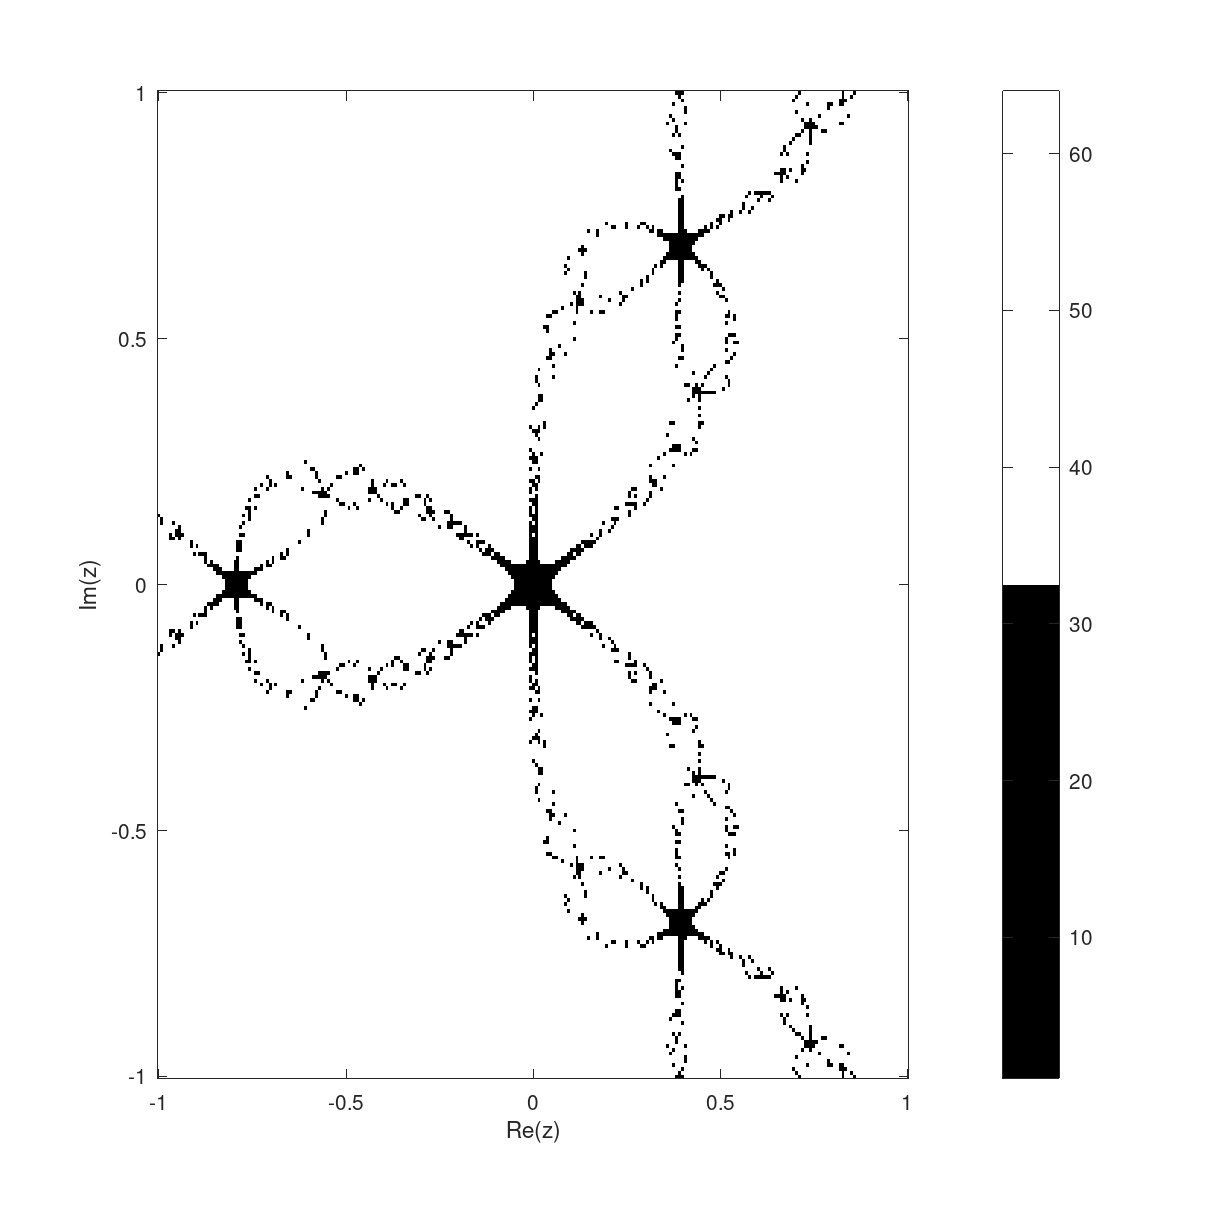
\includegraphics[width=152mm, height=120mm]{images/L2n256maxit16e10-6.png}
    \caption{$L=2$, $n=256$, maxit $=16$, $\epsilon=10^{-6}$}
\end{figure}

\begin{figure}[H]
    \centering
    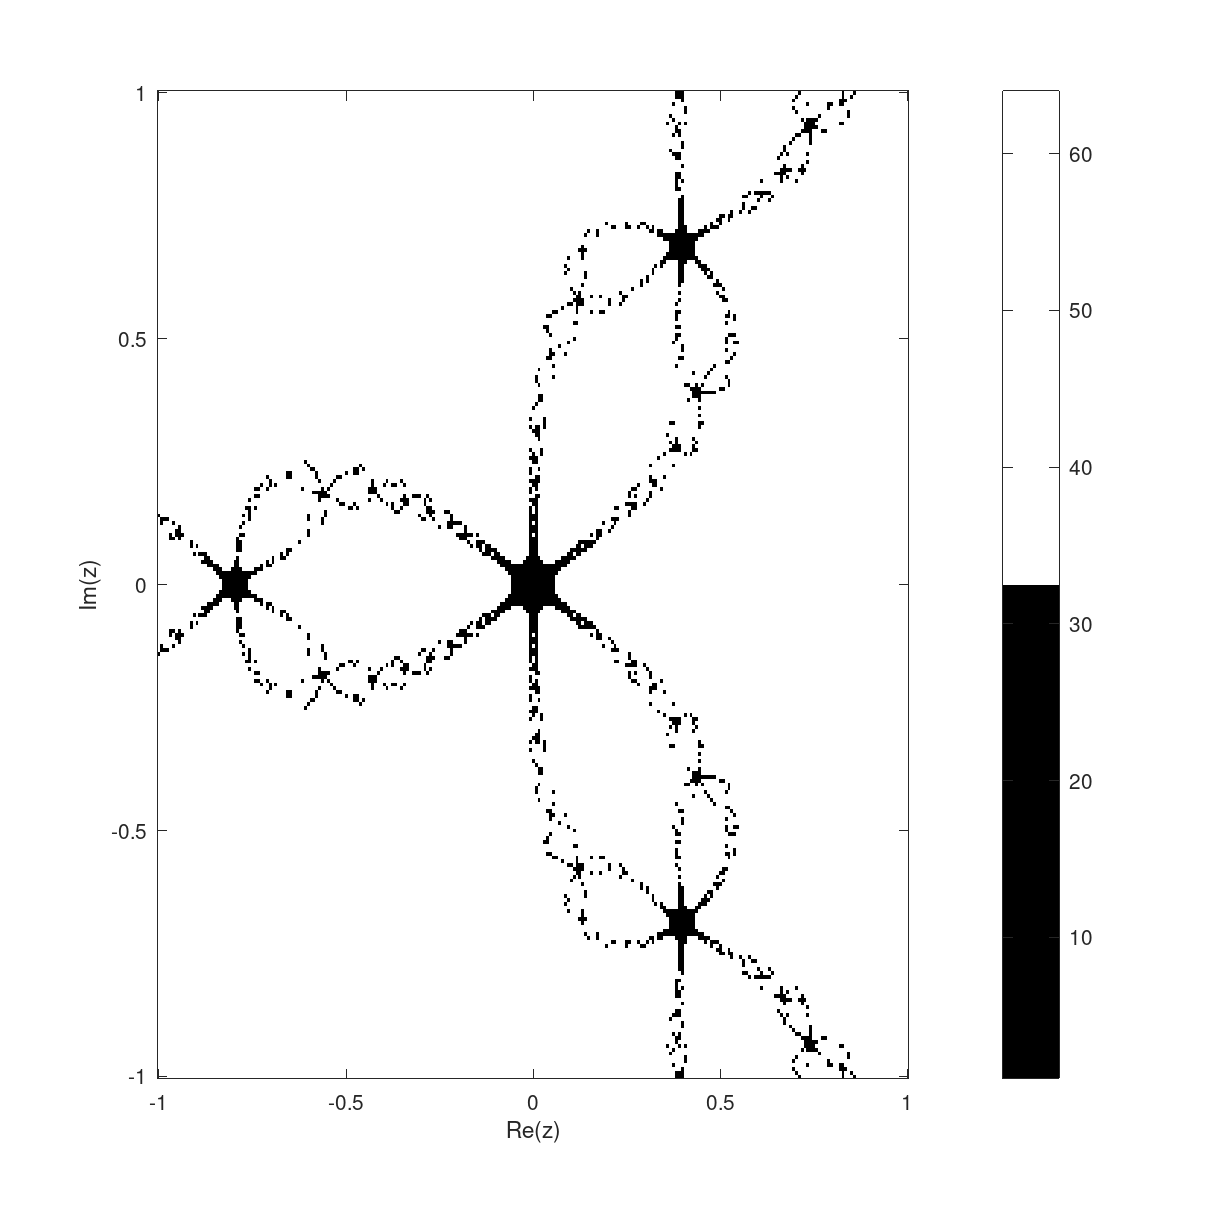
\includegraphics[width=152mm, height=120mm]{images/L2n256maxit16e10-8.png}
    \caption{$L=2$, $n=256$, maxit $=16$, $\epsilon=10^{-8}$}
\end{figure}

\begin{figure}[H]
    \centering
    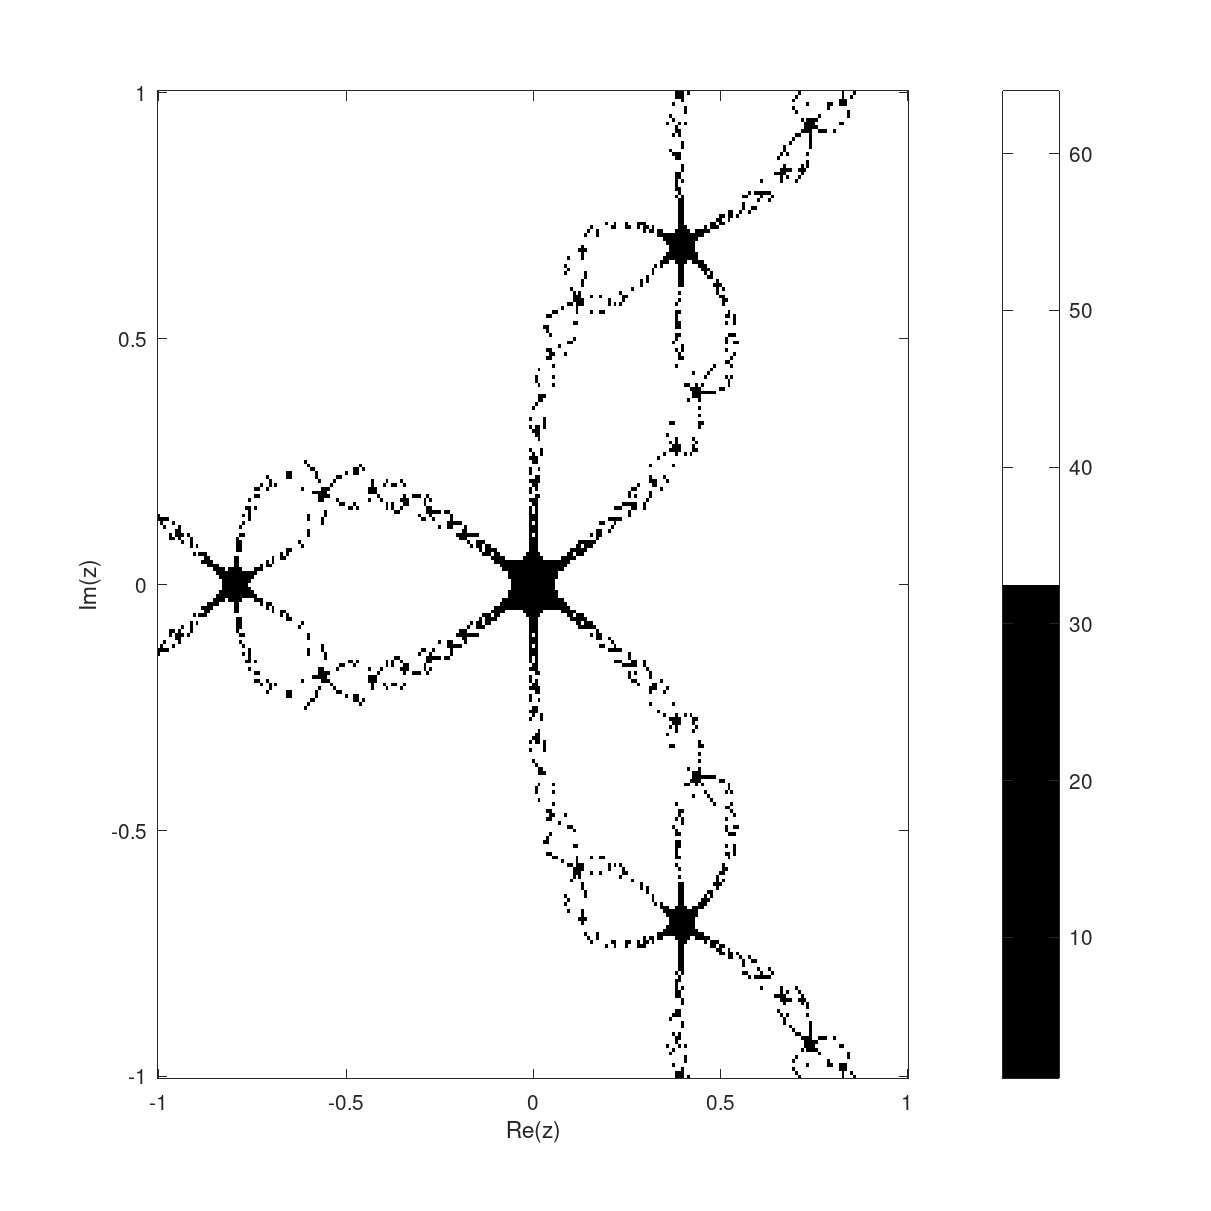
\includegraphics[width=152mm, height=120mm]{images/L2n256maxit16e10-10.png}
    \caption{$L=2$, $n=256$, maxit $=16$, $\epsilon=10^{-10}$}
\end{figure}

\begin{figure}[H]
    \centering
    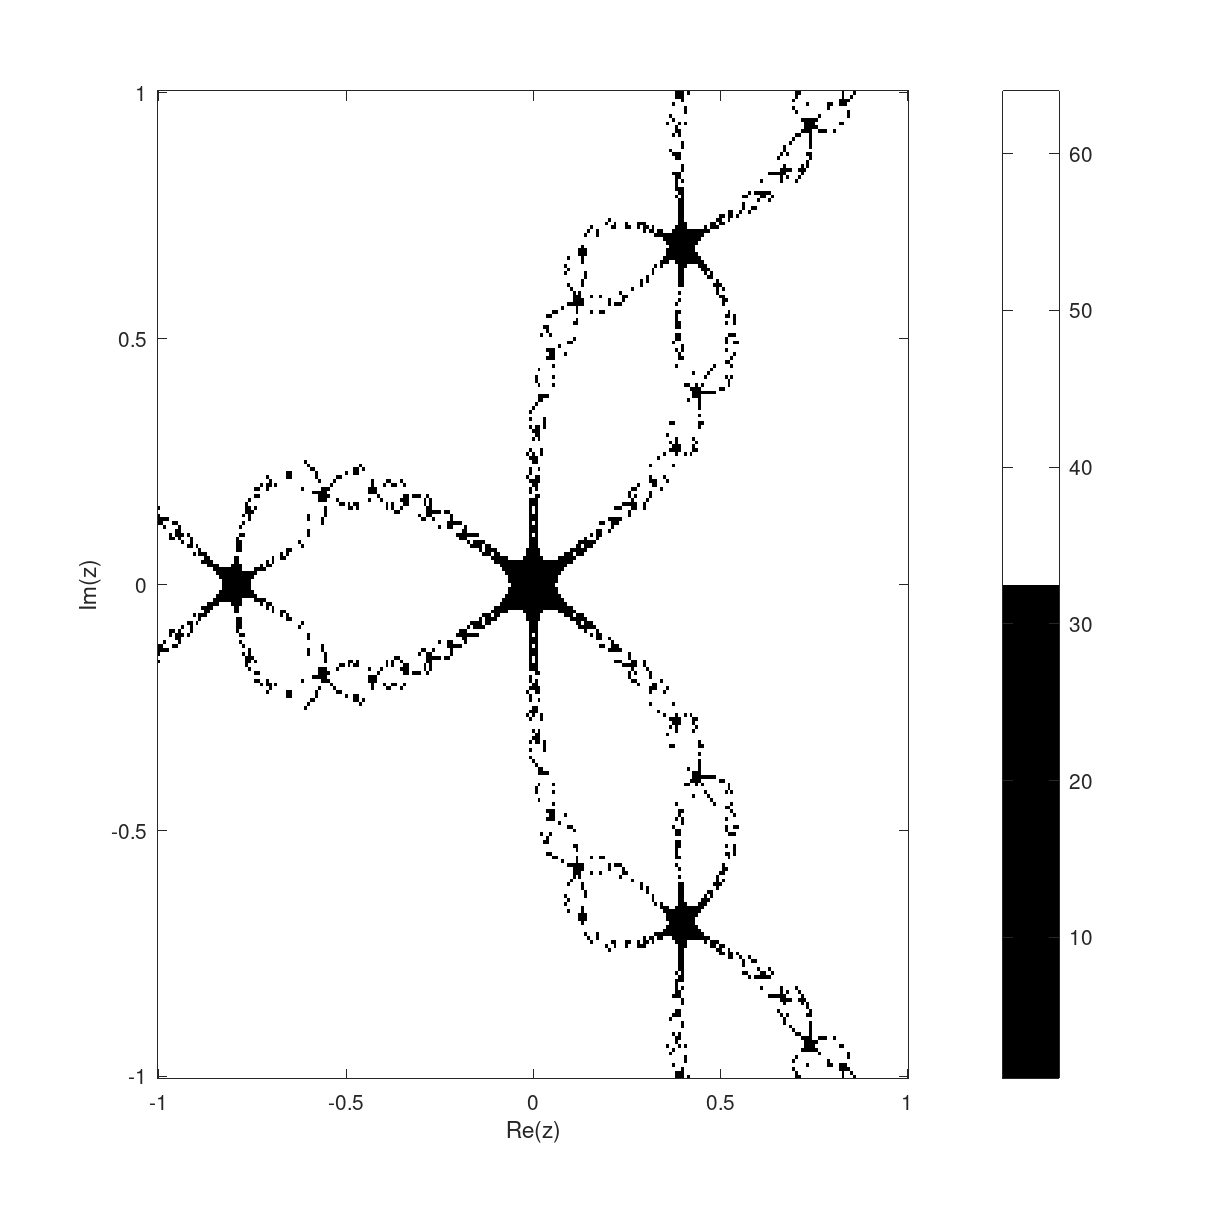
\includegraphics[width=152mm, height=120mm]{images/L2n256maxit16e10-12.png}
    \caption{$L=2$, $n=256$, maxit $=16$, $\epsilon=10^{-12}$}
\end{figure}

\begin{figure}[H]
    \centering
    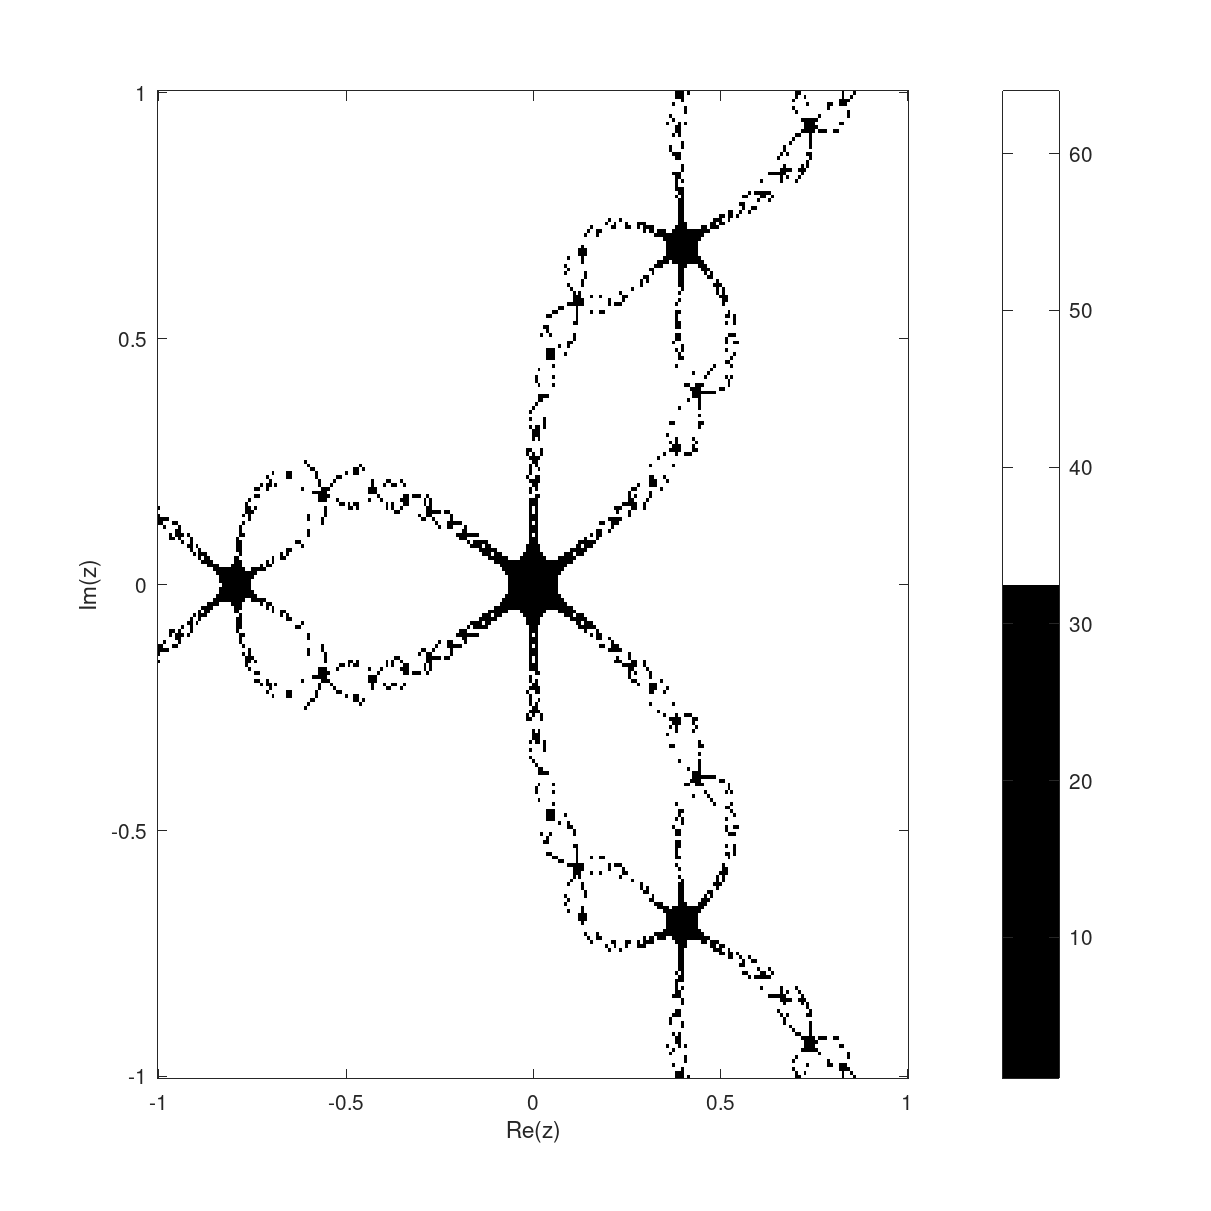
\includegraphics[width=152mm, height=120mm]{images/L2n256maxit16e10-14.png}
    \caption{$L=2$, $n=256$, maxit $=16$, $\epsilon=10^{-14}$}
\end{figure}

\newpage

\textit{ii.} Fije ahora $L=2$, $n=256$, $\epsilon=10^{-10}$ y tome maxit = 8,16,32;

\begin{figure}[H]
    \centering
    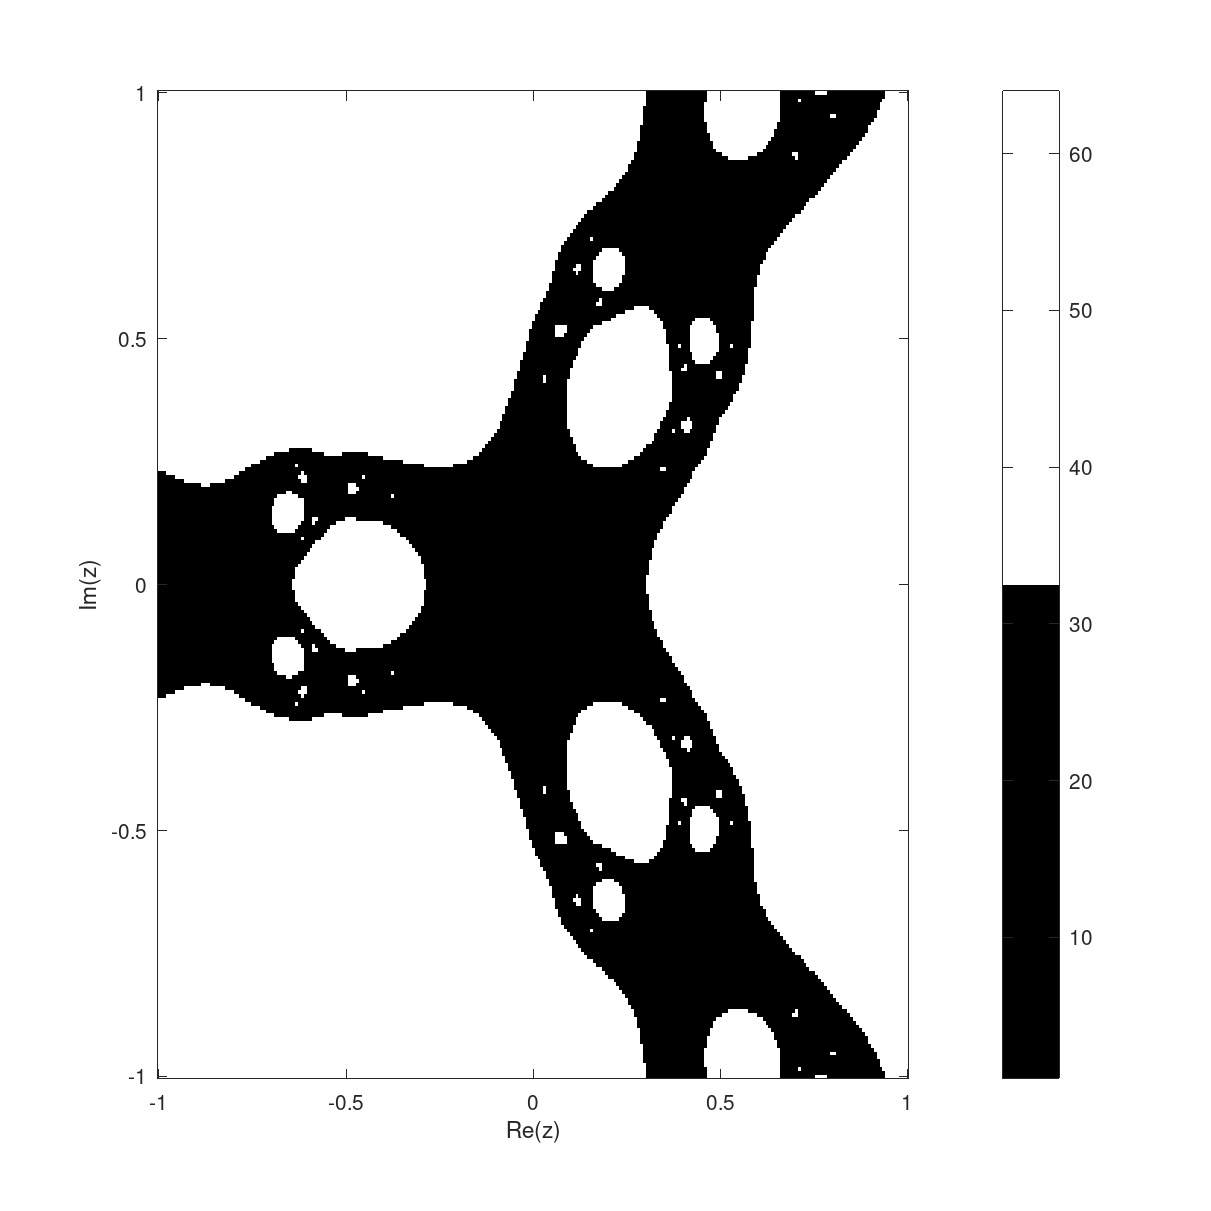
\includegraphics[width=152mm, height=120mm]{images/L2n256maxit8e10-10.png}
    \caption{$L=2$, $n=256$, maxit $=8$, $\epsilon=10^{-10}$}
\end{figure}

\begin{figure}[H]
    \centering
    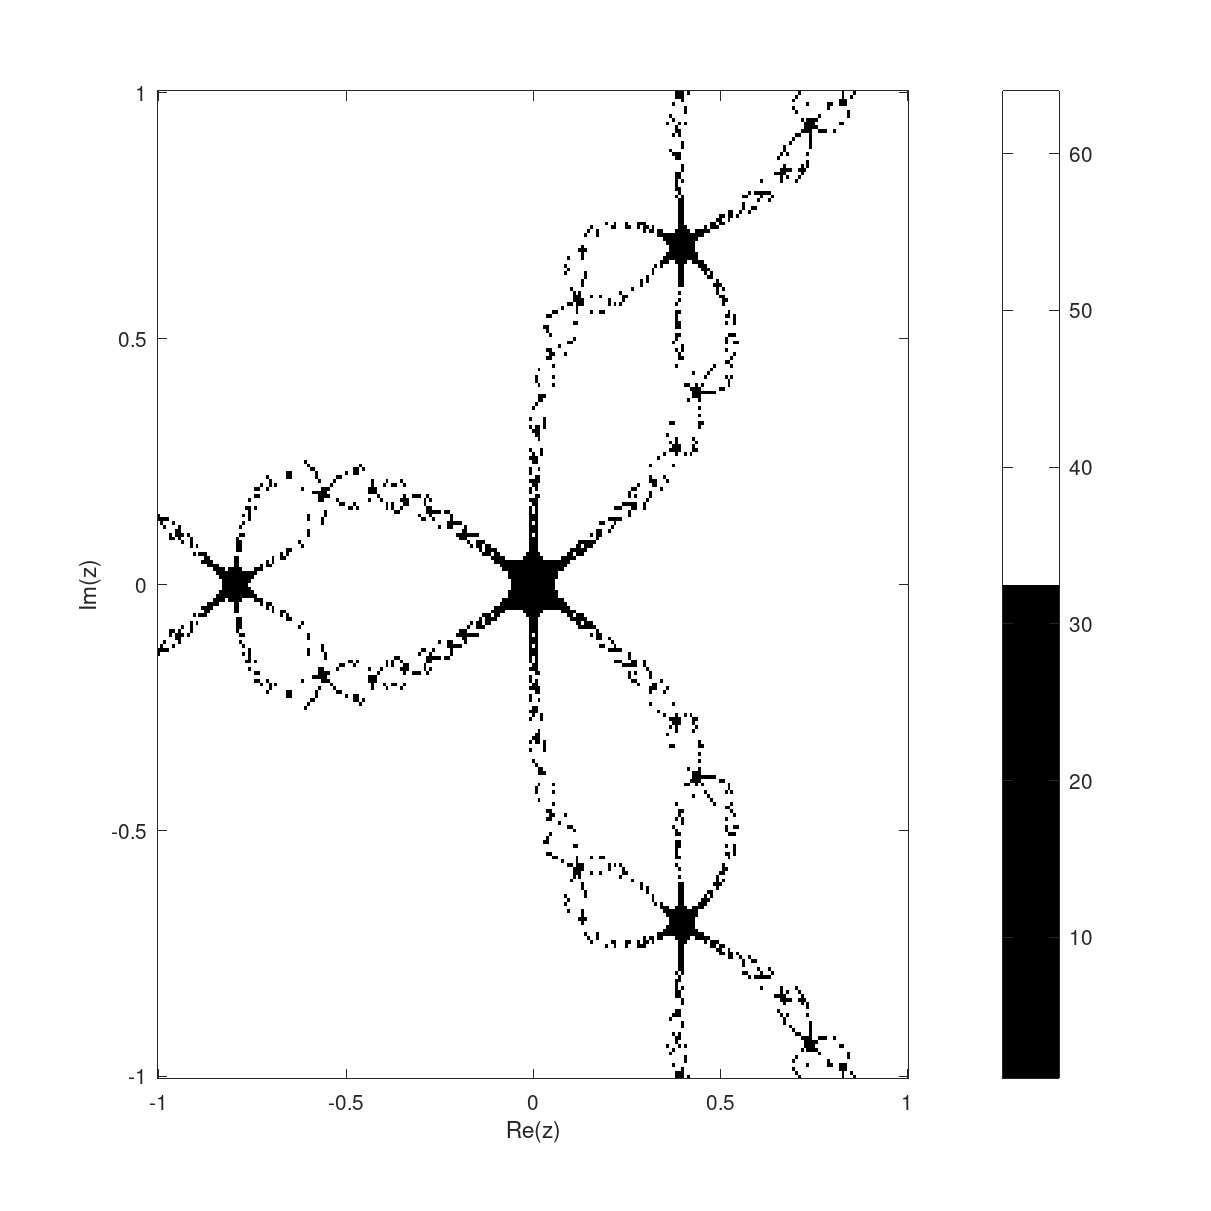
\includegraphics[width=152mm, height=120mm]{images/L2n256maxit16e10-10.png}
    \caption{$L=2$, $n=256$, maxit $=16$, $\epsilon=10^{-10}$}
\end{figure}

\begin{figure}[H]
    \centering
    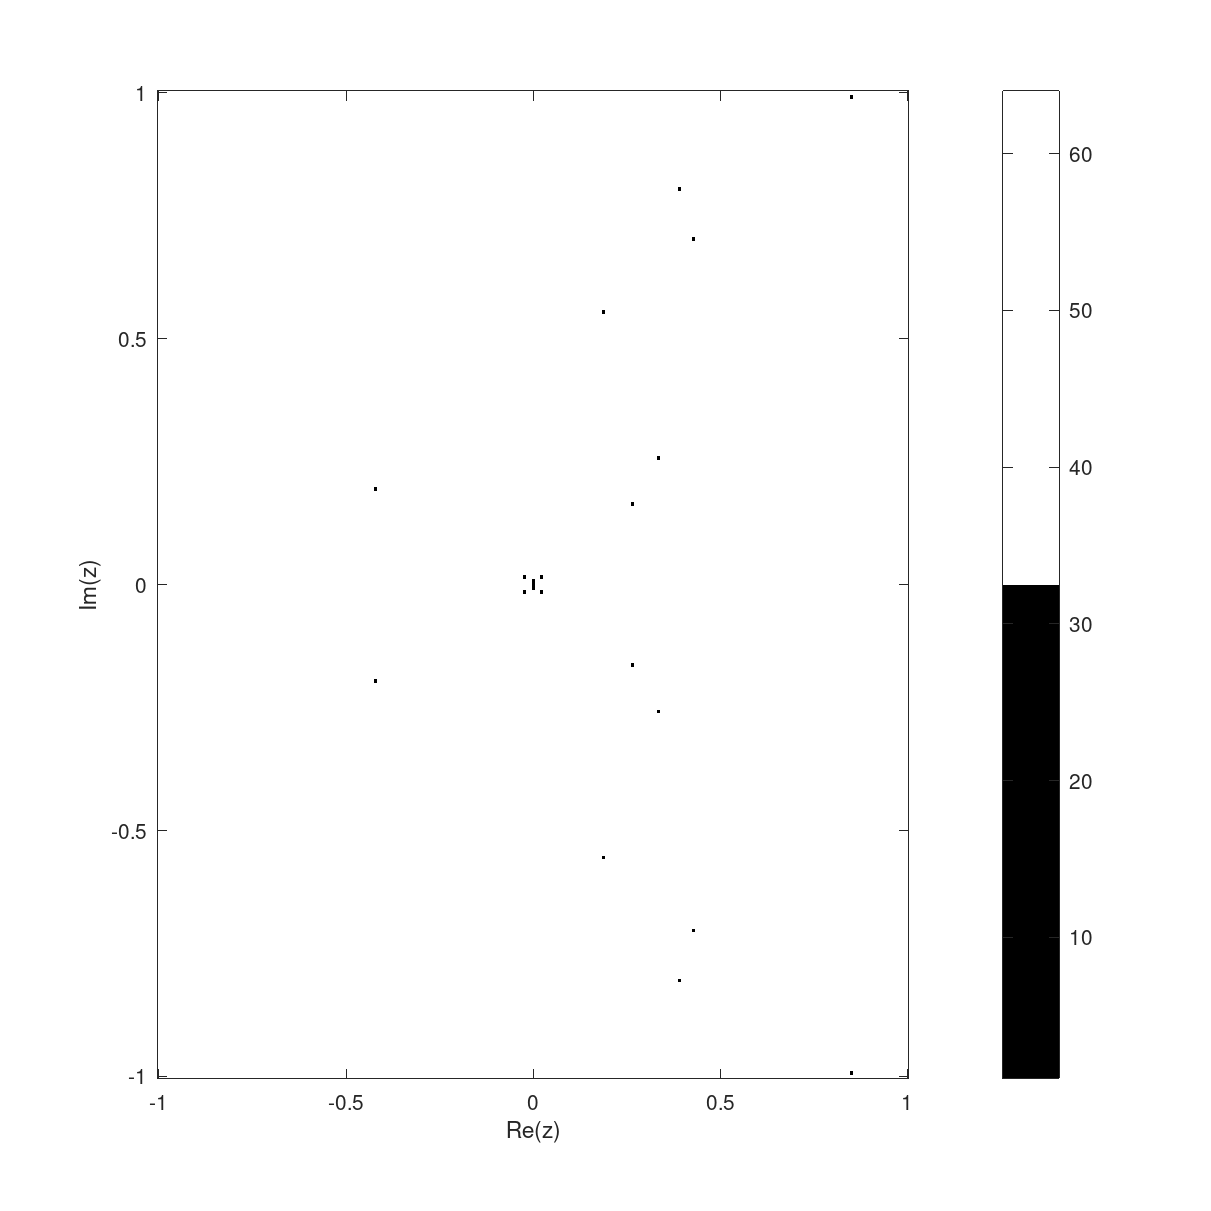
\includegraphics[width=152mm, height=120mm]{images/L2n256maxit32e10-10.png}
    \caption{$L=2$, $n=256$, maxit $=32$, $\epsilon=10^{-10}$}
\end{figure}

\textit{iii.} Fije ahora $L=2$, maxit = 16,  $\epsilon=10^{-10}$ y tome $n=32,64,128,256,512$.

\begin{figure}[H]
    \centering
    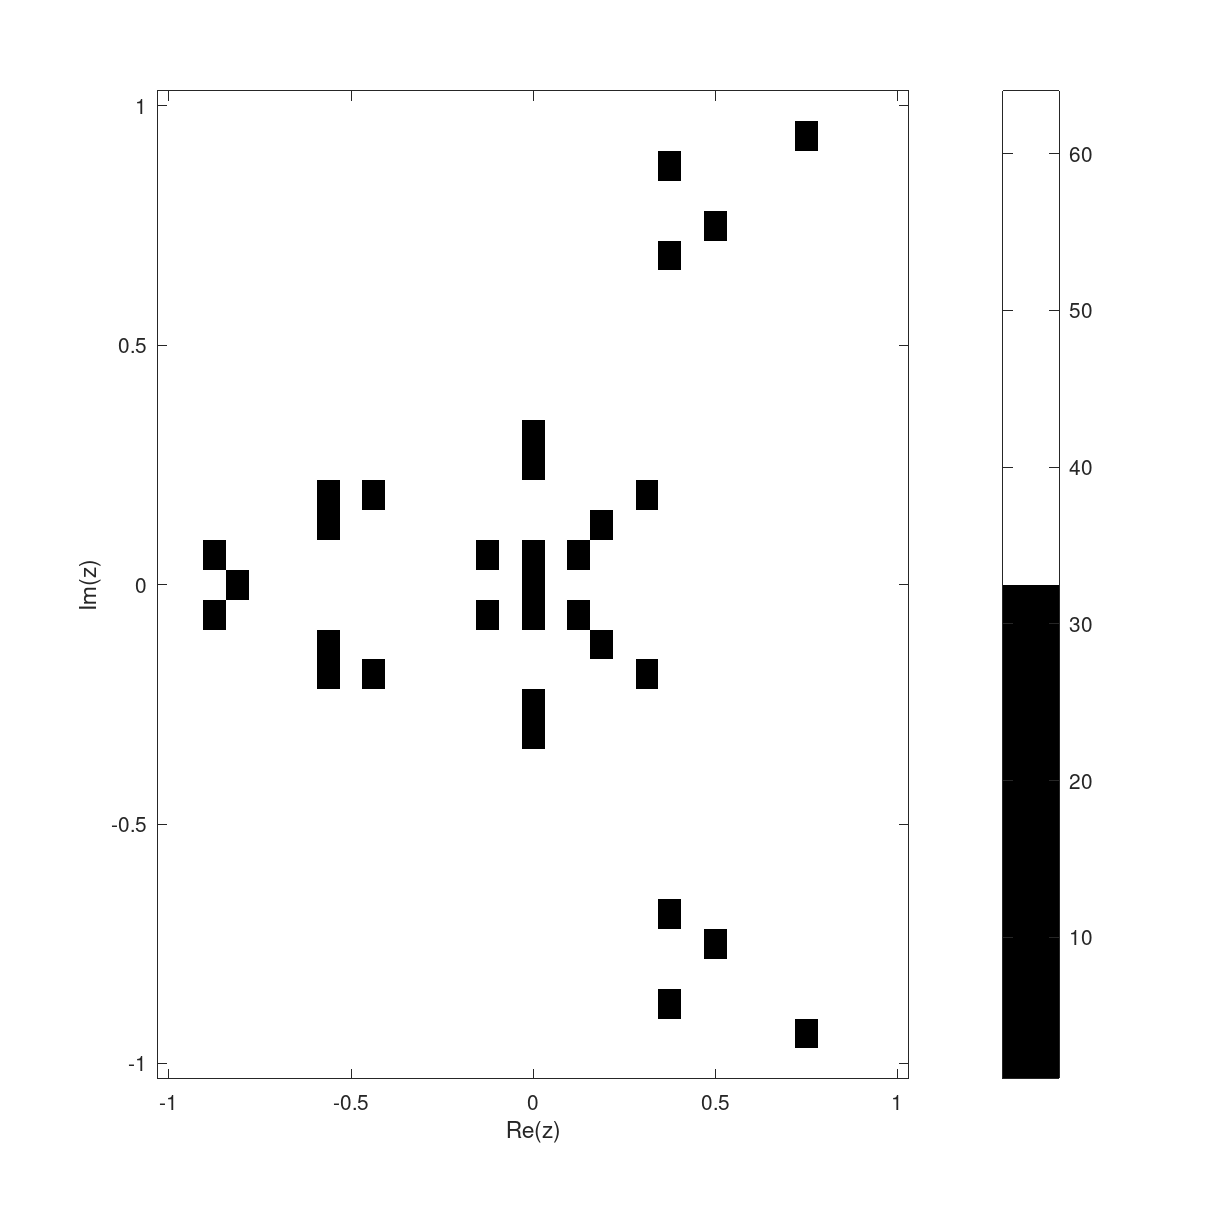
\includegraphics[width=152mm, height=120mm]{images/L2n32maxit16e10-10.png}
    \caption{$L=2$, $n=32$, maxit $=16$, $\epsilon=10^{-10}$}
\end{figure}

\begin{figure}[H]
    \centering
    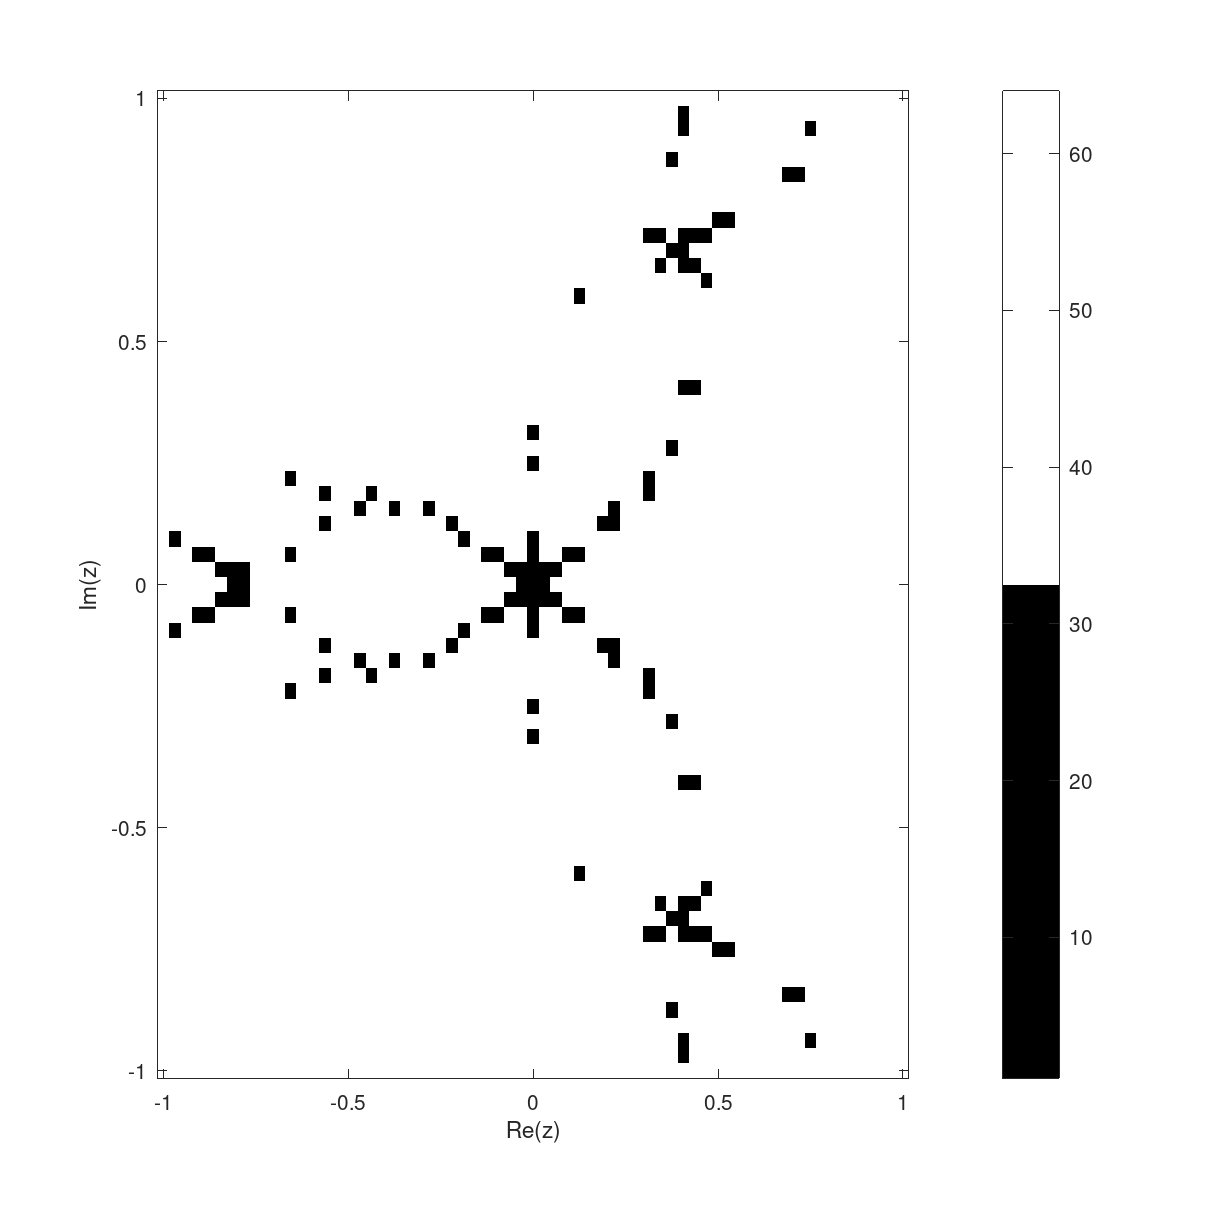
\includegraphics[width=152mm, height=120mm]{images/L2n64maxit16e10-10.png}
    \caption{$L=2$, $n=64$, maxit $=16$, $\epsilon=10^{-10}$}
\end{figure}

\begin{figure}[H]
    \centering
    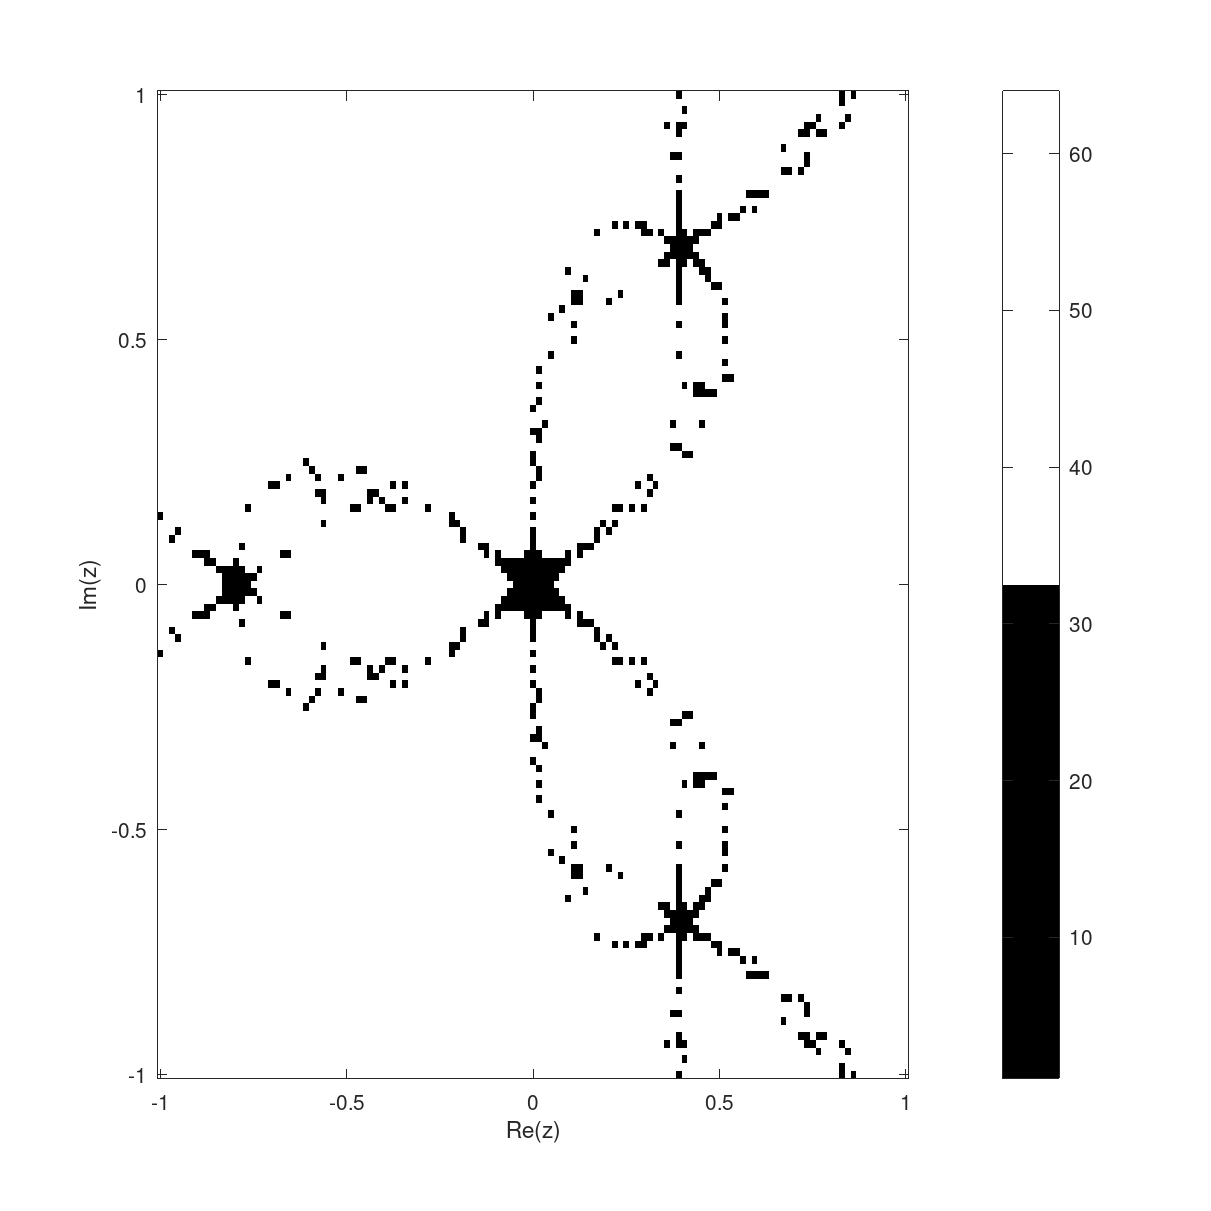
\includegraphics[width=152mm, height=120mm]{images/L2n128maxit16e10-10.png}
    \caption{$L=2$, $n=128$, maxit $=16$, $\epsilon=10^{-10}$}
\end{figure}

\begin{figure}[H]
    \centering
    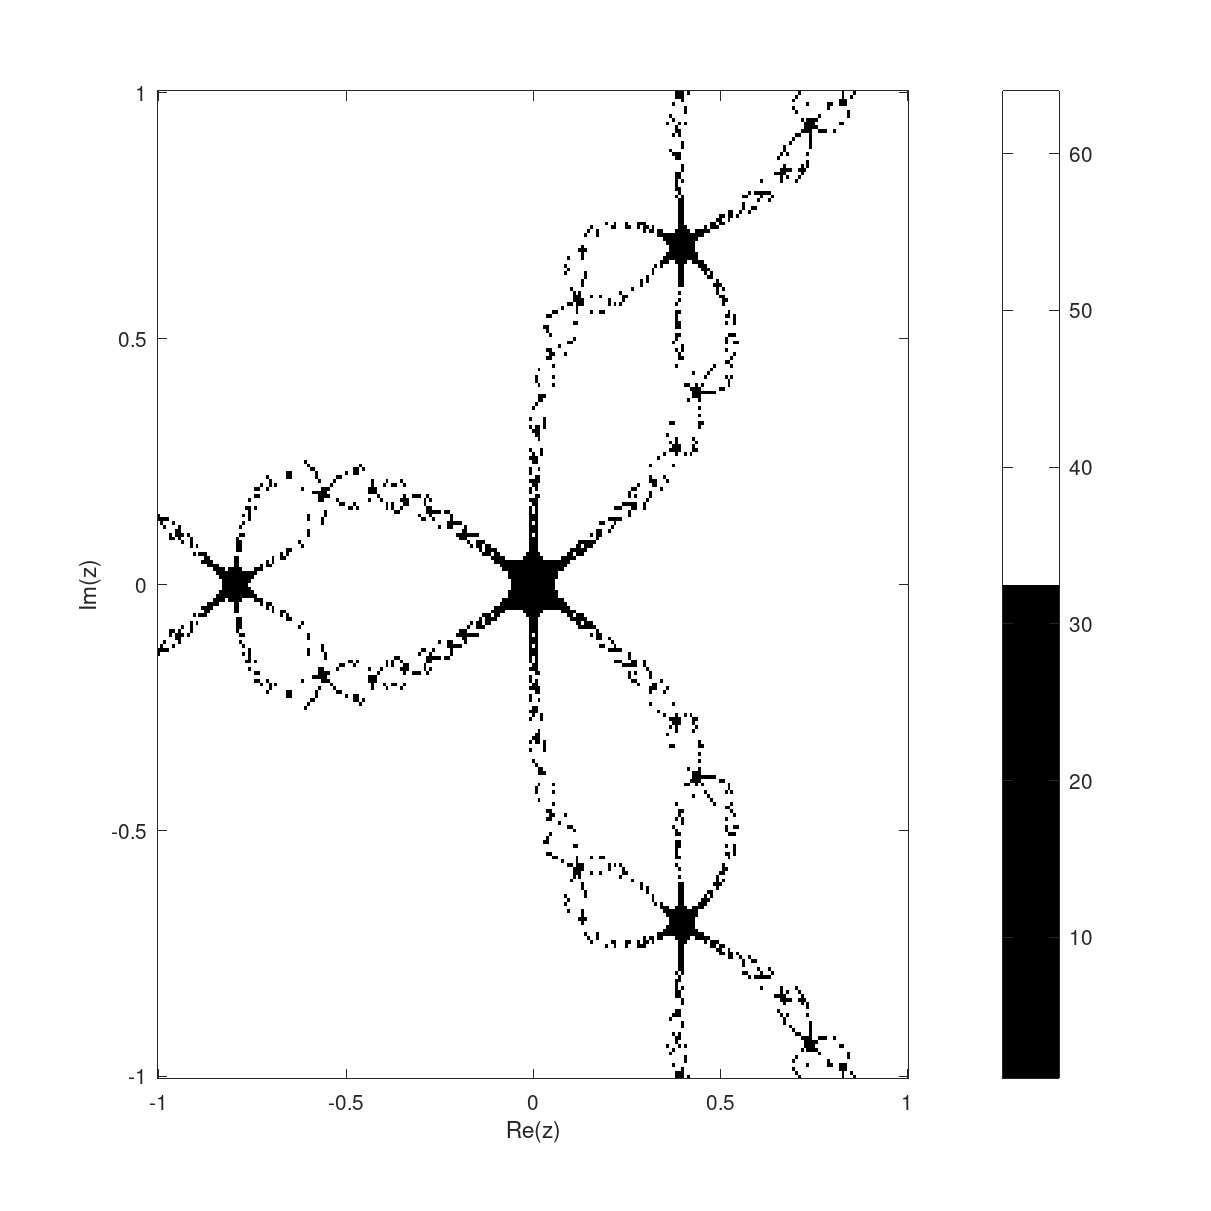
\includegraphics[width=152mm, height=120mm]{images/L2n256maxit16e10-10.png}
    \caption{$L=2$, $n=256$, maxit $=16$, $\epsilon=10^{-10}$}
\end{figure}

\begin{figure}[H]
    \centering
    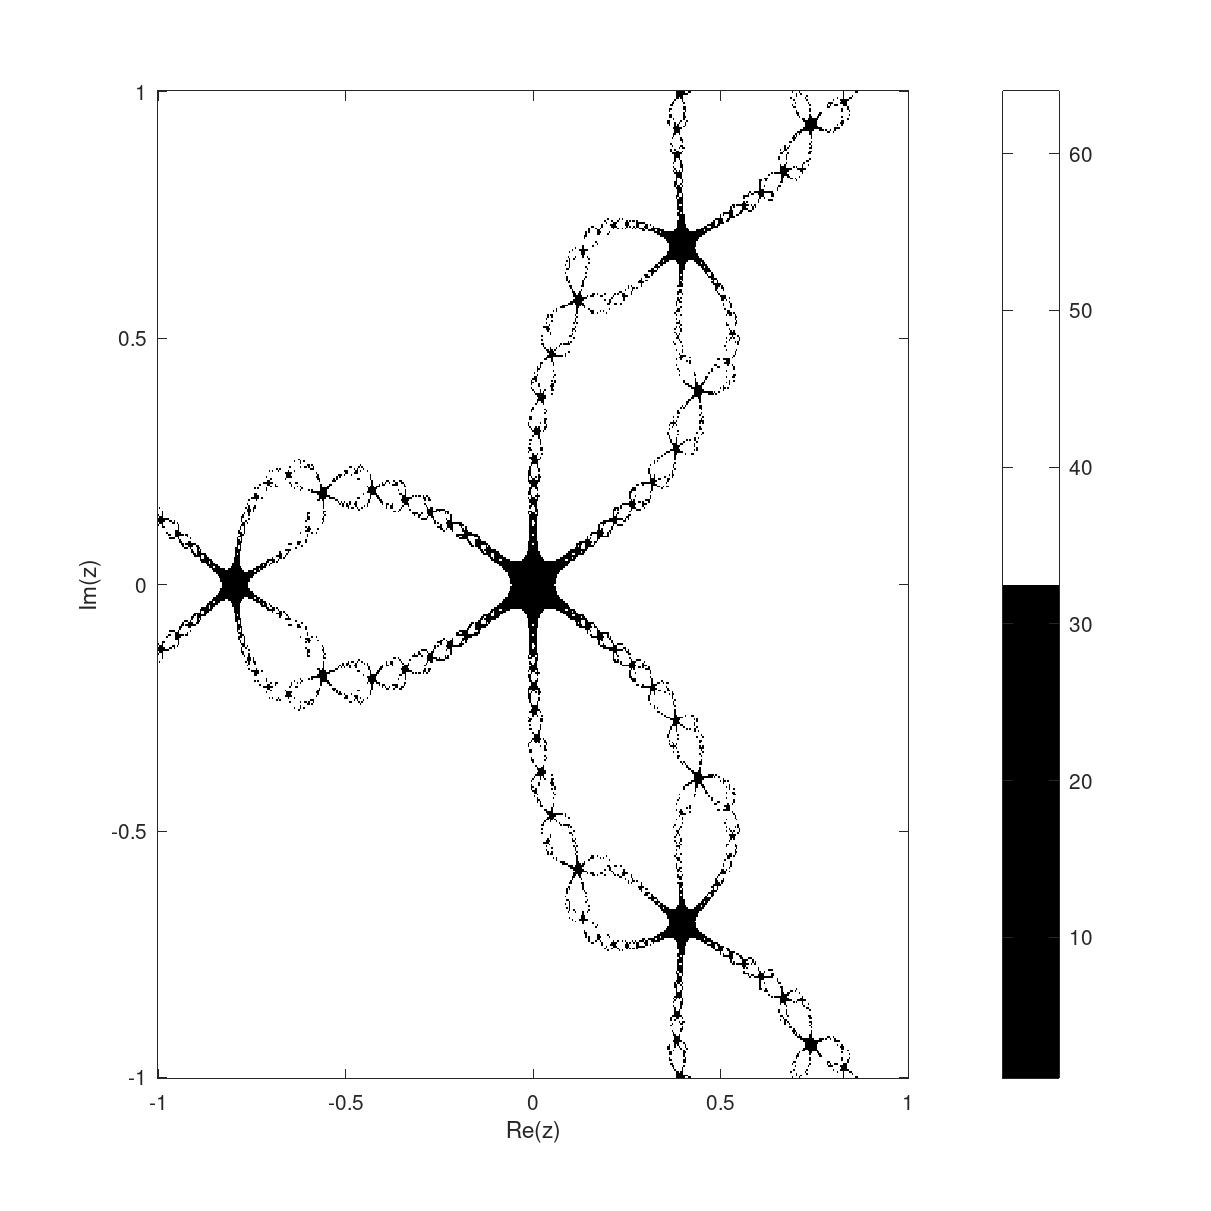
\includegraphics[width=152mm, height=120mm]{images/L2n512maxit16e10-10.png}
    \caption{$L=2$, $n=512$, maxit $=16$, $\epsilon=10^{-10}$}
\end{figure}

\textbf{b.} Repita el inciso a, pero ahora pinte de rojo si el método de Newton llega a la raíz $\alpha_1$, de verde si llega a $\alpha_2$, de azul si llega a $\alpha_3$ y de blanco si no llega a ninguna raíz.

\textit{i} Resuelva con $L=2$,$n=256$, maxit$=16$ fijos y diferentes valores de $\epsilon = 10^{-6},10^{-8},10^{-10},10^{-12}$ y $10^{-14}$

\begin{figure}[H]
    \centering
    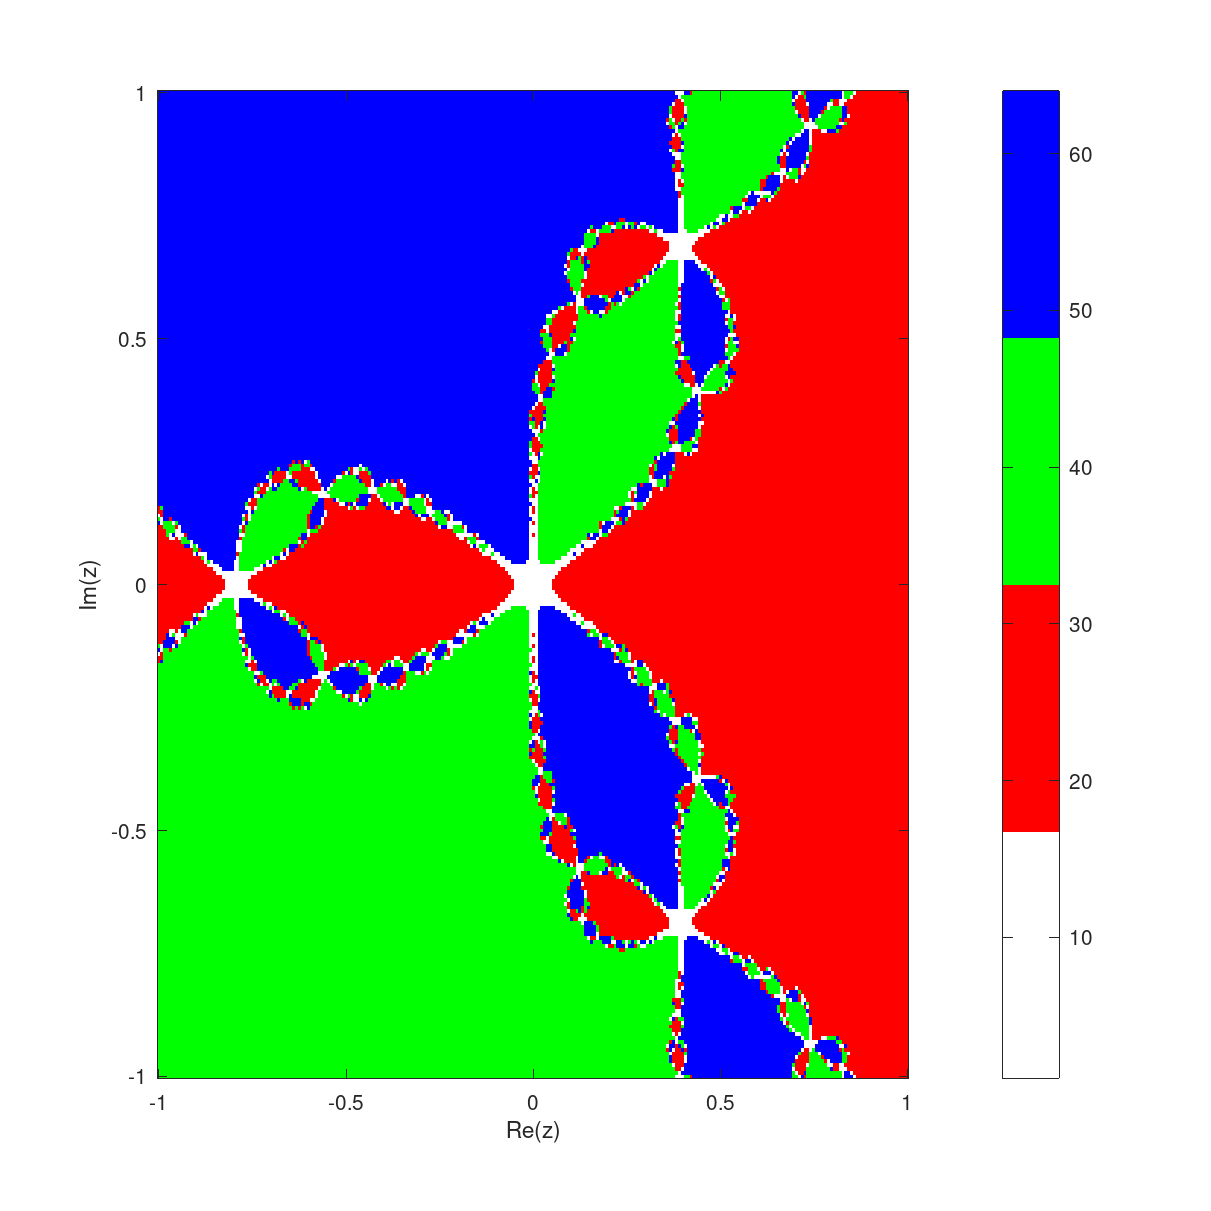
\includegraphics[width=152mm, height=120mm]{images/L2n256maxit16e10-6color.png}
    \caption{$L=2$, $n=256$, maxit $=16$, $\epsilon=10^{-6}$ con colores}
\end{figure}

\begin{figure}[H]
    \centering
    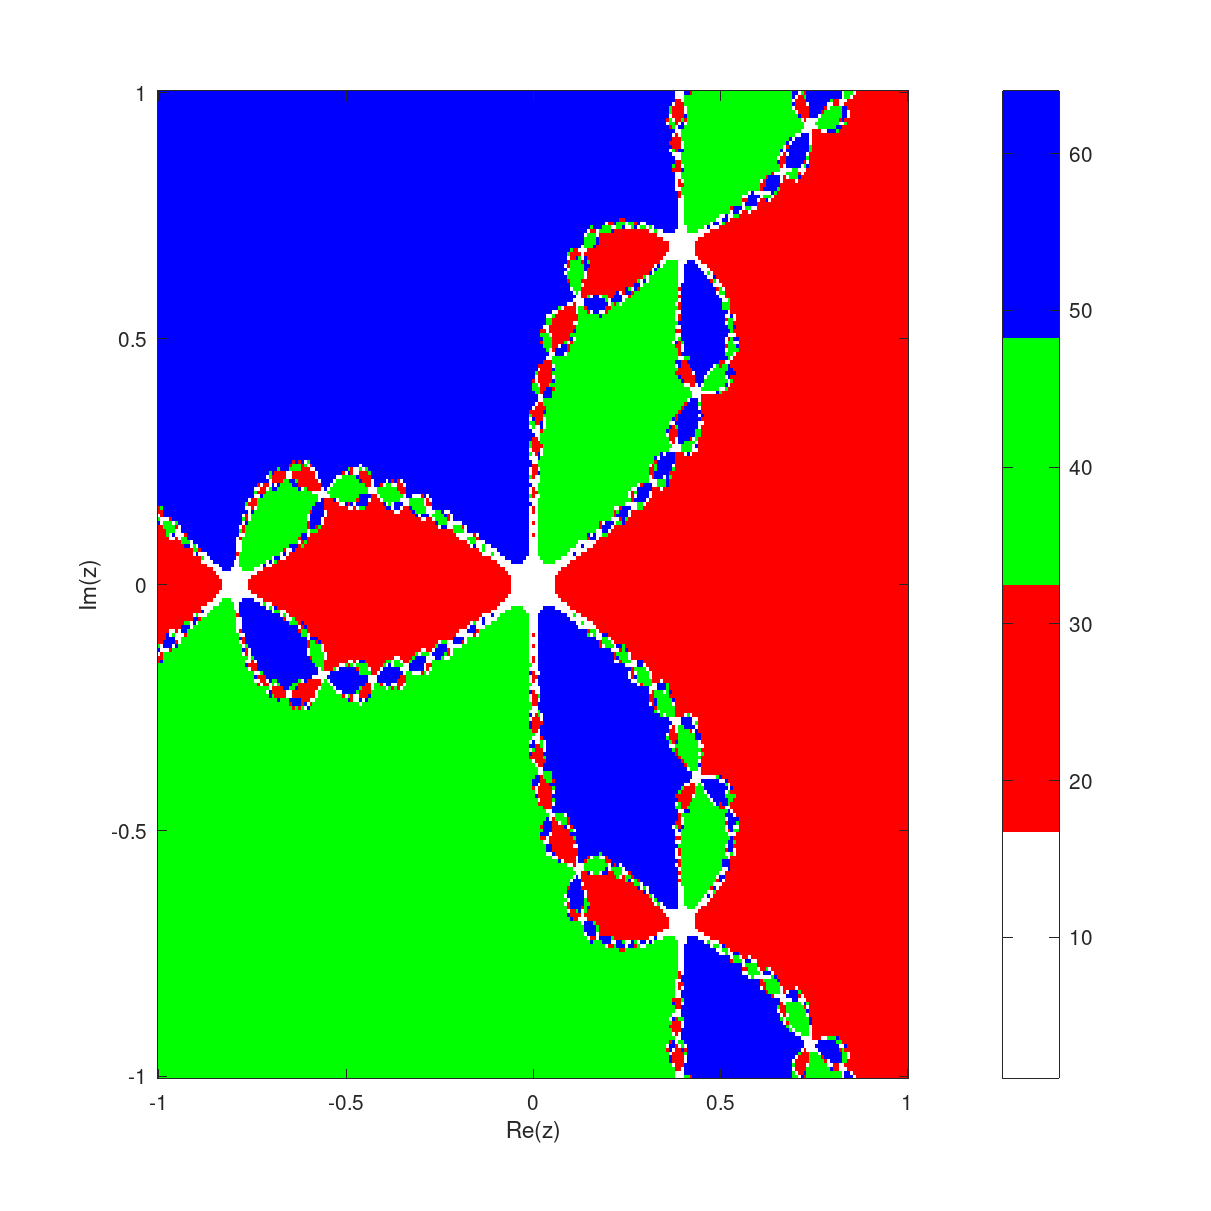
\includegraphics[width=152mm, height=120mm]{images/L2n256maxit16e10-8color.png}
    \caption{$L=2$, $n=256$, maxit $=16$, $\epsilon=10^{-8}$ con colores}
\end{figure}

\begin{figure}[H]
    \centering
    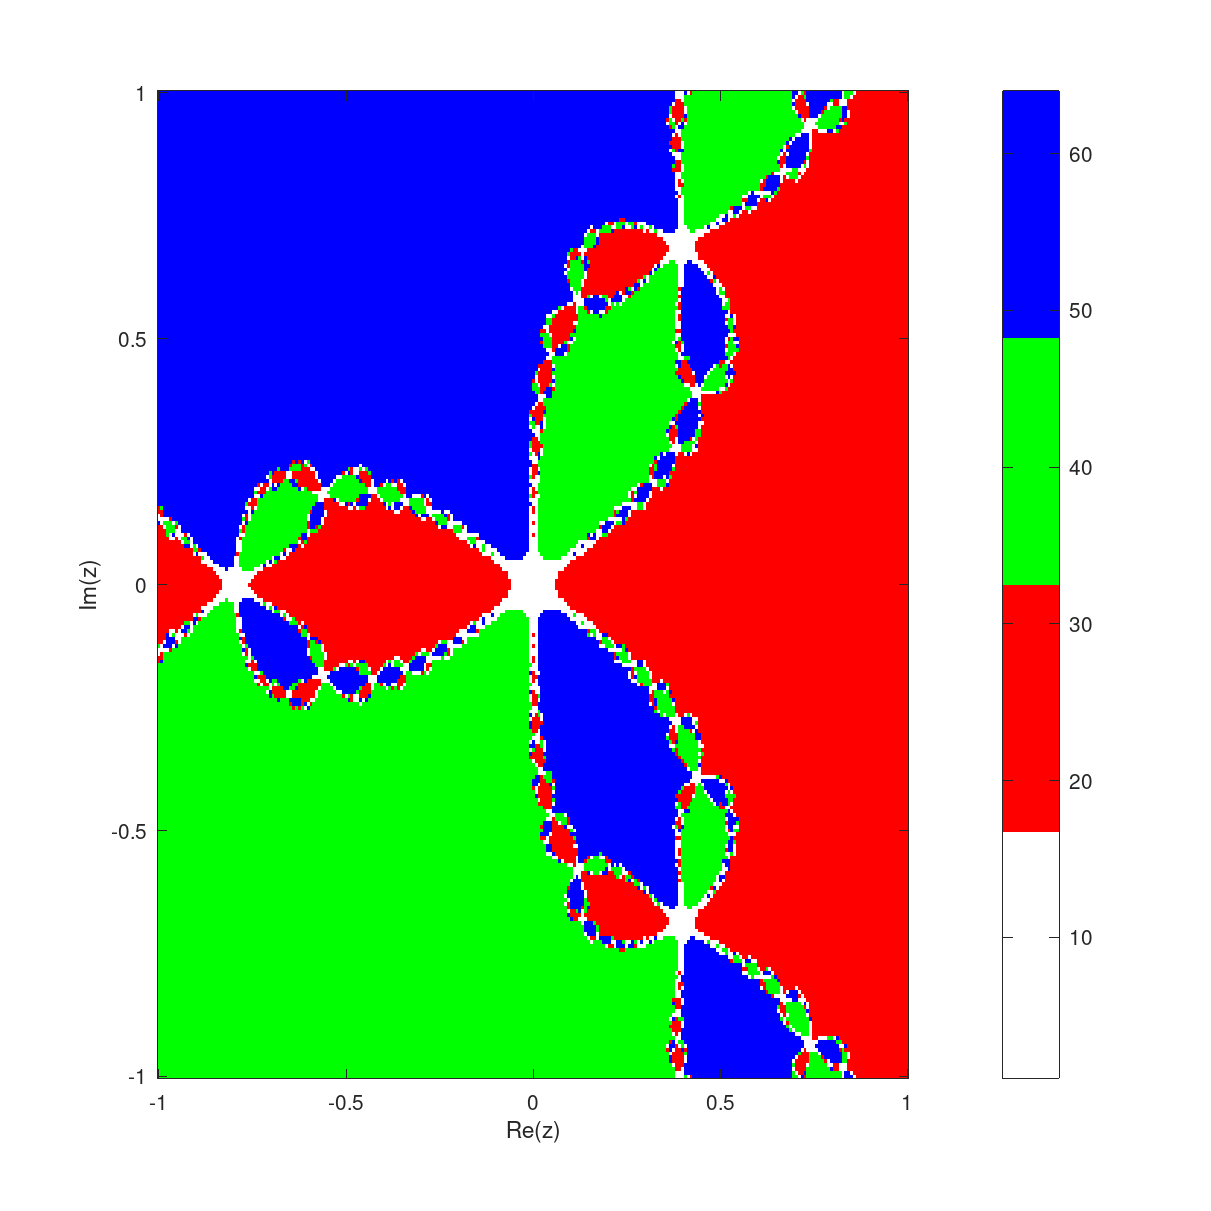
\includegraphics[width=152mm, height=120mm]{images/L2n256maxit16e10-10color.png}
    \caption{$L=2$, $n=256$, maxit $=16$, $\epsilon=10^{-10}$ con colores}
\end{figure}

\begin{figure}[H]
    \centering
    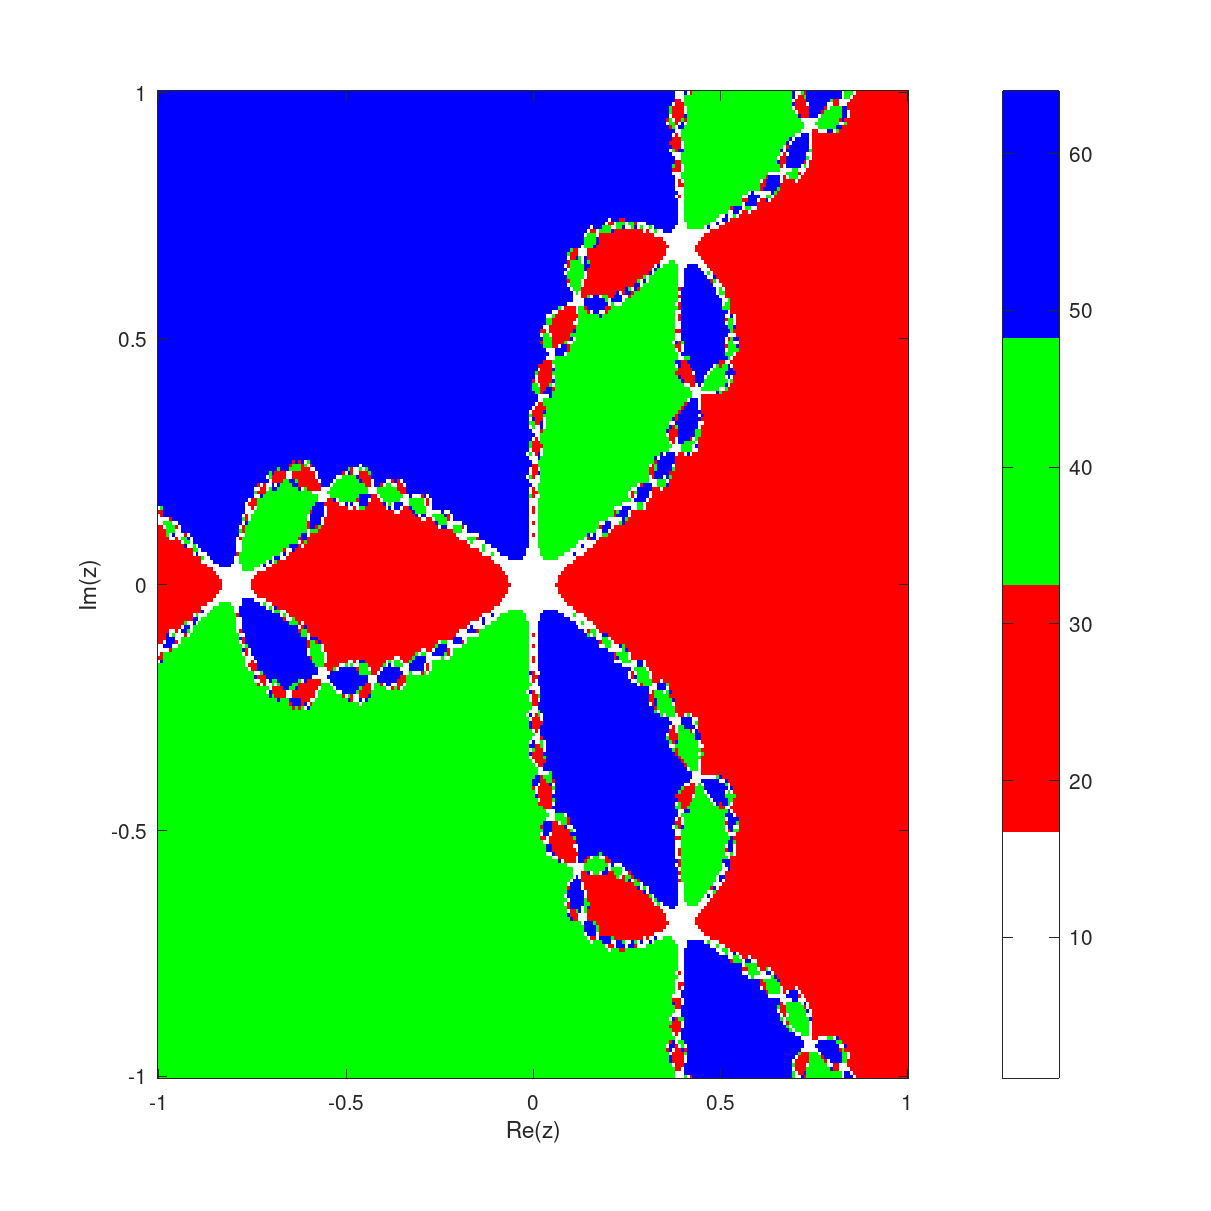
\includegraphics[width=152mm, height=120mm]{images/L2n256maxit16e10-12color.png}
    \caption{$L=2$, $n=256$, maxit $=16$, $\epsilon=10^{-12}$ con colores}
\end{figure}

\begin{figure}[H]
    \centering
    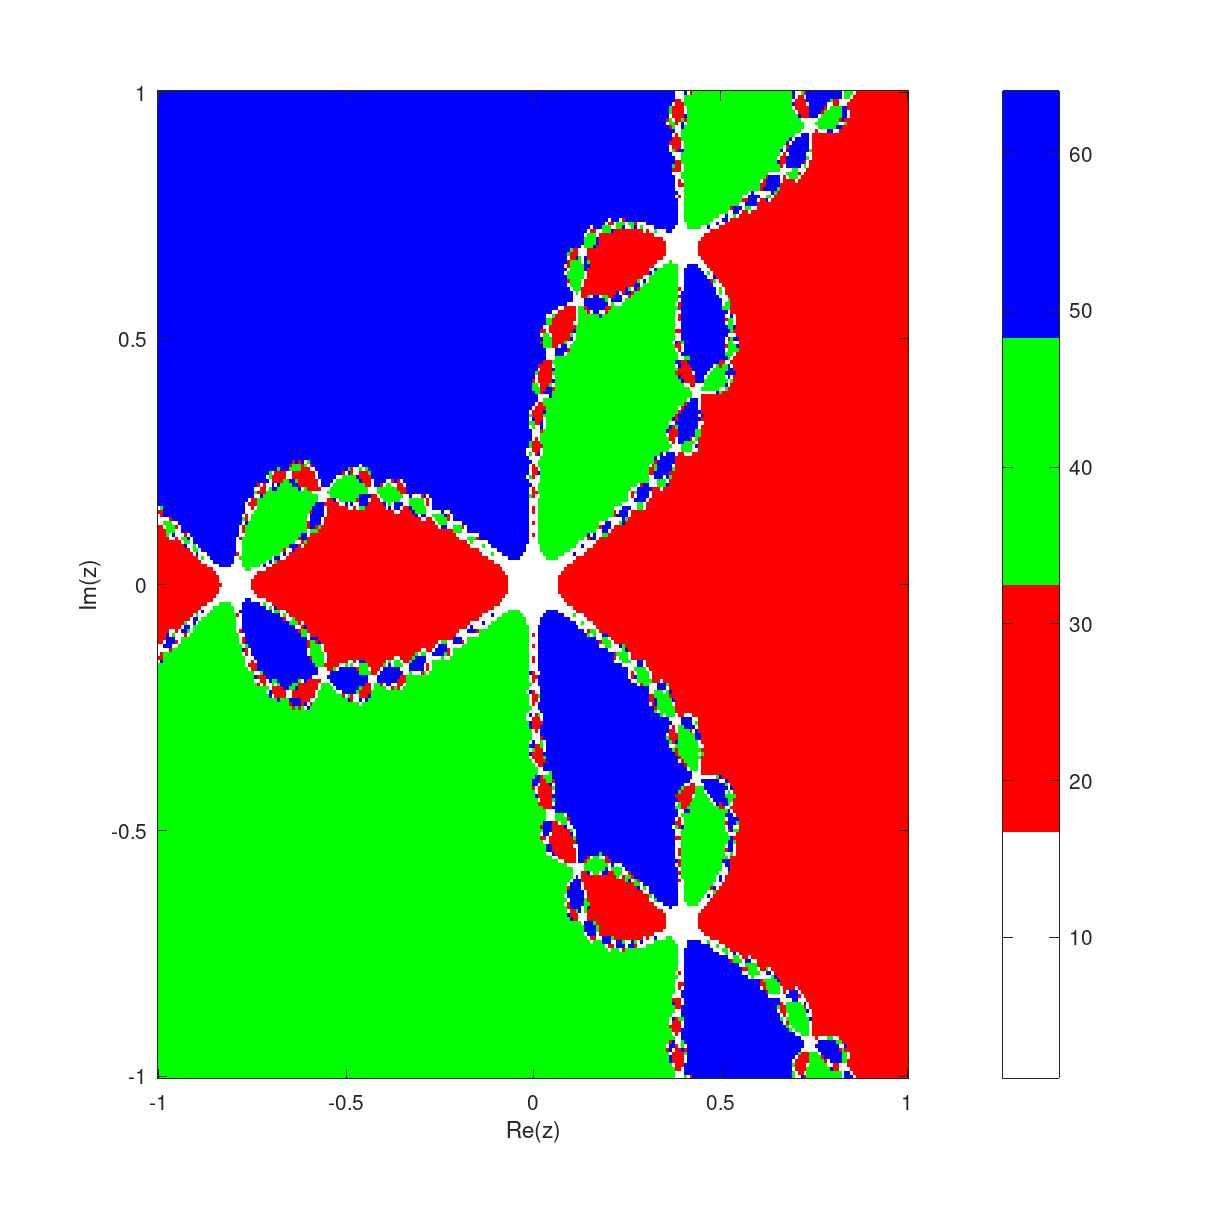
\includegraphics[width=152mm, height=120mm]{images/L2n256maxit16e10-14color.png}
    \caption{$L=2$, $n=256$, maxit $=16$, $\epsilon=10^{-14}$ con colores}
\end{figure}

\newpage

\textit{ii.} Fije ahora $L=2$, $n=256$, $\epsilon=10^{-10}$ y tome maxit = 8,16,32;

\begin{figure}[H]
    \centering
    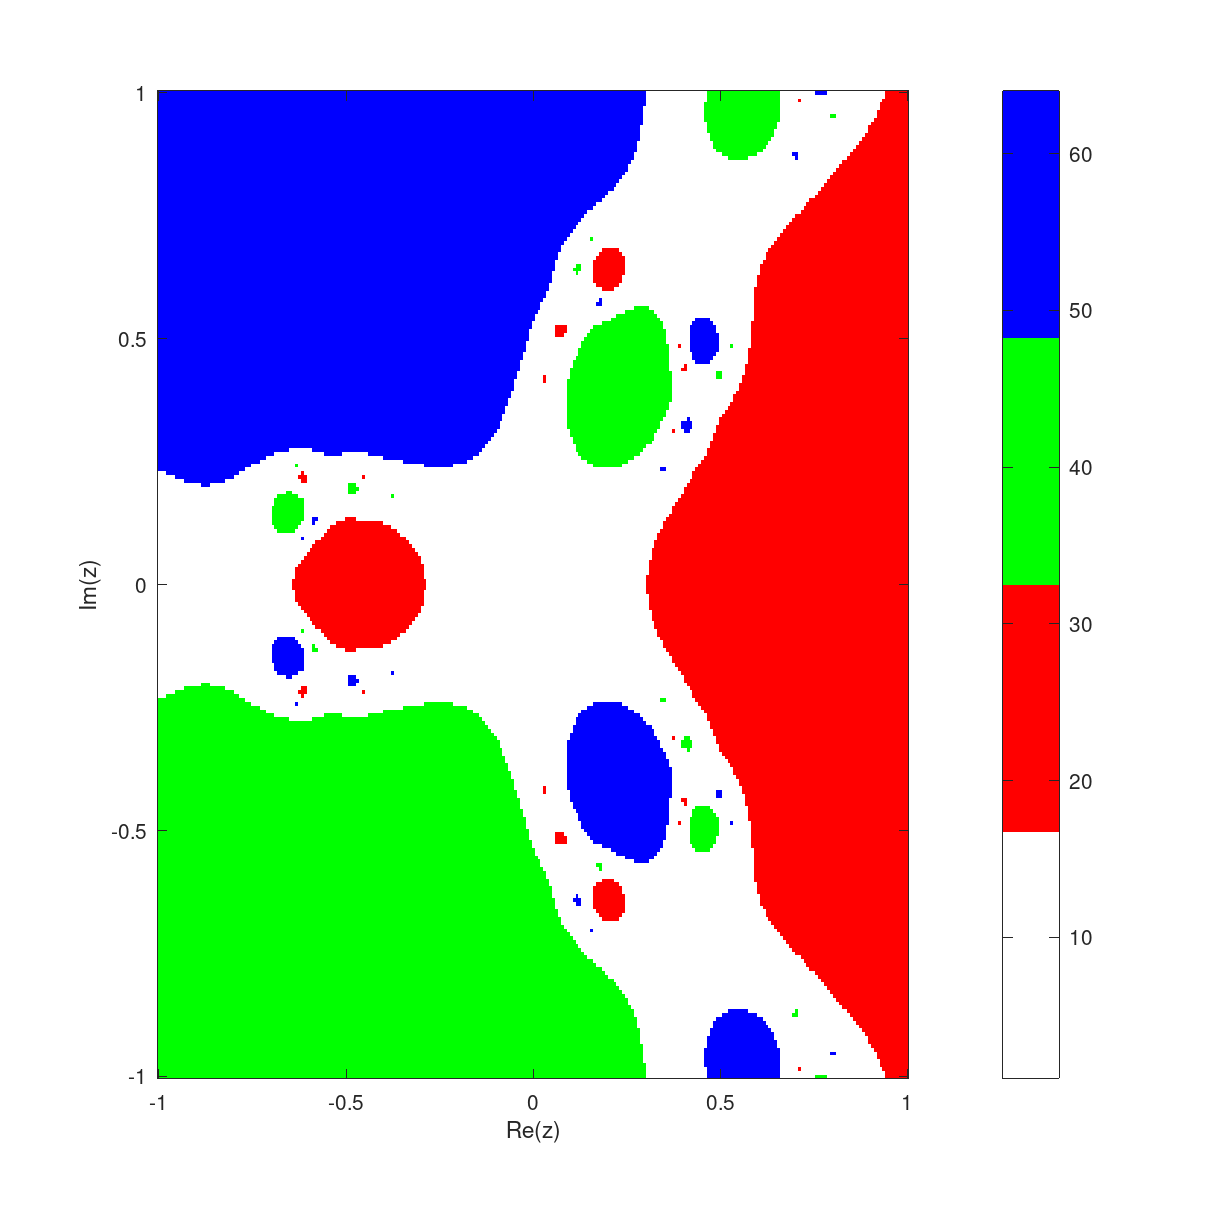
\includegraphics[width=152mm, height=120mm]{images/L2n256maxit8e10-10color.png}
    \caption{$L=2$, $n=256$, maxit $=8$, $\epsilon=10^{-10}$ con colores}
\end{figure}

\begin{figure}[H]
    \centering
    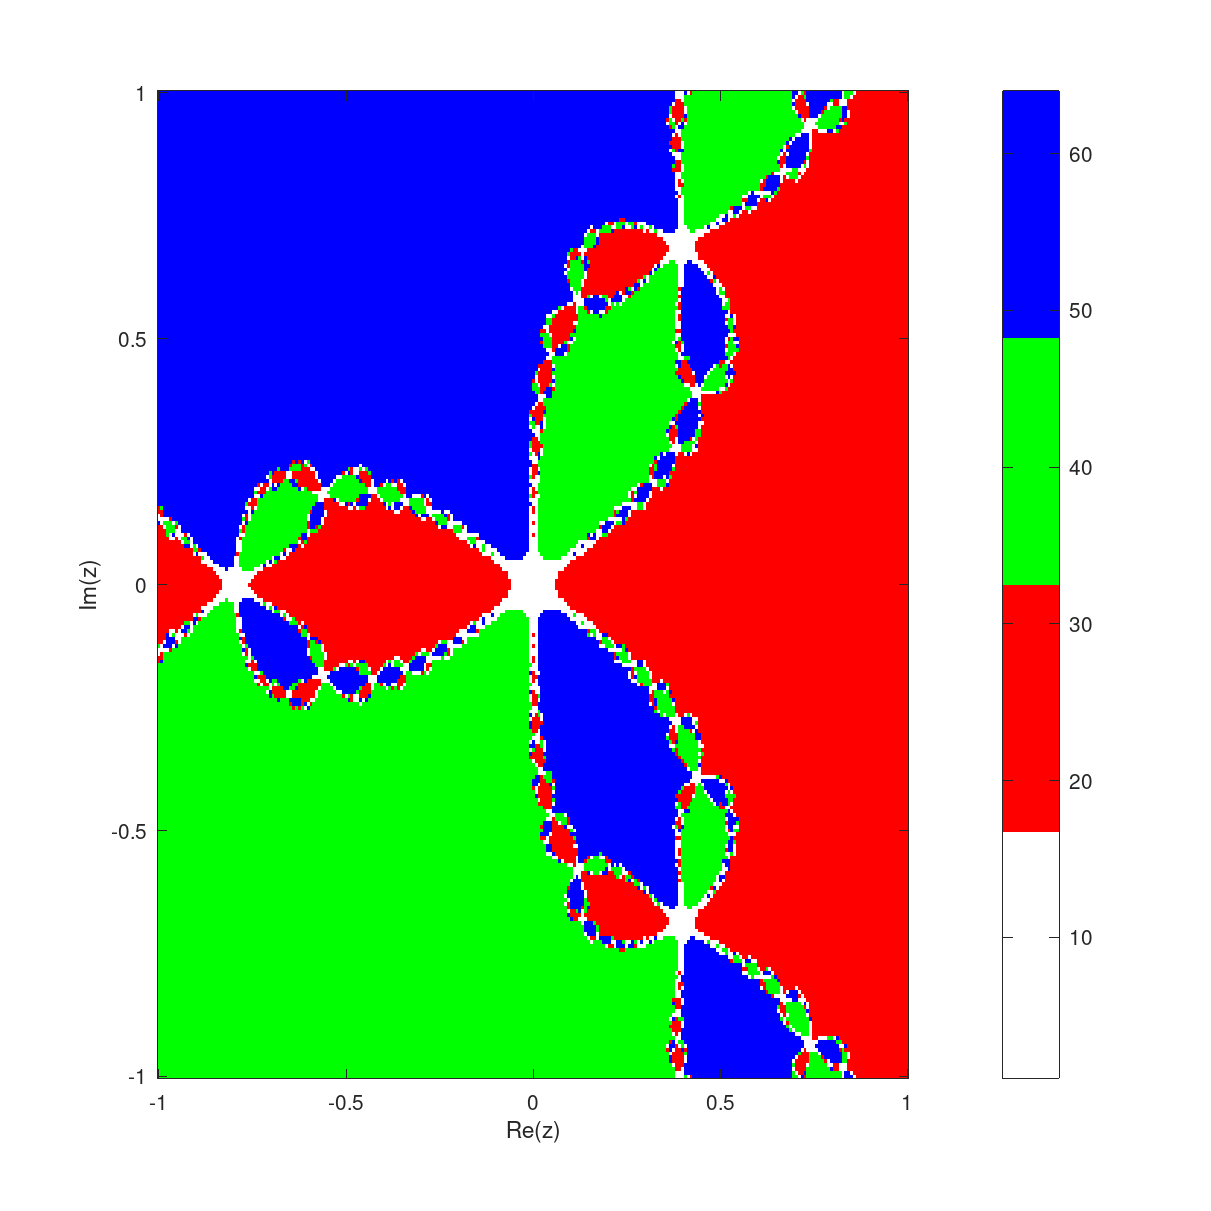
\includegraphics[width=152mm, height=120mm]{images/L2n256maxit16e10-10color.png}
    \caption{$L=2$, $n=256$, maxit $=16$, $\epsilon=10^{-10}$ con colores}
\end{figure}

\begin{figure}[H]
    \centering
    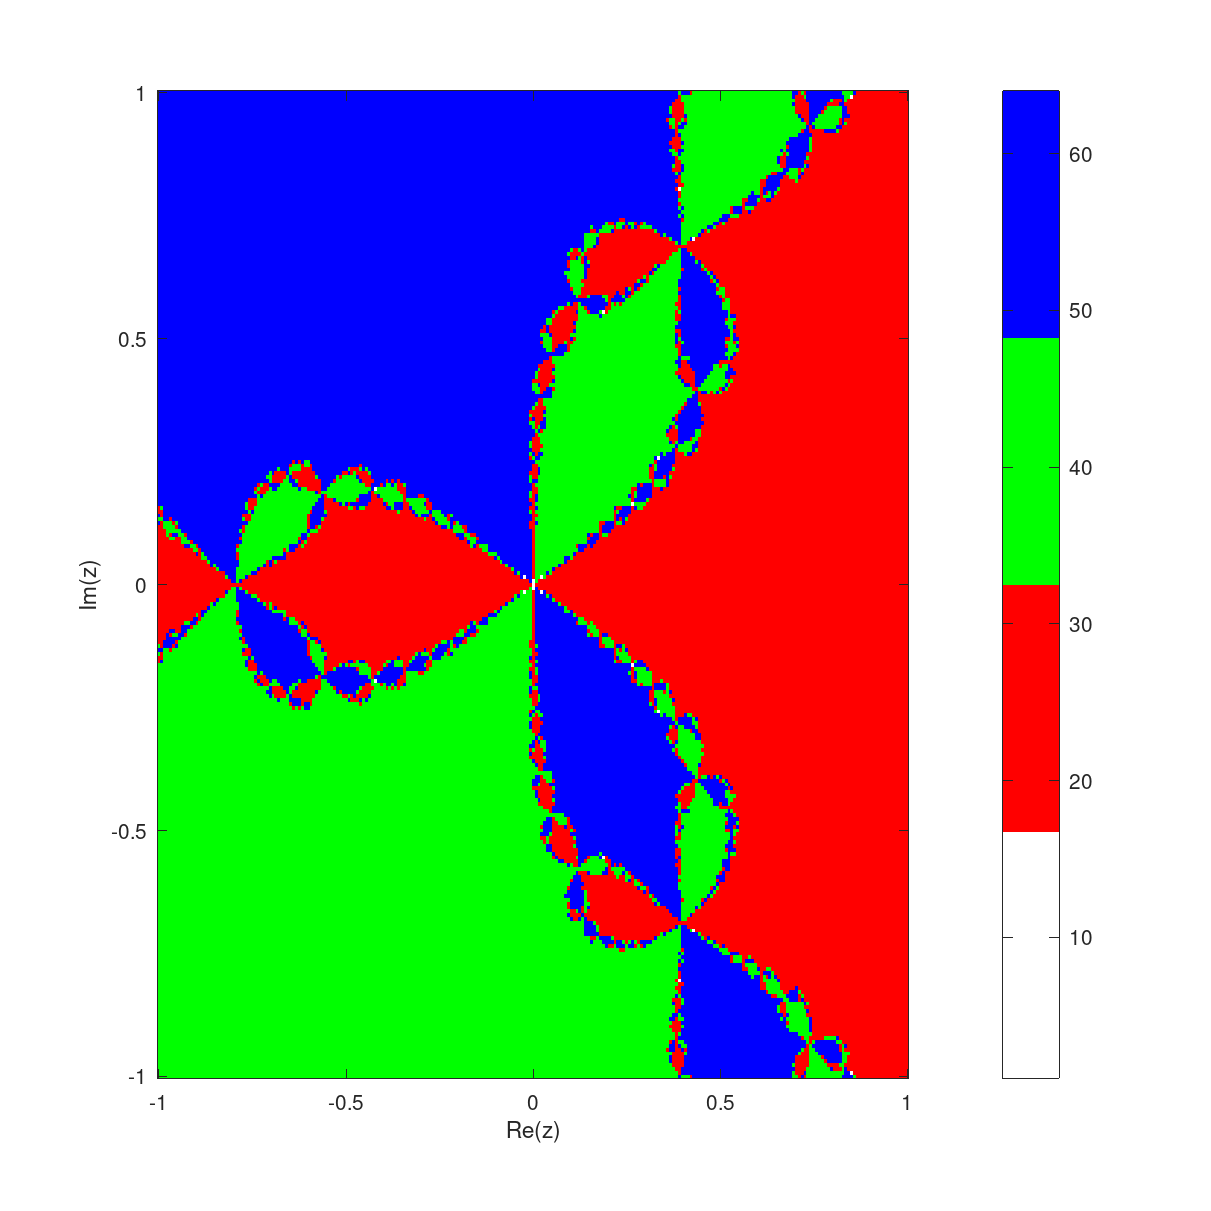
\includegraphics[width=152mm, height=120mm]{images/L2n256maxit32e10-10color.png}
    \caption{$L=2$, $n=256$, maxit $=32$, $\epsilon=10^{-10}$ con colores}
\end{figure}

\textit{iii.} Fije ahora $L=2$, maxit = 16,  $\epsilon=10^{-10}$ y tome $n=32,64,128,256,512$.

\begin{figure}[H]
    \centering
    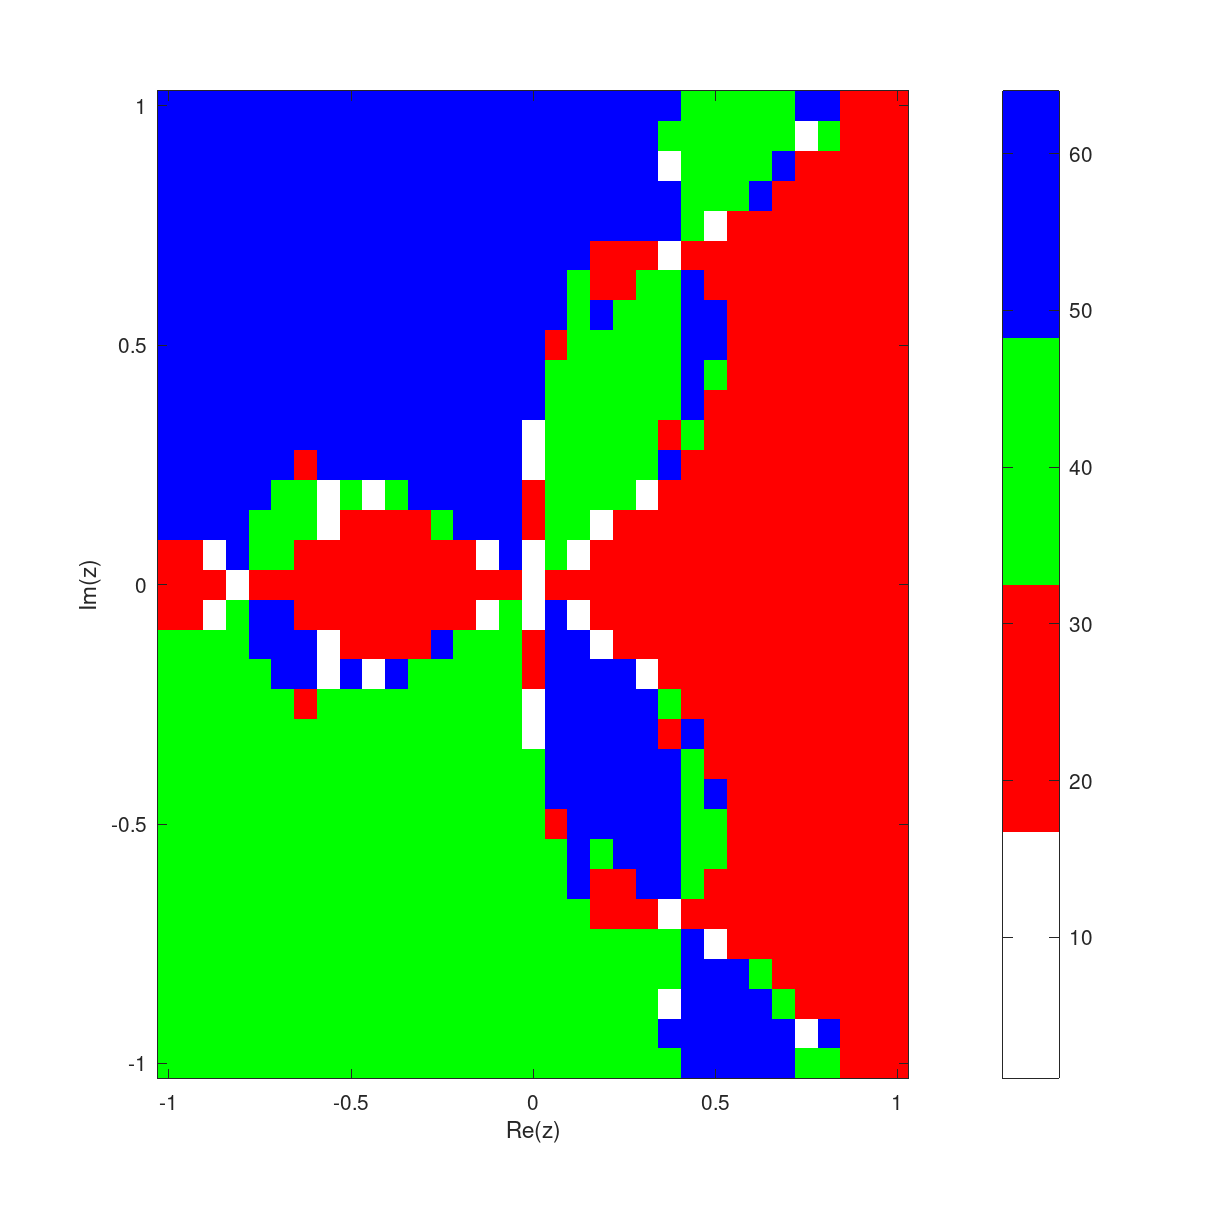
\includegraphics[width=152mm, height=120mm]{images/L2n32maxit16e10-10color.png}
    \caption{$L=2$, $n=32$, maxit $=16$, $\epsilon=10^{-10}$ con colores}
\end{figure}

\begin{figure}[H]
    \centering
    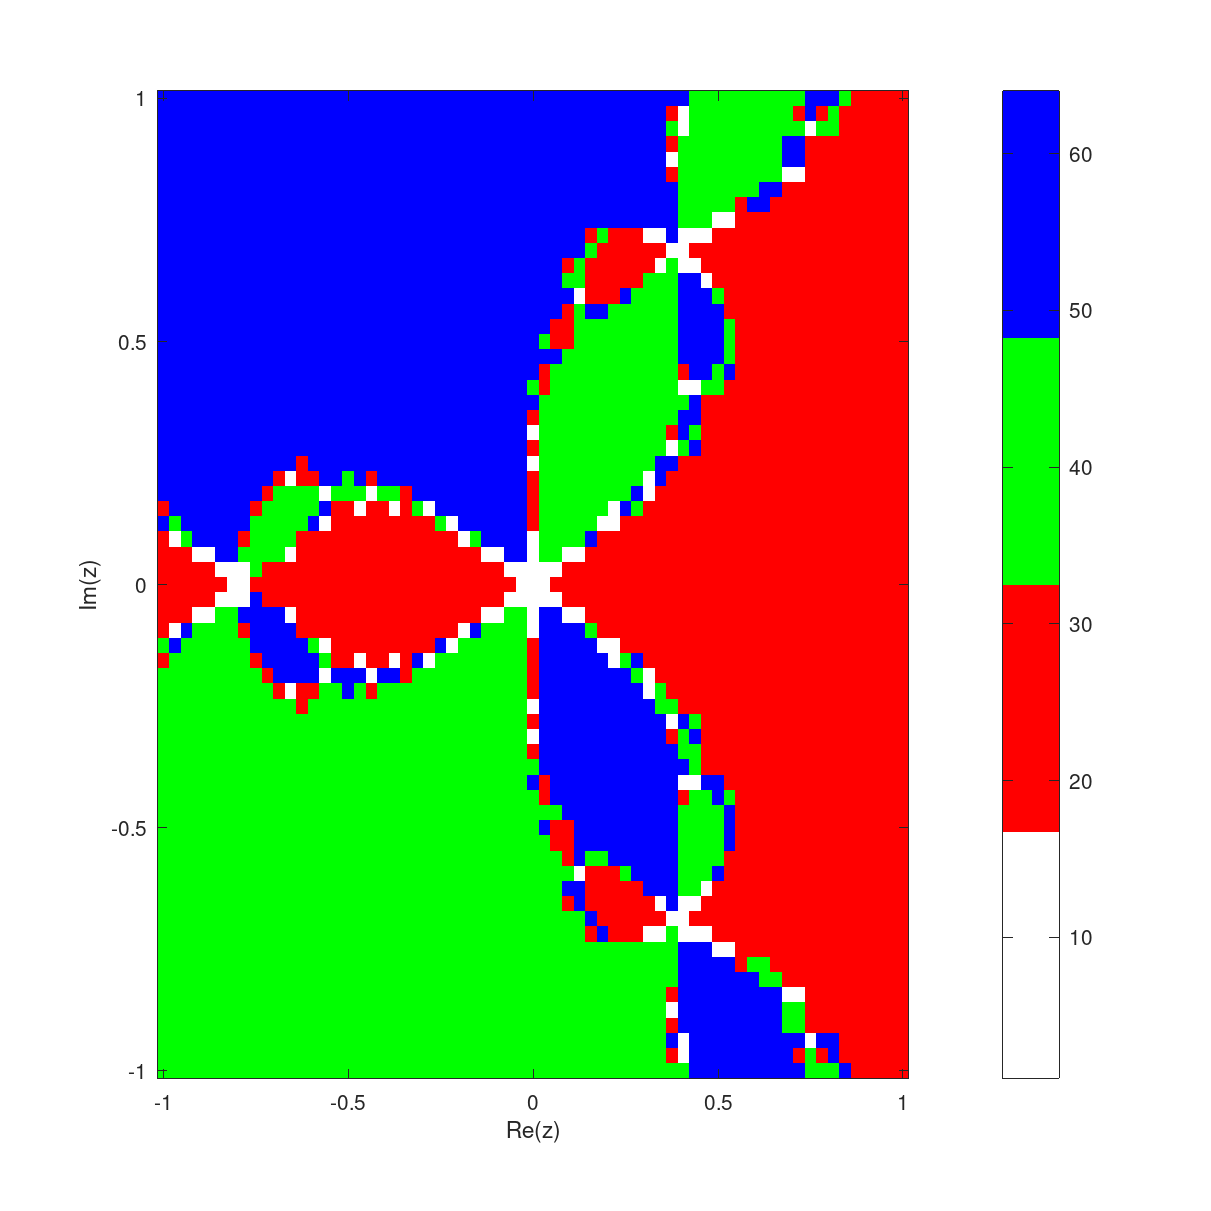
\includegraphics[width=152mm, height=120mm]{images/L2n64maxit16e10-10color.png}
    \caption{$L=2$, $n=64$, maxit $=16$, $\epsilon=10^{-10}$ con colores}
\end{figure}

\begin{figure}[H]
    \centering
    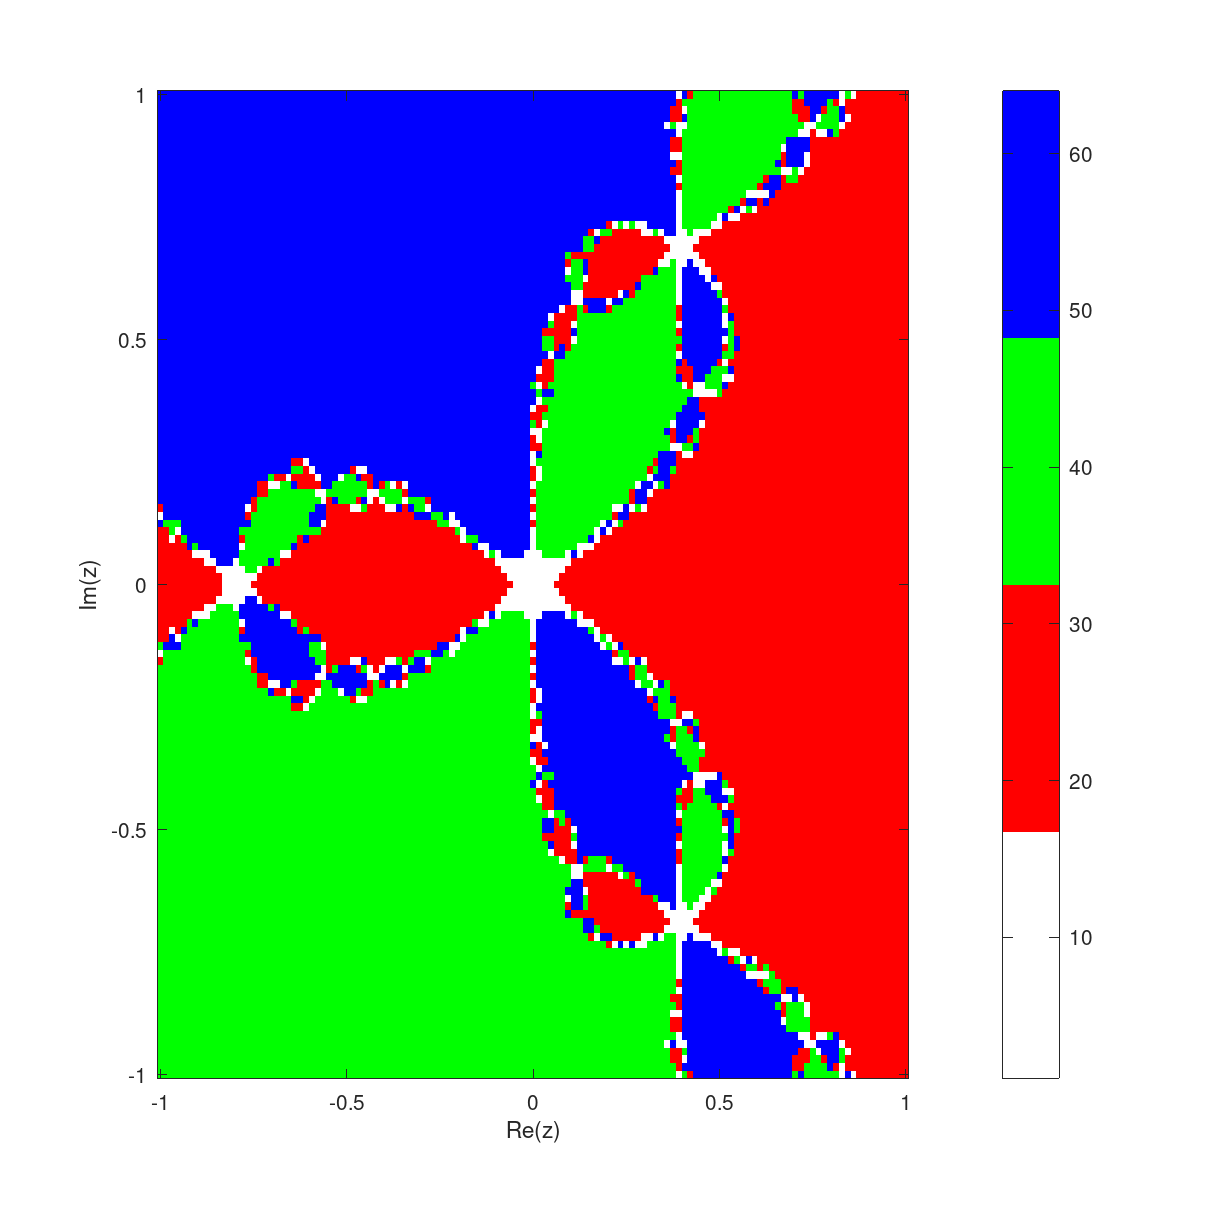
\includegraphics[width=152mm, height=120mm]{images/L2n128maxit16e10-10color.png}
    \caption{$L=2$, $n=128$, maxit $=16$, $\epsilon=10^{-10}$ con colores}
\end{figure}

\begin{figure}[H]
    \centering
    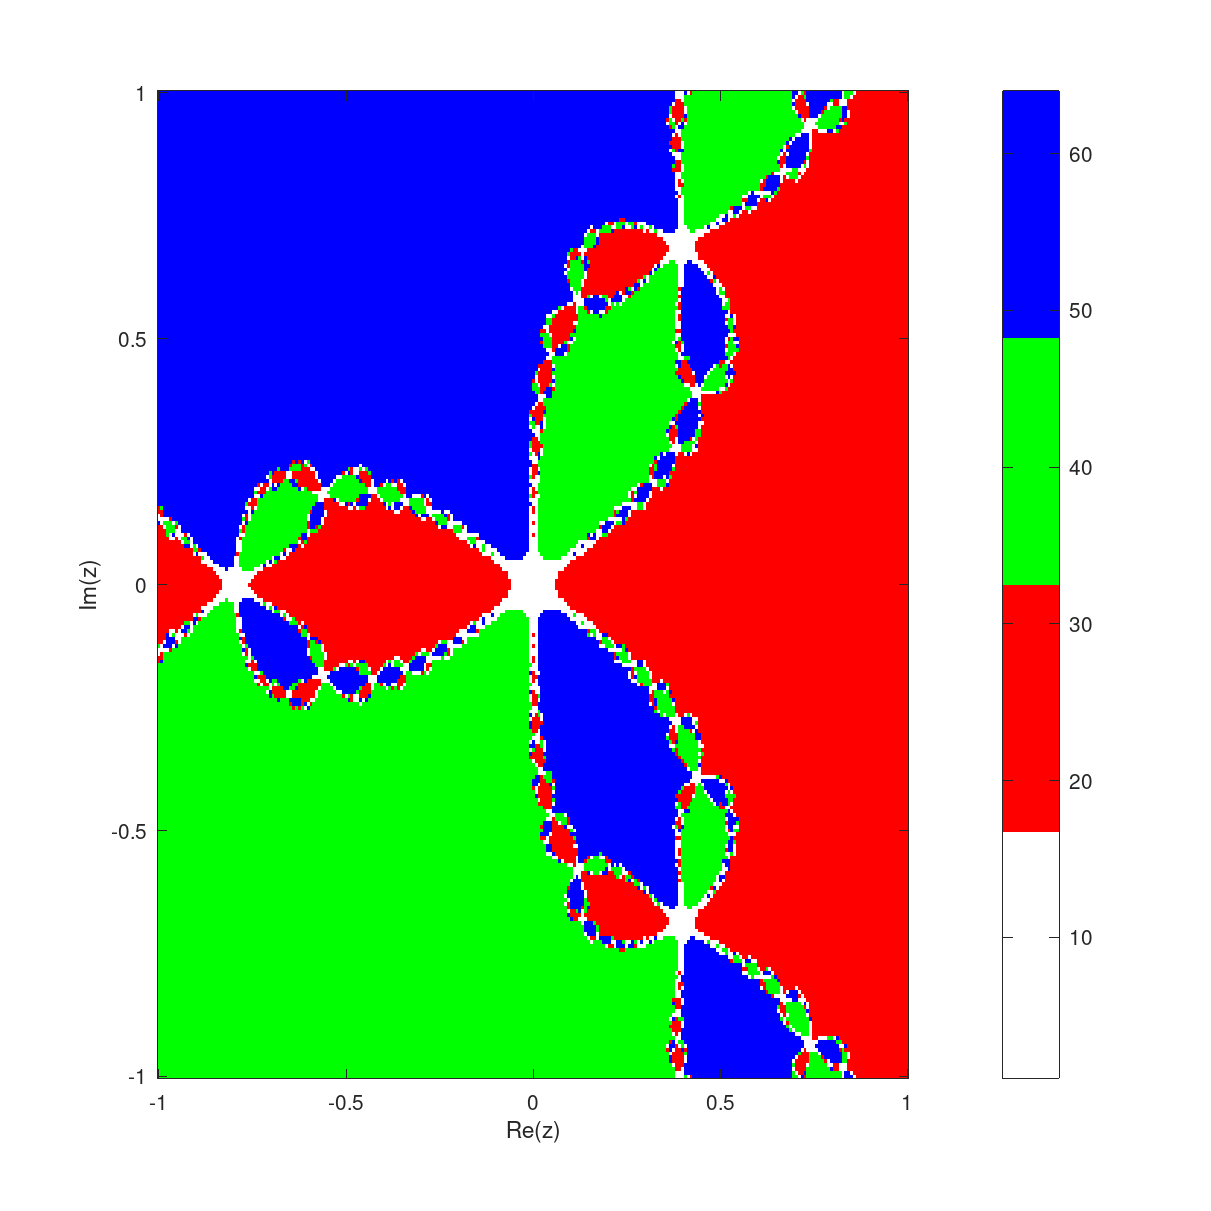
\includegraphics[width=152mm, height=120mm]{images/L2n256maxit16e10-10color.png}
    \caption{$L=2$, $n=256$, maxit $=16$, $\epsilon=10^{-10}$ con colores}
\end{figure}

\begin{figure}[H]
    \centering
    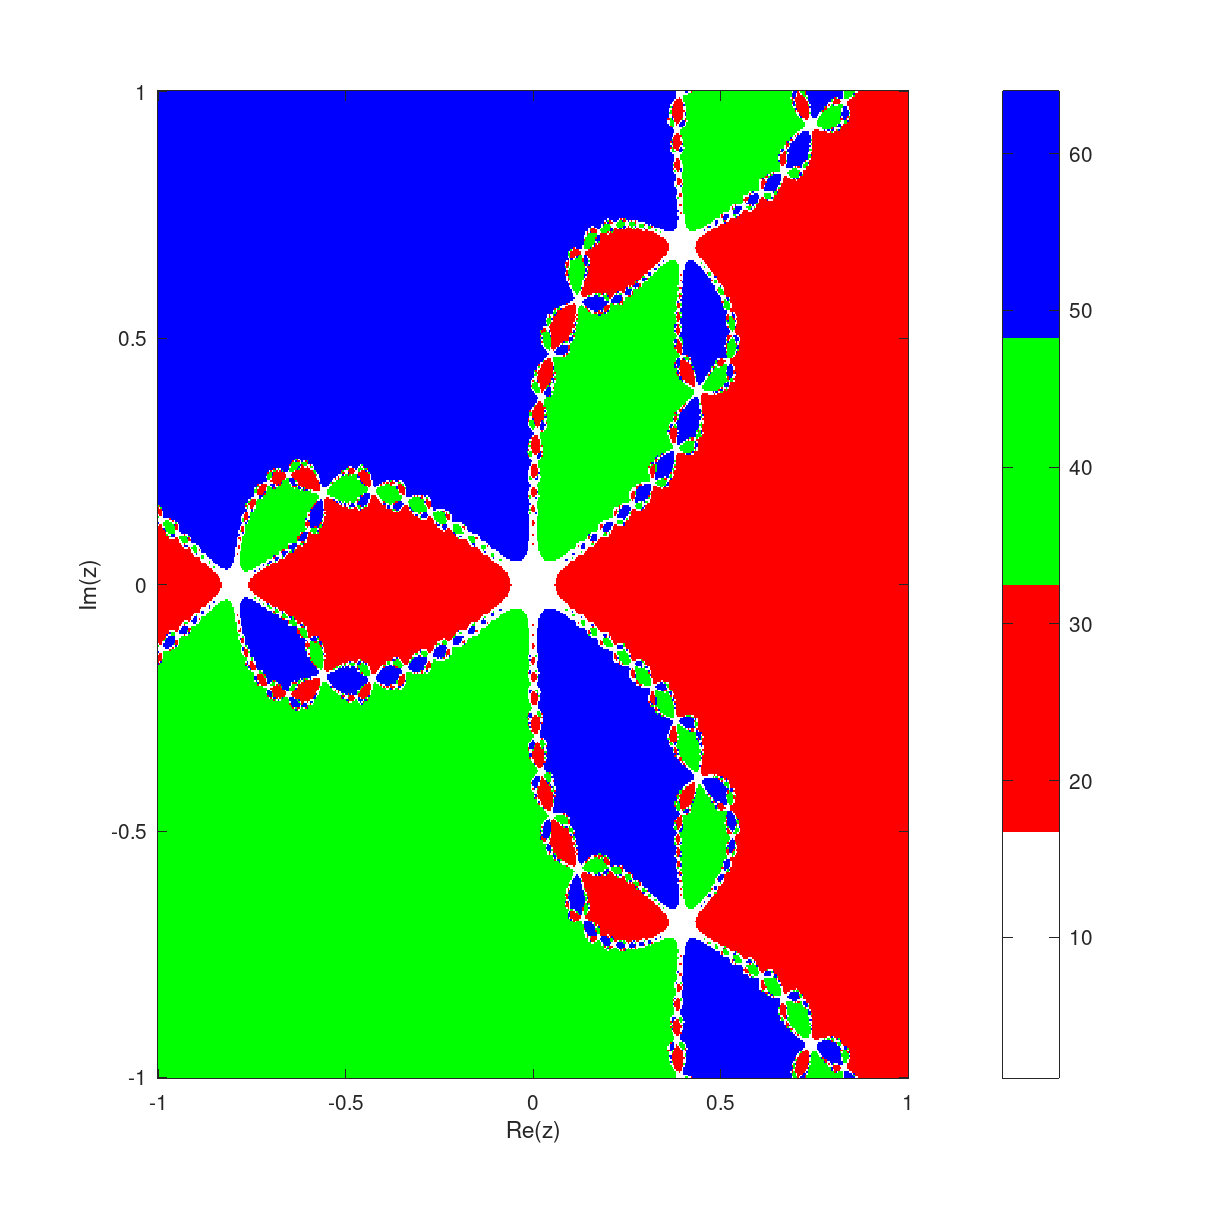
\includegraphics[width=152mm, height=120mm]{images/L2n512maxit16e10-10color.png}
    \caption{$L=2$, $n=512$, maxit $=16$, $\epsilon=10^{-10}$ con colores}
\end{figure}

\newpage

\textbf{c.} Tome ahora $L=2$, $n=256$, $\epsilon=10^{-10}$ y tome maxit = 32. Como el caso anterior, pinte de un color de acuerdo a la raíz a la que llegue pero ahora, en el caso en que llegue a una raíz pinte tonalidades del color correspondiente de acuerdo al numero de iteraciones del método de Newton.

\begin{figure}[H]
    \centering
    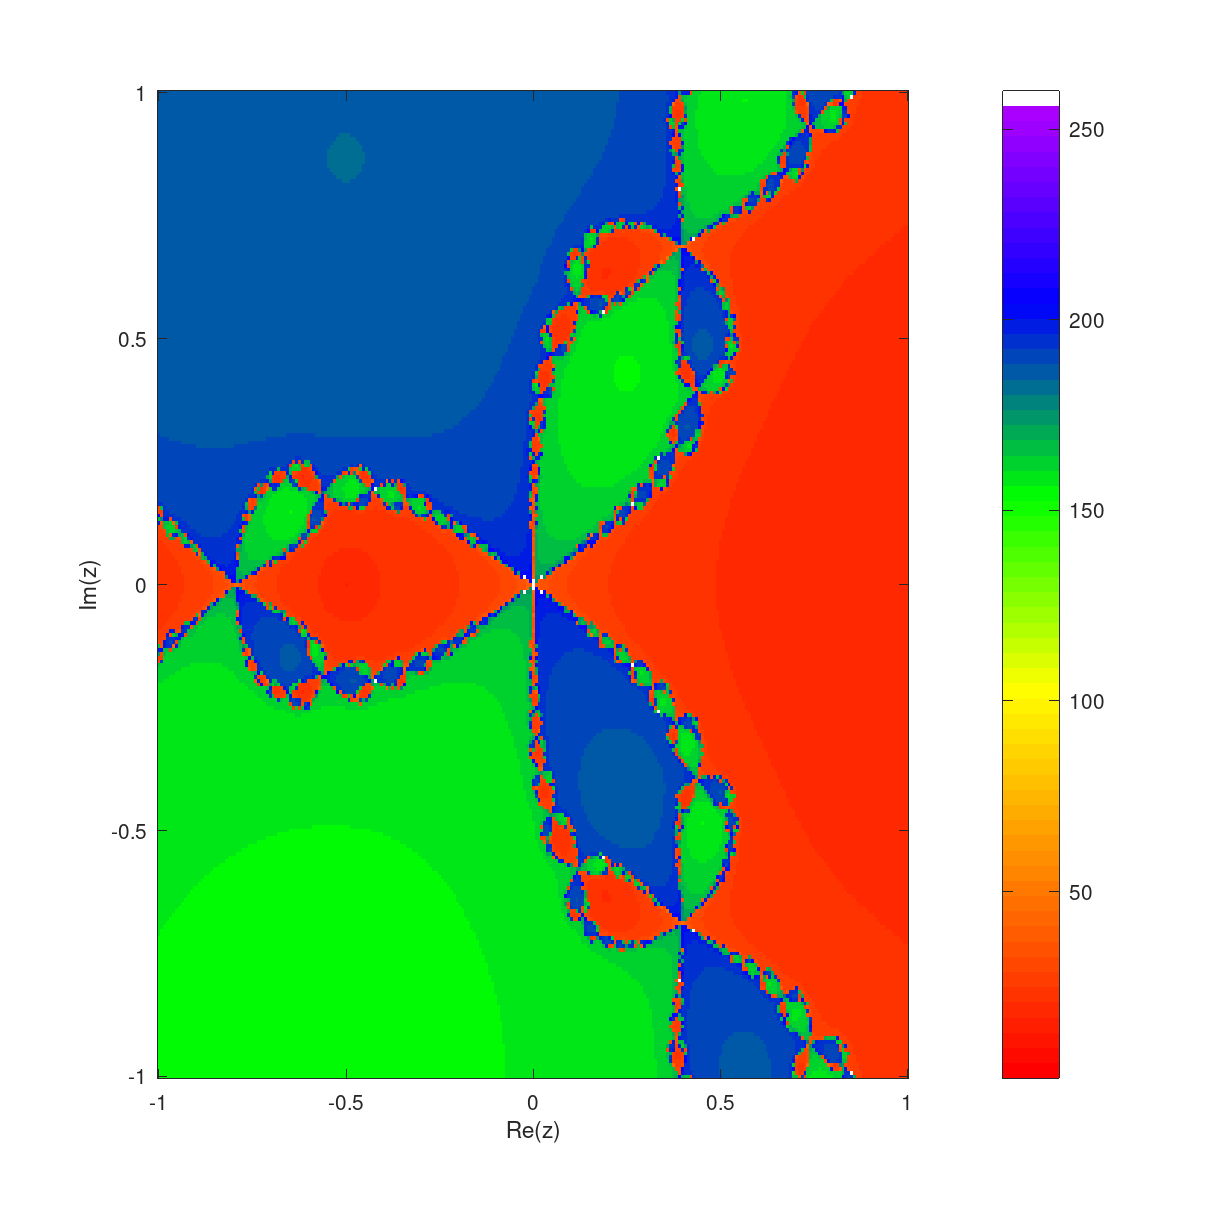
\includegraphics[width=152mm, height=120mm]{images/L2n256maxit32e10-10colordegradado.png}
    \caption{$L=2$, $n=256$, maxit $=32$, $\epsilon=10^{-10}$ con colores según iteraciones}
\end{figure}

\textbf{d.} Repita el inciso anterior pero ahora tome $n=512$ y $n=1024$ con maxit = 32 y 64.

\begin{figure}[H]
    \centering
    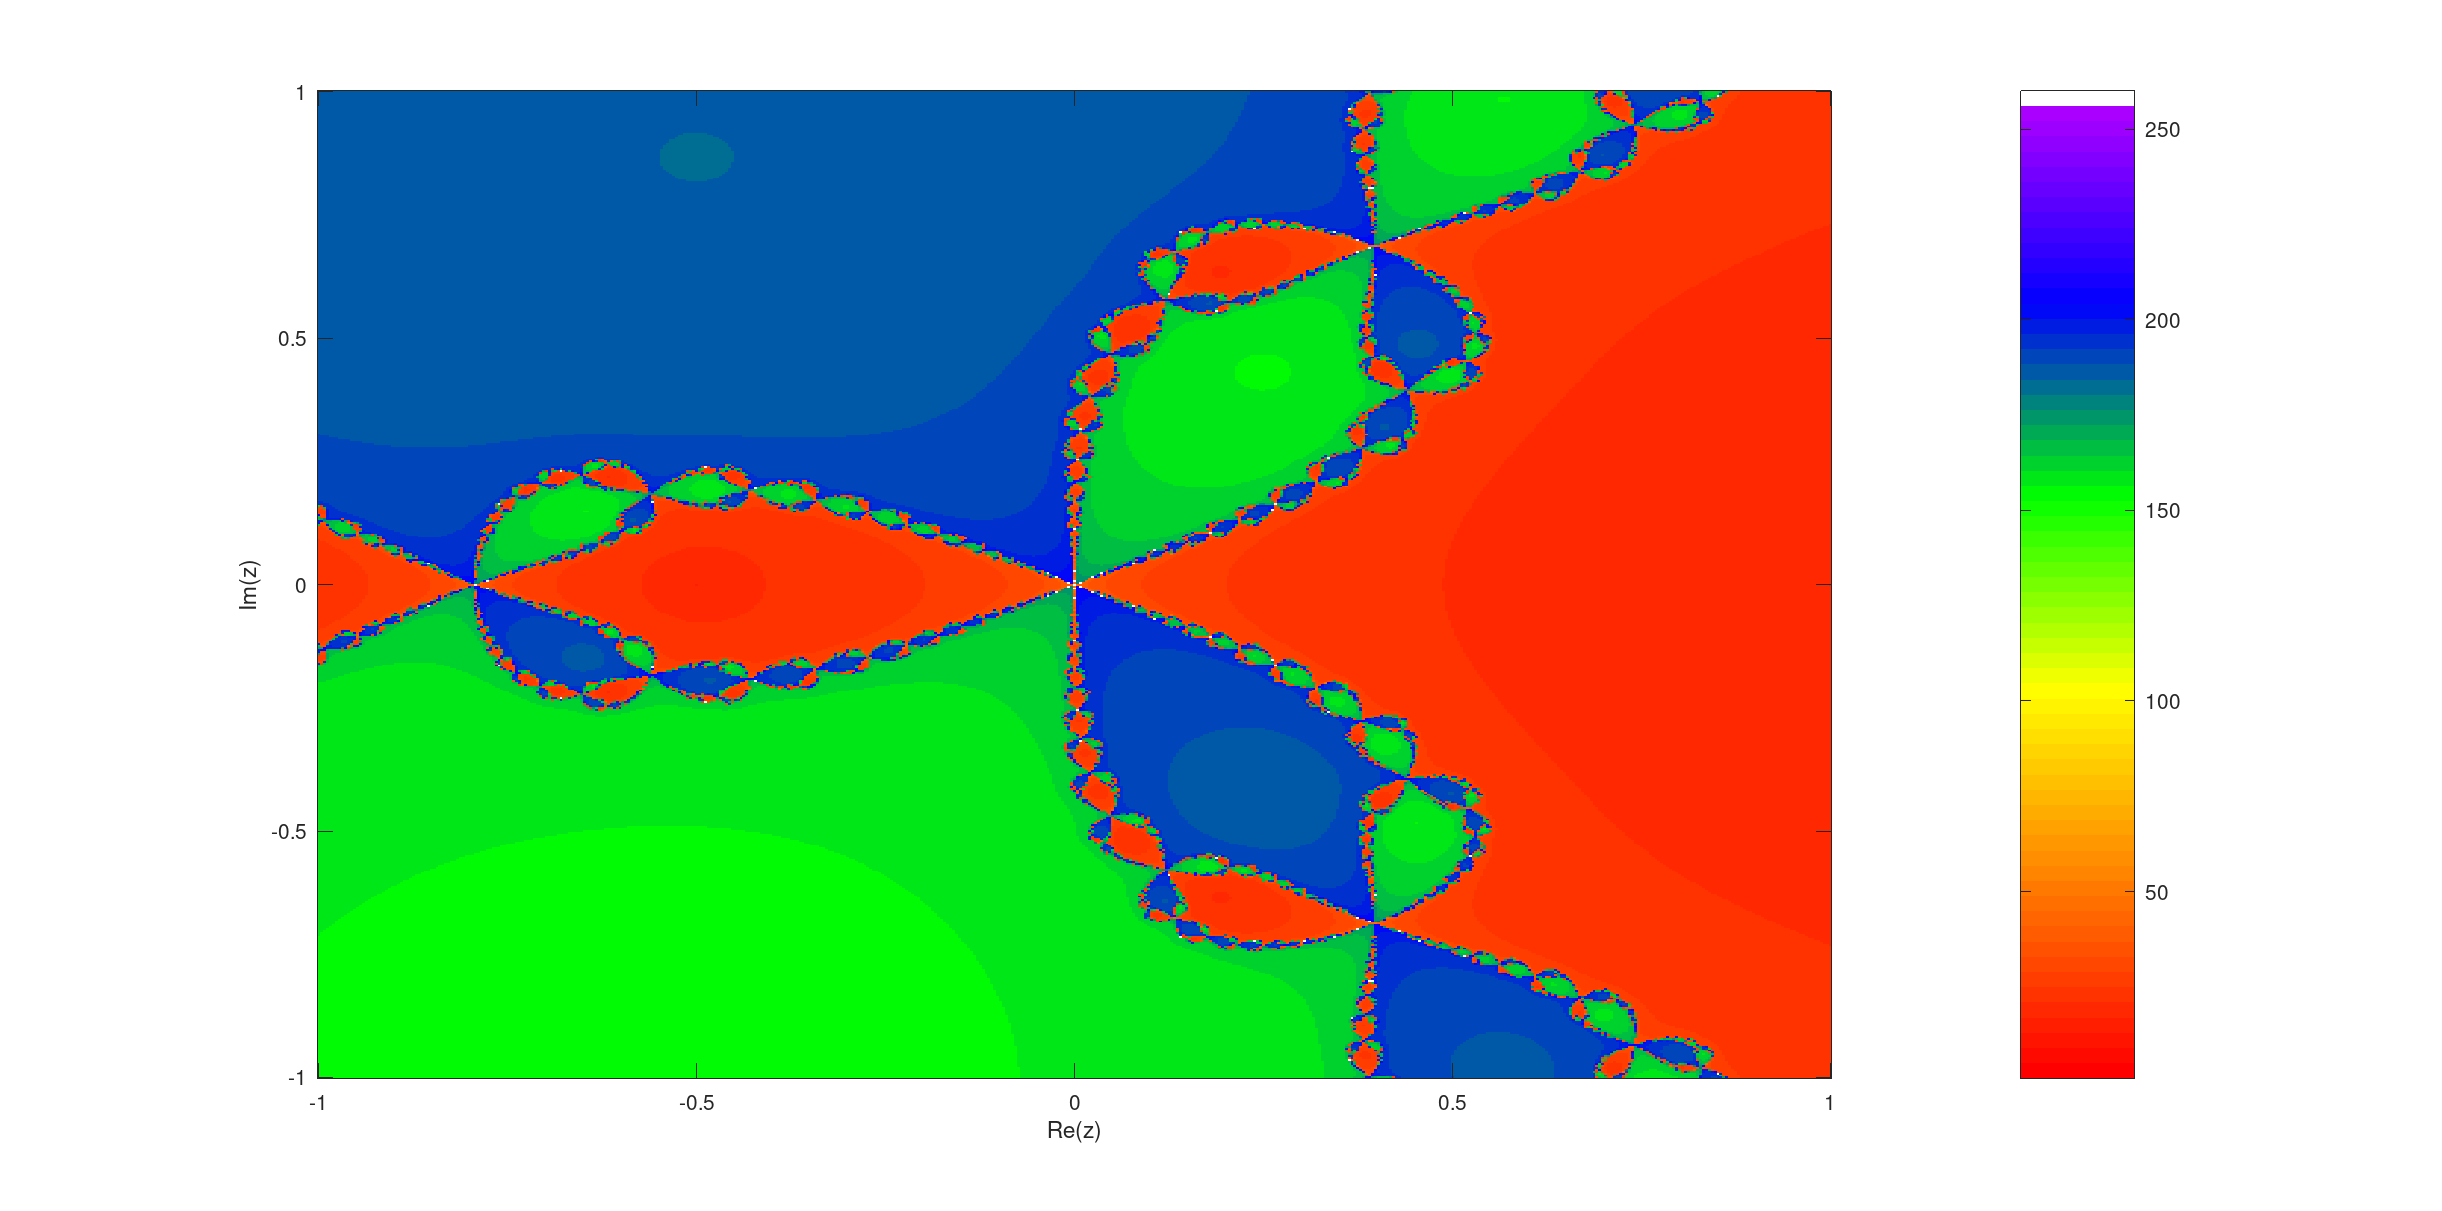
\includegraphics[width=152mm, height=120mm]{images/L2n512maxit32e10-10colordegradado.png}
    \caption{$L=2$, $n=512$, maxit $=32$, $\epsilon=10^{-10}$ con colores según iteraciones}
\end{figure}

\begin{figure}[H]
    \centering
    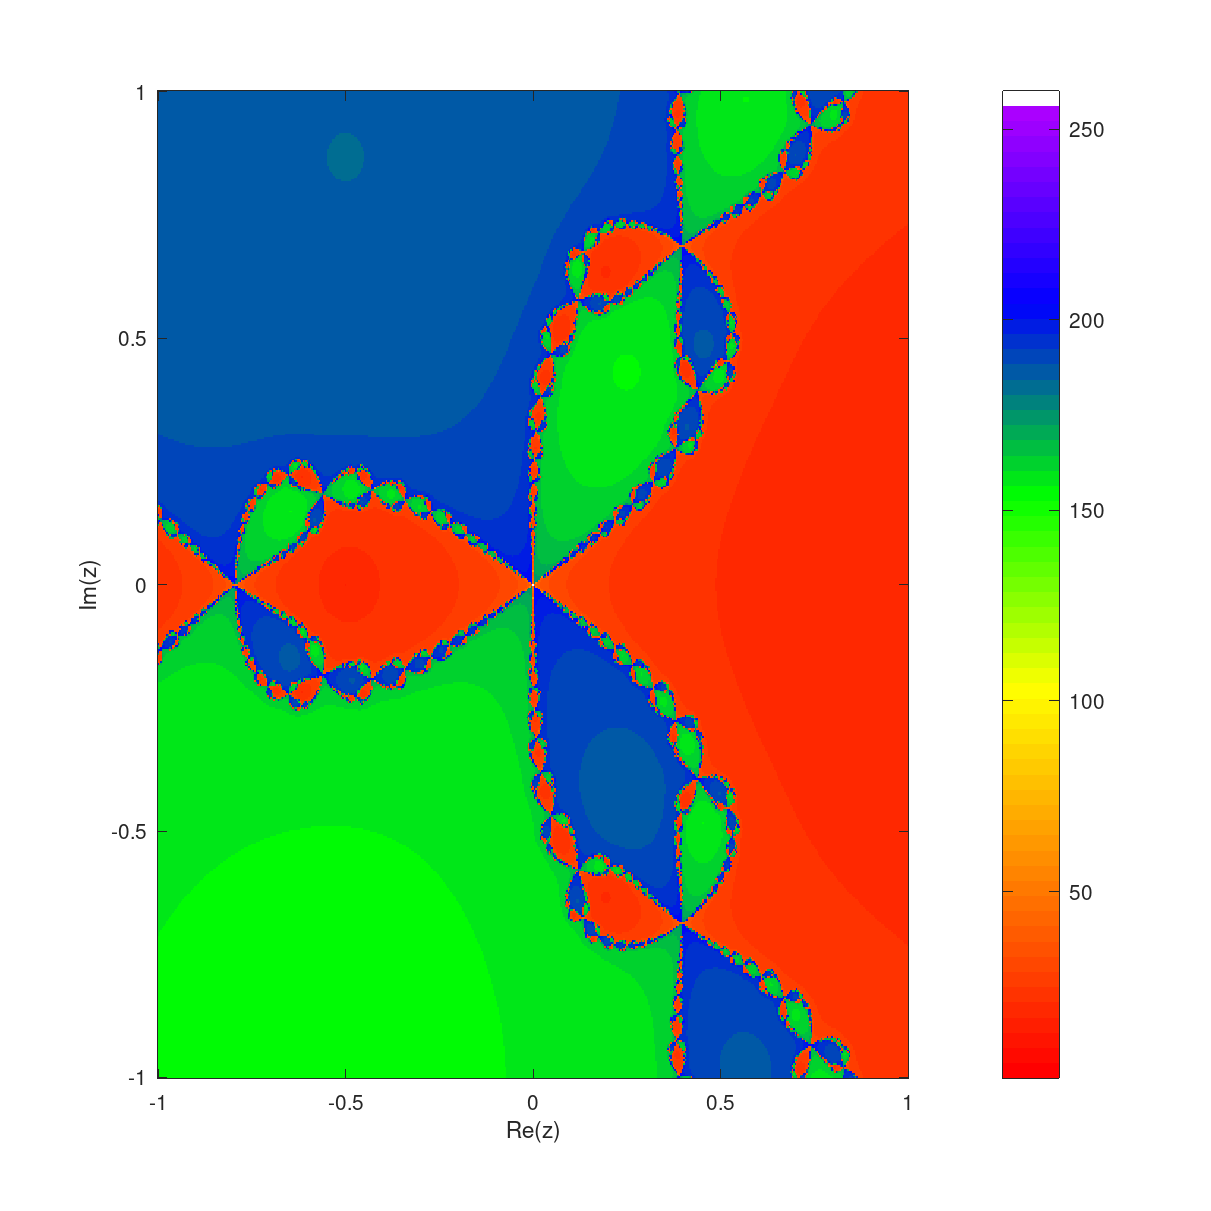
\includegraphics[width=152mm, height=120mm]{images/L2n512maxit64e10-10colordegradado.png}
    \caption{$L=2$, $n=512$, maxit $=64$, $\epsilon=10^{-10}$ con colores según iteraciones}
\end{figure}

\begin{figure}[H]
    \centering
    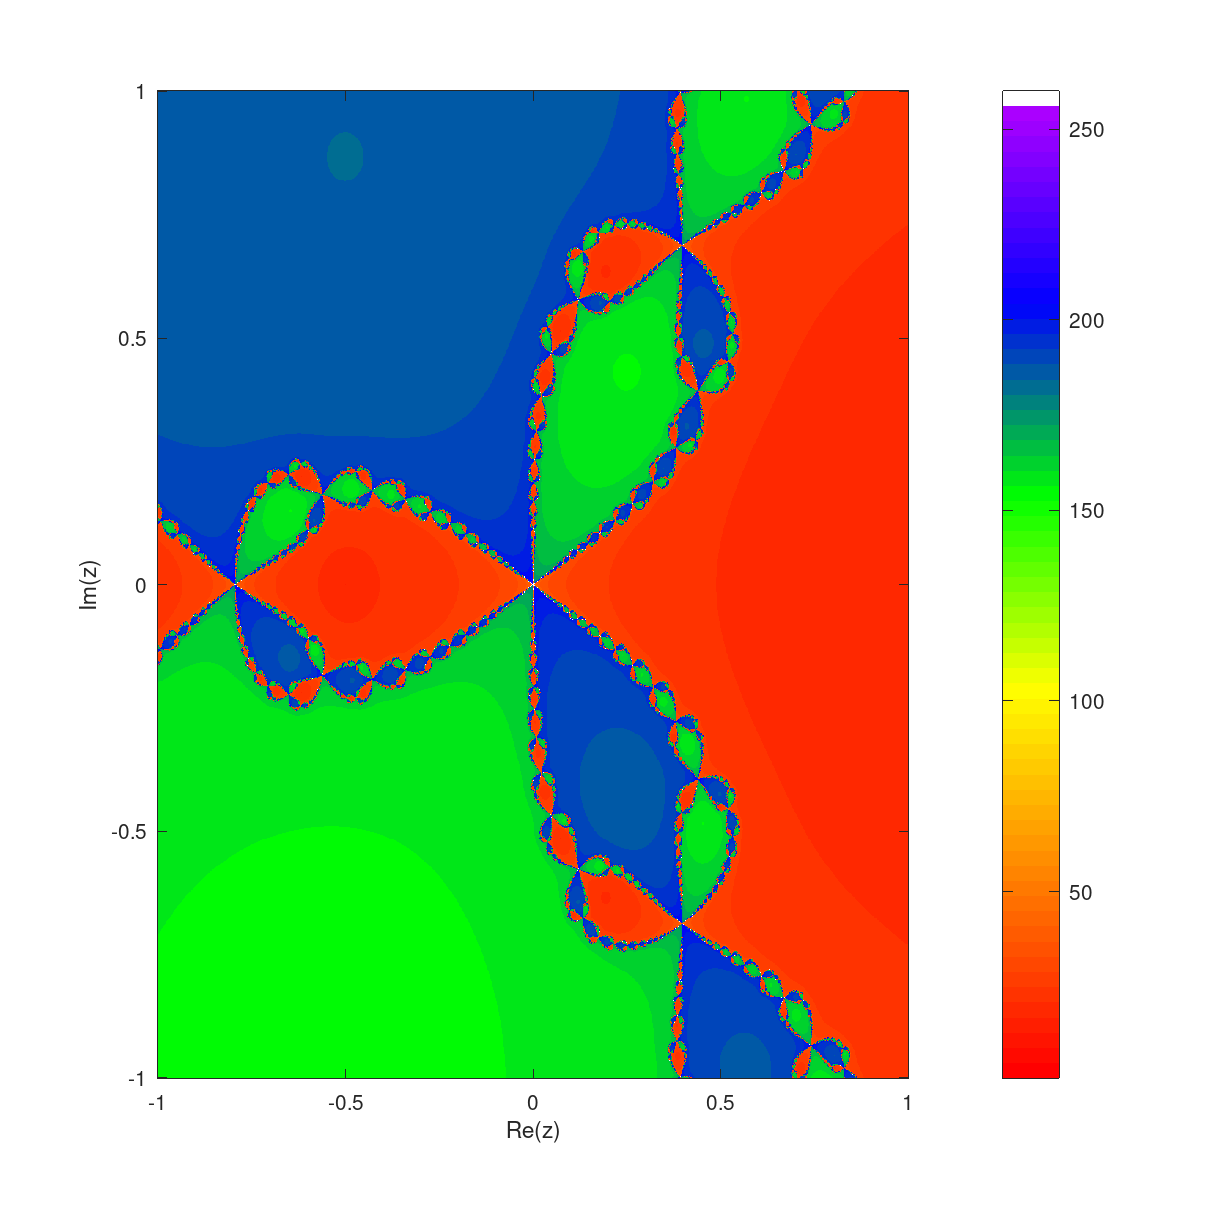
\includegraphics[width=152mm, height=120mm]{images/L2n1024maxit32e10-10colordegradado.png}
    \caption{$L=2$, $n=1024$, maxit $=32$, $\epsilon=10^{-10}$ con colores según iteraciones}
\end{figure}

\begin{figure}[H]
    \centering
    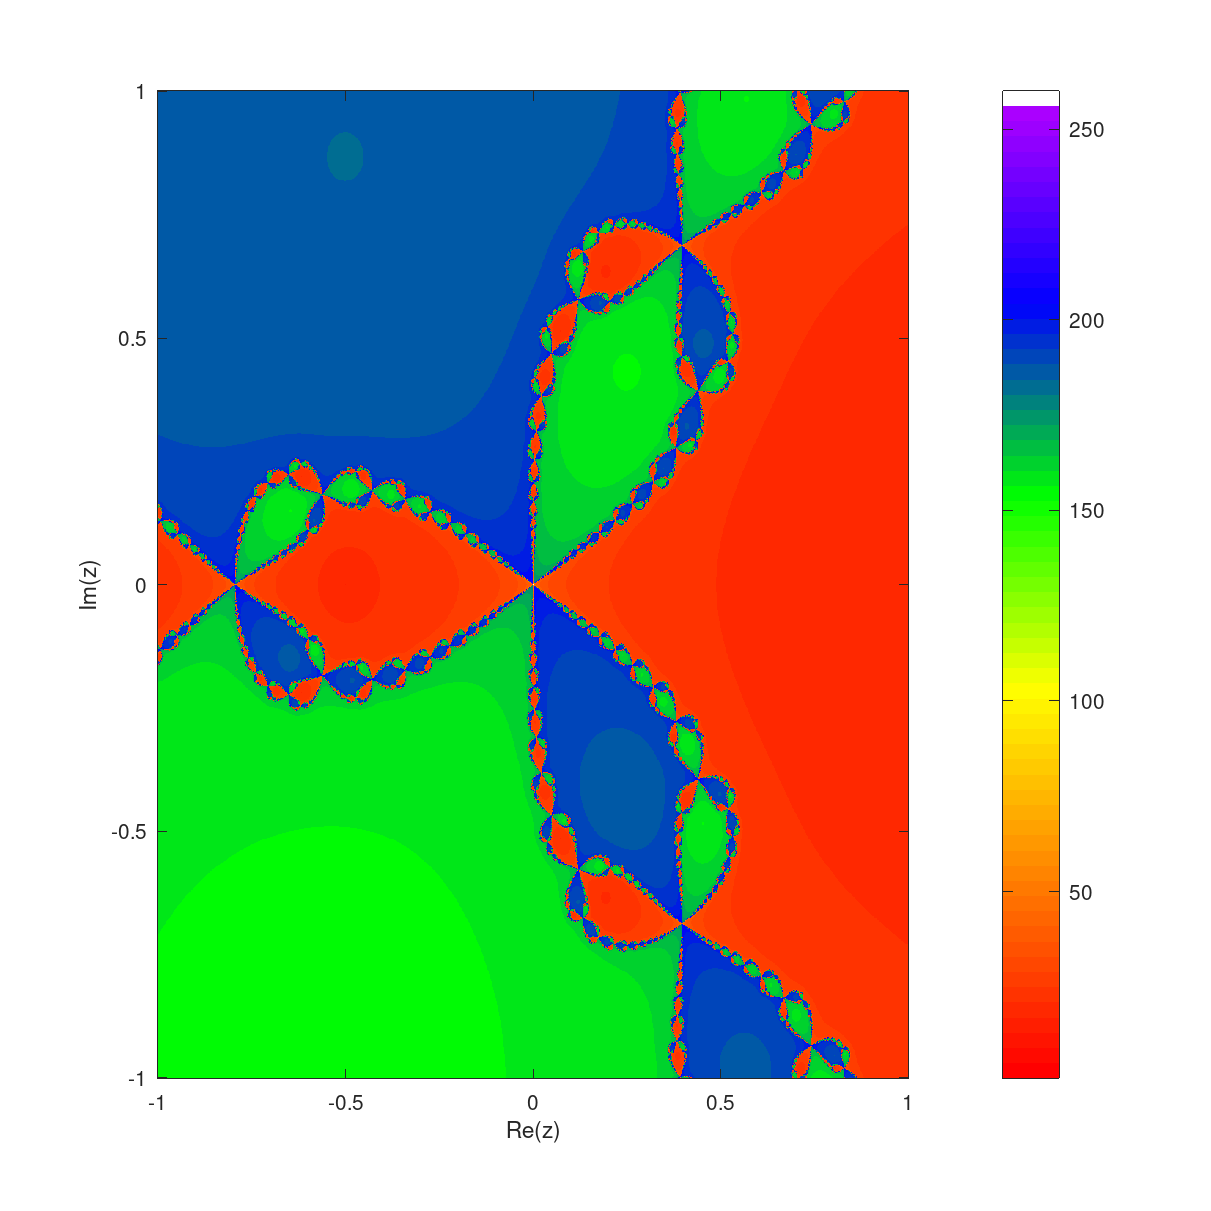
\includegraphics[width=152mm, height=120mm]{images/L2n1024maxit64e10-10colordegradado.png}
    \caption{$L=2$, $n=1024$, maxit $=64$, $\epsilon=10^{-10}$ con colores según iteraciones}
\end{figure}



\end{document}
